%% (Master) Thesis template
% Template version used: v1.4
%
% Largely adapted from Adrian Nievergelt's template for the ADPS
% (lecture notes) project.



%% We use the memoir class because it offers a many easy to use features.
\documentclass[11pt,a4paper,table,hidelinks]{memoir}  % Remove "hidelinks" for red boxes around hyperlinks

%% Packages
%% ========

%% LaTeX Font encoding -- DO NOT CHANGE
\usepackage[OT1]{fontenc}

%% Babel provides support for languages.  'english' uses British
%% English hyphenation and text snippets like "Figure" and
%% "Theorem". Use the option 'ngerman' if your document is in German.
%% Use 'american' for American English.  Note that if you change this,
%% the next LaTeX run may show spurious errors.  Simply run it again.
%% If they persist, remove the .aux file and try again.
\usepackage[english]{babel}

%% Input encoding 'utf8'. In some cases you might need 'utf8x' for
%% extra symbols. Not all editors, especially on Windows, are UTF-8
%% capable, so you may want to use 'latin1' instead.
\usepackage[utf8]{inputenc}

%% This changes default fonts for both text and math mode to use Herman Zapfs
%% excellent Palatino font.  Do not change this.
%\usepackage[sc]{mathpazo}

%% The AMS-LaTeX extensions for mathematical typesetting.  Do not
%% remove.
\usepackage{amsmath,amssymb,amsfonts,mathrsfs}

%% NTheorem is a reimplementation of the AMS Theorem package. This
%% will allow us to typeset theorems like examples, proofs and
%% similar.  Do not remove.
%% NOTE: Must be loaded AFTER amsmath, or the \qed placement will
%% break
\usepackage[amsmath,thmmarks]{ntheorem}

%% LaTeX' own graphics handling
\usepackage{graphicx}

%% We unfortunately need this for the Rules chapter.  Remove it
%% afterwards; or at least NEVER use its underlining features.
\usepackage{soul}

%% This allows you to add .pdf files. It is used to add the
%% declaration of originality.
\usepackage{pdfpages}

\newenvironment{conditions}
  {\par\vspace{\abovedisplayskip}\noindent\begin{tabular}{>{$}l<{$} @{${}={}$} l}}
  {\end{tabular}\par\vspace{\belowdisplayskip}}

%% Some more packages that you may want to use.  Have a look at the
%% file, and consult the package docs for each.
%% See the TeXed file for more explanations

%% [OPT] Multi-rowed cells in tabulars
%\usepackage{multirow}

%% [REC] Intelligent cross reference package. This allows for nice
%% combined references that include the reference and a hint to where
%% to look for it.
\usepackage{varioref}

%% [OPT] Easily changeable quotes with \enquote{Text}
%\usepackage[german=swiss]{csquotes}

%% [REC] Format dates and time depending on locale
\let\ordinal\relax %% prevent warning
\usepackage{datetime}

%% [OPT] Provides a \cancel{} command to stroke through mathematics.
%\usepackage{cancel}

%% [NEED] This allows for additional typesetting tools in mathmode.
%% See its excellent documentation.
\usepackage{mathtools}

%% [NEED] Conditional commands
\usepackage{ifthen}

%% [OPT] Manual large braces or other delimiters.
%\usepackage{bigdelim, bigstrut}

%% [REC] Alternate vector arrows. Use the command \vv{} to get scaled
%% vector arrows.
\usepackage[h]{esvect}

%% [NEED] Some extensions to tabulars and array environments.
\usepackage{array}

%% [OPT] Postscript support via pstricks graphics package. Very
%% diverse applications.
%\usepackage{pstricks,pst-all}

%% [?] This seems to allow us to define some additional counters.
%\usepackage{etex}

%% [ADV] XY-Pic to typeset some matrix-style graphics
%\usepackage[all]{xy}

%% [OPT] This is needed to generate an index at the end of the
%% document.
%\usepackage{makeidx}

%% [OPT] Fancy package for source code listings.  The template text
%% needs it for some LaTeX snippets; remove/adapt the \lstset when you
%% remove the template content.
\usepackage{listings}
% \lstset{language=TeX,basicstyle={\normalfont\ttfamily}}

%% [REC] Fancy character protrusion.  Must be loaded after all fonts.
%\usepackage[activate]{pdfcprot}

%% [REC] Nicer tables.  Read the excellent documentation.
\usepackage{booktabs}

%% [OPT] Package for adding TODOs.
\usepackage{todonotes}

%% [OPT] Package to define and use acronyms
\usepackage[nolist,nohyperlinks,smaller]{acronym}
 

%% Our layout configuration.  DO NOT CHANGE.
%% Memoir layout setup

%% NOTE: You are strongly advised not to change any of them unless you
%% know what you are doing.  These settings strongly interact in the
%% final look of the document.

% Dependencies
%\usepackage{ETHlogo}

% use helvetica as default font:
\usepackage[scaled]{helvet}
%\renewcommand\familydefault{\sfdefault} 

% Turn extra space before chapter headings off.
\setlength{\beforechapskip}{0pt}

\nonzeroparskip
\parindent=0pt
\defaultlists

% Chapter style redefinition
\makeatletter

\makepagestyle{headerWPageNr}% Create headerWPageNr style
\if@twoside
  \copypagestyle{headerWPageNr}{Ruled}
  \copypagestyle{chapter}{Ruled}
\else
  \copypagestyle{headerWPageNr}{ruled}
  \copypagestyle{chapter}{ruled}
\fi
% chapter pages have no header and center page number in footer:
\makeoddhead{chapter}{}{}{}
\makeevenhead{chapter}{}{}{}
\makeoddfoot{chapter}{}{\thepage}{}
\makeevenfoot{chapter}{}{\thepage}{}
\makeheadrule{chapter}{\textwidth}{0pt}

% all other pages have page number and chapter or section name in header without footer:
\makeoddhead{headerWPageNr}{\rightmark}{}{\thepage}
\makeevenhead{headerWPageNr}{\thepage}{}{\leftmark}
\makeoddfoot{headerWPageNr}{}{}{}
\makeevenfoot{headerWPageNr}{}{}{}
\pagestyle{headerWPageNr}% Set page style to headerWPageNr


\makechapterstyle{bianchimod}{%
  \copypagestyle{abstract}{empty}
  \chapterstyle{default}
  \renewcommand*{\chapnamefont}{\normalfont\Large\sffamily}
  \renewcommand*{\chapnumfont}{\normalfont\Large\sffamily}
  \renewcommand*{\printchaptername}{%
    \chapnamefont\centering\@chapapp}
  \renewcommand*{\printchapternum}{\chapnumfont {\thechapter}}
  \renewcommand*{\chaptitlefont}{\normalfont\huge\sffamily}
  \renewcommand*{\printchaptertitle}[1]{%
    \hrule\vskip\onelineskip \centering \chaptitlefont\textbf{\vphantom{gyM}##1}\par}
  \renewcommand*{\afterchaptertitle}{\vskip\onelineskip \hrule\vskip
    \afterchapskip}
  \renewcommand*{\printchapternonum}{%
    \vphantom{\chapnumfont {9}}\afterchapternum}}
  
\makechapterstyle{bianchimod2}{%
  \renewenvironment{abstract}{\chapter*{\abstractname}}{}
  \chapterstyle{default}
  \definecolor{ChapGrey}{rgb}{0.6,0.6,0.6}
  \newcommand{\LargeFont}{% Needs a ’stretchable’ font
  	\usefont{\encodingdefault}{\sfdefault}{b}{n}%
    \fontsize{100}{0}\selectfont\color{ChapGrey}}
  \renewcommand*{\chapnumfont}{\LargeFont}
  \renewcommand*{\printchaptername}{\raggedleft}
  \renewcommand*{\printchapternum}{\chapnumfont {\thechapter}}
  \renewcommand*{\chaptitlefont}{\normalfont\Huge\sffamily\color{black}}
  \renewcommand*{\printchaptertitle}[1]{%
    \raggedleft \chaptitlefont\textbf{\vphantom{gyM}##1}\par}}

% Use the newly defined style
\chapterstyle{bianchimod2}

\setsecheadstyle{\Large\bfseries\sffamily}
\setsubsecheadstyle{\large\bfseries\sffamily}
\setsubsubsecheadstyle{\bfseries\sffamily}
\setparaheadstyle{\normalsize\bfseries\sffamily}
\setsubparaheadstyle{\normalsize\itshape\sffamily}
\setsubparaindent{0pt}

% Set captions to a more separated style for clearness
\captionnamefont{\sffamily\bfseries\footnotesize}
\captiontitlefont{\sffamily\footnotesize}
\setlength{\intextsep}{16pt}
\setlength{\belowcaptionskip}{1pt}

% Set section and TOC numbering depth to subsection
\setsecnumdepth{subsection}
\settocdepth{subsection}

% definitions for titlepage
\def\@advisor{}
\newcommand{\advisor}[1]{\def\@advisor{#1}}
\def\@supervisor{}
\newcommand{\supervisor}[1]{\def\@supervisor{#1}}
\def\@group{}
\newcommand{\group}[1]{\def\@group{#1}}
\def\@institute{}
\newcommand{\institute}[1]{\def\@institute{#1}}
\def\@department{}
\newcommand{\department}[1]{\def\@department{#1}}
\def\@school{}
\newcommand{\school}[1]{\def\@school{#1}}
\def\@thesistype{}
\newcommand{\thesistype}[1]{\def\@thesistype{#1}}
\def\@email{}
\newcommand{\email}[1]{\def\@email{#1}}

%% Title page adjustments
% the following definition (either 0 or 1) controls the title page's layout:
\def\centeredtitlepage{0}
\if\centeredtitlepage1
	% default title page from cadmo template
	\newcommand{\maketitlepage}{
		\begin{titlingpage}
  			\calccentering{\unitlength}
  			\begin{adjustwidth*}{\unitlength-24pt}{-\unitlength-24pt}
    		\maketitle
  			\end{adjustwidth*}
		\end{titlingpage}
	}
	\pretitle{\vspace{0pt plus 0.7fill}\begin{center}\HUGE\sffamily\bfseries}
	\posttitle{\end{center}\par}
	\preauthor{\par\begin{center}\let\and\\\Large\sffamily}
	\postauthor{\end{center}}
	\predate{\par\begin{center}\Large\sffamily}
	\postdate{\end{center}}

	\renewcommand{\maketitlehooka}{\noindent\ETHlogo[2in]}

	\renewcommand{\maketitlehookb}{\vspace{1in}%
  		\par\begin{center}\Large\sffamily\@thesistype\end{center}}

	\renewcommand{\maketitlehookd}{%
  		\vfill\par
  			\begin{flushright}
    			\sffamily
    			Advisors: \@supervisor, \@advisor\par
    			\@department, \@school
  			\end{flushright}
	}

\else
	% alternative title page (right-aligned)
	\newcommand{\maketitlepage}{
		\begin{titlingpage}
			\titlestyleright
		\end{titlingpage}
	}
	\newcommand*\titlestyleright{
		\thispagestyle{empty}
		\begin{minipage}[c]{0.35\linewidth}
			\vspace{0pt}
			\hfuzz=5.0pt
			
\includegraphics[width=0.9\linewidth]{images/ost_logo_de_rgb-eps-converted-to}
		\end{minipage}
		%
		\begin{minipage}[c]{0.4\linewidth}
			\vspace{0pt}
			\-\
		\end{minipage}
		%
		\begin{minipage}[c]{0.25\linewidth}
			\vspace{0pt}
			\hfuzz=5.0pt
			    \hspace*{-1cm} 
			        
\includegraphics[width=1.3\linewidth]{images/onway_logo}
		\end{minipage}
		\vspace{2cm}
		\sffamily
		\vspace*{\stretch{6}}
		\begin{flushright}
		{\Huge\sffamily\bfseries\@title\par}
		\par\noindent\rule[-1ex]{\linewidth}{2pt}\par
		\vspace{0.5cm}
		\emph{\huge\sffamily\@thesistype}
		\vspace{2cm}\par
		{\LARGE\sffamily\bfseries Florian Baumgartner}\par
		{\sffamily\ \href{mailto:florian.baumgartner@ost.ch}{florian.baumgartner@ost.ch}}\par
		\vspace{0.5cm}
		{\LARGE\sffamily\bfseries Luca Jost}\par
		{\sffamily\ \href{mailto:luca.jost@ost.ch}{luca.jost@ost.ch}}\par
		\vspace{1cm}
    	{\large\textbf{Advisor}\par
    		\@advisor\par}
    	\vspace{0.5cm}
    	{\large\textbf{Examiner}\par
    		\@supervisor\par}
    	\vspace{1cm}
    	{\@institute\par
        	\@school\par}
    	\vspace{1cm}
    	{\normalsize\@date\par}
		\end{flushright}
		\vspace{\stretch{1}}
		\noindent
		\pagebreak 
    	\sffamily
    	\thispagestyle{empty} 
	}
\fi

%Change margins
\setlrmarginsandblock{3.5cm}{3cm}{*}
\setulmarginsandblock{3cm}{*}{1}
\checkandfixthelayout

\setlength{\droptitle}{-48pt}

\makeatother

% This defines how theorems should look. Best leave as is.
\theoremstyle{plain}
\setlength\theorempostskipamount{0pt}

%%% Local Variables:
%%% mode: latex
%%% TeX-master: "thesis"
%%% End:


%% Theorem environments.  You will have to adapt this for a German
%% thesis.
%% Theorem-like environments

%% This can be changed according to language. You can comment out the ones you
%% don't need.

\numberwithin{equation}{chapter}

%% German theorems
%\newtheorem{satz}{Satz}[chapter]
%\newtheorem{beispiel}[satz]{Beispiel}
%\newtheorem{bemerkung}[satz]{Bemerkung}
%\newtheorem{korrolar}[satz]{Korrolar}
%\newtheorem{definition}[satz]{Definition}
%\newtheorem{lemma}[satz]{Lemma}
%\newtheorem{proposition}[satz]{Proposition}

%% English variants
\newtheorem{theorem}{Theorem}[chapter]
\newtheorem{example}[theorem]{Example}
\newtheorem{remark}[theorem]{Remark}
\newtheorem{corollary}[theorem]{Corollary}
\newtheorem{definition}[theorem]{Definition}
\newtheorem{lemma}[theorem]{Lemma}
\newtheorem{proposition}[theorem]{Proposition}

%% Proof environment with a small square as a "qed" symbol
\theoremstyle{nonumberplain}
\theorembodyfont{\normalfont}
\theoremsymbol{\ensuremath{\square}}
\newtheorem{proof}{Proof}
%\newtheorem{beweis}{Beweis}


%% Helpful macros.
%% Custom commands
%% ===============

%% Special characters for number sets, e.g. real or complex numbers.
\newcommand{\C}{\mathbb{C}}
\newcommand{\K}{\mathbb{K}}
\newcommand{\N}{\mathbb{N}}
\newcommand{\Q}{\mathbb{Q}}
\newcommand{\R}{\mathbb{R}}
\newcommand{\Z}{\mathbb{Z}}
\newcommand{\X}{\mathbb{X}}

%% Fixed/scaling delimiter examples (see mathtools documentation)
\DeclarePairedDelimiter\abs{\lvert}{\rvert}
\DeclarePairedDelimiter\norm{\lVert}{\rVert}

%% Use the alternative epsilon per default and define the old one as \oldepsilon
\let\oldepsilon\epsilon
\renewcommand{\epsilon}{\ensuremath\varepsilon}

%% Also set the alternate phi as default.
\let\oldphi\phi
\renewcommand{\phi}{\ensuremath{\varphi}}


%% This allow the usage of dashed and dotted lines in tables
\usepackage{arydshln}
\usepackage{hhline}
\usepackage{lscape}
\usepackage{siunitx}
\usepackage{caption}
\usepackage{subcaption}
\DeclareCaptionFont{fcaption}{\footnotesize}
%\captionsetup{labelfont={sf, bf}, textfont=sf, font=fcaption}
%\captionsetup[sub]{font=fcaption,labelfont={sf}}

%% Make document internal hyperlinks wherever possible. (TOC, references)
%% This MUST be loaded after varioref, which is loaded in 'extrapackages'
%% above.  We just load it last to be safe.
\usepackage[linkcolor=black,colorlinks=false,citecolor=black,filecolor=black]{hyperref}
\usepackage[capitalize, noabbrev]{cleveref}

%\usepackage[showframe]{geometry}% http://ctan.org/pkg/geometry
%\usepackage{lipsum}% http://ctan.org/pkg/lipsum
%\usepackage{graphicx}% http://ctan.org/pkg/graphicx

\usepackage{setspace}
\usepackage{parskip}
\usepackage{wrapfig}
\usepackage{verbatimbox}
\usepackage{bold-extra}
\usepackage{graphbox}
\usepackage{setspace}
\usepackage{framed}

\NewDocumentCommand{\codeword}{v}{%
\texttt{\textcolor{black}{#1}}%
}
\lstset{language=C,keywordstyle={\bfseries \color{blue}}}

%% Suppress warnings, kind of hack..
\usepackage{silence}
\WarningFilter{glossaries}{Overriding \printglossary}
\WarningFilter{glossaries}{Overriding `theglossary'}
%% Important: Must be last import package, otherwise hyperlinks do not work?!
\usepackage[acronym]{glossaries}

%% Document information
%% ====================

\title{Fleet Monitoring System}
\author{}
\email{}
\thesistype{Student Research Project}
\advisor{Martin Willi}
\supervisor{Prof.\ Beat Stettler}
\group{}
\institute{Institute for Networked Solutions}
\department{Department of Computer Science}
\school{Eastern Switzerland University of Applied Sciences}
\date{December 2021}

\makeglossaries
\pagenumbering{Roman}
\apptocmd{\sloppy}{\hbadness 4000\relax}{}{}  %% Suppress Underfull \vbox warning for bibliography
\begin{document}
\frontmatter

%% Title page is autogenerated from document information above.  DO
%% NOT CHANGE.
\hfuzz=5.0pt \maketitlepage

%% The abstract of your thesis.  Edit the file as needed.
\begin{abstract}
Naturally, sound waves propagate in an omnidirectional pattern. However, in some cases, a directional pattern would be preferred. In comparison to light or electromagnetic waves, it turns out to be a very difficult task to focus audio waves in a specific direction. The underlying reason for this behavior comes from the physical long wavelength of the
audible spectrum. \\
This bachelor's thesis concentrates on how to overcome this effect by using higher frequencies in the ultrasonic spectrum and therefore be able to create a highly directional audio beam. In addition, beam-steering methods are applied to change the direction and focus point by software.

In order to achieve a directional sound beam, a linear phased array has been developed, consisting of 19 rows of 8 ultrasonic transducers each. For this, a single PCB, consisting of over 1300 components was specially designed. Two FPGAs modulate the baseband audio signal onto a 40 kHz ultrasonic carrier. First-order Sigma-Delta-Modulators perform the analog conversation in combination with a Class-D amplifier output stage. In addition, each channel can be delayed and attenuated individually. A Raspberry Pi Compute Module 4 is used to apply real-time digital signal processing techniques to further improve the audio quality. Advanced face-detection algorithms are used to locate a target and therefore be able to direct the sound in its direction. As input sources, Bluetooth$^{\circledR}$ and AirPlay$^{\circledR}$ streaming are supported, as well as other input devices, such as USB-Microphones.

The directivity, beam-steering capability, and overall audio quality have been determined in a comprehensive human expertise test. The Audio-Beamformer performs well in all categories and satisfies the project's goals. Especially the range of up to 50 meters is awe-inspiring. \\
The Audio-Beamformer could lead to a real alternative to conventional loudspeakers with some further improvements.
\end{abstract}


%% reset acronym usage:

%% TOC with the proper setup, do not change.
\cleartorecto
{
    \linespread{0.99}\selectfont{}
    \tableofcontents*       % This asterisk is important to prevent listing "Contents" in the table of contents
}
\mainmatter
\renewcommand{\thefigure}{\thechapter.\arabic{figure}}

\newglossaryentry{esp32}
{
        name=ESP32,
        description={Is a series of low-cost, low-power \acrlong{soc} microcontrollers with integrated Wi-Fi}
}

\newglossaryentry{canopen}
{
        name=CANOpen,
        description={Is a communication protocol and device profile specification for embedded systems used in automation}
}

\newglossaryentry{devicenet}
{
        name=DeviceNet,
        description={Is a network protocol used in the automation industry to interconnect control devices for data exchange}
}

\newglossaryentry{unix}
{
        name=Unix,
        description={Is a system for describing a point in time. It is the number of seconds that have elapsed since the Unix epoch}
}

\newglossaryentry{arduino}
{
        name=Arduino,
        description={Is an open-source company providing software libraries and microcontroller kits}
}

\newglossaryentry{esp-idf}
{
        name=ESP-IDF,
        description={Is Espressif's official \acrshort{iot} development framework for the \gls{esp32} lineup}
}

\newglossaryentry{platformio}
{
        name=PlatformIO,
        description={Is a professional collaborative platform for embedded development}
}

\newglossaryentry{openai-codex}
{
        name=OpenAI Codex,
        description={Is an artificial intelligence model developed by OpenAI. It parses natural language and generates code in response}
}

\newacronym{wlan}{WLAN}{Wireless LAN}
\newacronym{lan}{LAN}{Local Area Network}
\newacronym{nac}{NAC}{Network Access Control}
\newacronym{iot}{IoT}{Internet of Things}
\newacronym{fms}{FMS}{Fleet Management System}
\newacronym{ip}{IP}{Internet Protocol}
\newacronym{can}{CAN}{Controller Area Network}
\newacronym{twai}{TWAI}{Two Wire Automotive Interface}
\newacronym{usb}{USB}{Universal Serial Bus}
\newacronym{imu}{IMU}{Inertial Measurement Unit}
\newacronym{pcb}{PCB}{Printed Circuit Board}
\newacronym{soc}{SoC}{System on a Chip}
\newacronym{led}{LED}{Light-emitting Diode}
\newacronym{gnss}{GNSS}{Global Navigation Satellite System}
\newacronym{sae}{SAE}{Society of Automotive Engineers}
\newacronym{ptc}{PTC}{Positive Temperature Coefficient}
\newacronym{dfu}{DFU}{Device Firmware Update}
\newacronym{jtag}{JTAG}{Joint Test Action Group}
\newacronym{rf}{RF}{Radio Frequency}
\newacronym{phy}{PHY}{Physical Layer}
\newacronym{tcp}{TCP}{Transmission Control Protocol}
\newacronym{ip}{IP}{Internet Protocol}
\newacronym{spi}{SPI}{Serial Peripheral Interface}
\newacronym{cad}{CAD}{Computer Aided Design}
\newacronym{mit}{MIT}{Massachusetts Institute of Technology}
\newacronym{fat}{FAT}{File Allocation Table}
\newacronym{msc}{MSC}{Mass Storage Controller}
\newacronym{cdc}{CDC}{Communications Device Class}
\newacronym{vcp}{VCP}{Virtual COM Port}
\newacronym{json}{JSON}{JavaScript Object Notation}
\newacronym{ssid}{SSID}{Service Set Identifier}
\newacronym{ap}{AP}{Access Point}
\newacronym{rtr}{RTR}{Remote Transmission Request}
\newacronym{crc}{CRC}{Cyclic Redundancy Check}
\newacronym{pgn}{PGN}{Parameter Group Number}
\newacronym{http}{HTTP}{Hypertext Transfer Protocol}
\newacronym{udp}{UDP}{User Datagram Protocol}
\newacronym{ascii}{ASCII}{American Standard Code for Information Interchange}
\newacronym{ppm}{ppm}{parts per million}
\newacronym{gui}{GUI}{Graphical User Interface}
\newacronym{ide}{IDE}{Integrated Development Environment}
\newacronym{i2c}{I\textsuperscript{2}C}{Inter-Integrated Circuit}
\newacronym{din}{DIN}{Deutsches Institut für Normung}
\newacronym{dc}{DC}{Direct Current}
\newacronym{cm}{CM}{Common-Mode}
\newacronym{cpu}{CPU}{Central Processing Unit}
\newacronym{ieee}{IEEE}{Institute of Electrical and Electronic Engineers}
\newacronym{iso}{ISO}{International Organization for Standardization}
\newacronym{iot}{IoT}{Internet of Things}
\newacronym{dhcp}{DHCP}{Dynamic Host Configuration Protocol}
\newacronym{led}{LED}{Light-Emitting Diode}
\newacronym{rgb}{RGB}{Red Green Blue}
\newacronym{wpa}{WPA}{Wi-Fi Protected Access}
\newacronym{wep}{WEP}{Wired Equivalent Privacy}
\newacronym{pdu}{PDU}{Protocol Data Unit}
\newacronym{oem}{OEM}{Original Equipment Manufacturer}
\newacronym{ai}{AI}{Artificial Intelligence}
\newacronym{csv}{CSV}{Comma-separated values}
\newacronym{url}{URL}{Uniform Resource Locator}
\newacronym{pc}{PC}{Personal Computer}
\newacronym{ota}{OTA}{Over-the-Air}
{
    \linespread{0.7}\selectfont{}
    \glsnogroupskiptrue
    \printglossary[type=\acronymtype]
}
\printglossary


%% Your real content!
%%\input{sections/1_task}
% Some commands used in this file
\newcommand{\package}{\emph}

\chapter{Introduction}
\section{Background}
The omnidirectionality of loudspeakers is not always something to aspire to but rather something that should be suppressed. This can be done by using nonlinear characteristics of air in a phenomenon known as \textit{Sound from Ultrasound}. With this principle, a highly directional steerable audio beam can be created. 

Until now, many studies have been conducted in the field of \textit{Sound from Ultrasound} and the theory of its inner workings has been mostly understood. Nevertheless, no commercially available product has yet been developed. Due to this, we decided to apply this theory gained from years of research and combine it with our ideas to create a fully functional device, the Audio-Beamformer. 

There are many potential use cases for such loudspeakers. Be it as a possibility to direct the sound of a phone call to only the person sitting right in front of a computer and mitigating the need of wearing headphones or the possibility to sit with foreign friends on the same couch and watch a movie in different languages. 
\section{Scope}
Around the task given, which can be seen in Appendix \ref{definition_of_task}, the goals of this thesis have been defined by our own.
Our first goal is to dive deep into the theory of how to generate a highly directional and steerable audio beam and get a good overview of the different technologies and ideas implemented. 
The second goal is to design a fully functioning product. For this, we set ourselves several requirements. Developing not only a working \textit{Sound from Ultrasound} loudspeaker, but also making it highly professional and easy to use. A device which is ideal for demonstration purposes.
\newpage

\section{Approach}
To achieve our goals, we started by researching different theories on creating directional sound.
We decided right from the start that the \textit{Sound from Ultrasound} principle is the way to go, mainly because of the higher directivity.
To get familiar with this kind of loudspeaker, we've searched for hardware that was ready to use. However, as there exists no commercially available product, we had to develop the hardware ourselves.
For this, we made multiple iterations of prototypes, which can be seen in Figure \ref{fig:prototype_revisions}, starting with a basic buildup on a breadboard, then soldering everything to a perfboard. After that, we designed and ordered a prototype \acrshort{pcb} and, in the end, redesigned the prototype once again and ordered the final \acrshort{pcb}.  
To test everything and quantify the obtained results, we measured everything extensively with a dedicated ultrasound microphone and conducted human expertise tests.

\begin{figure}[h!]
	\centering
	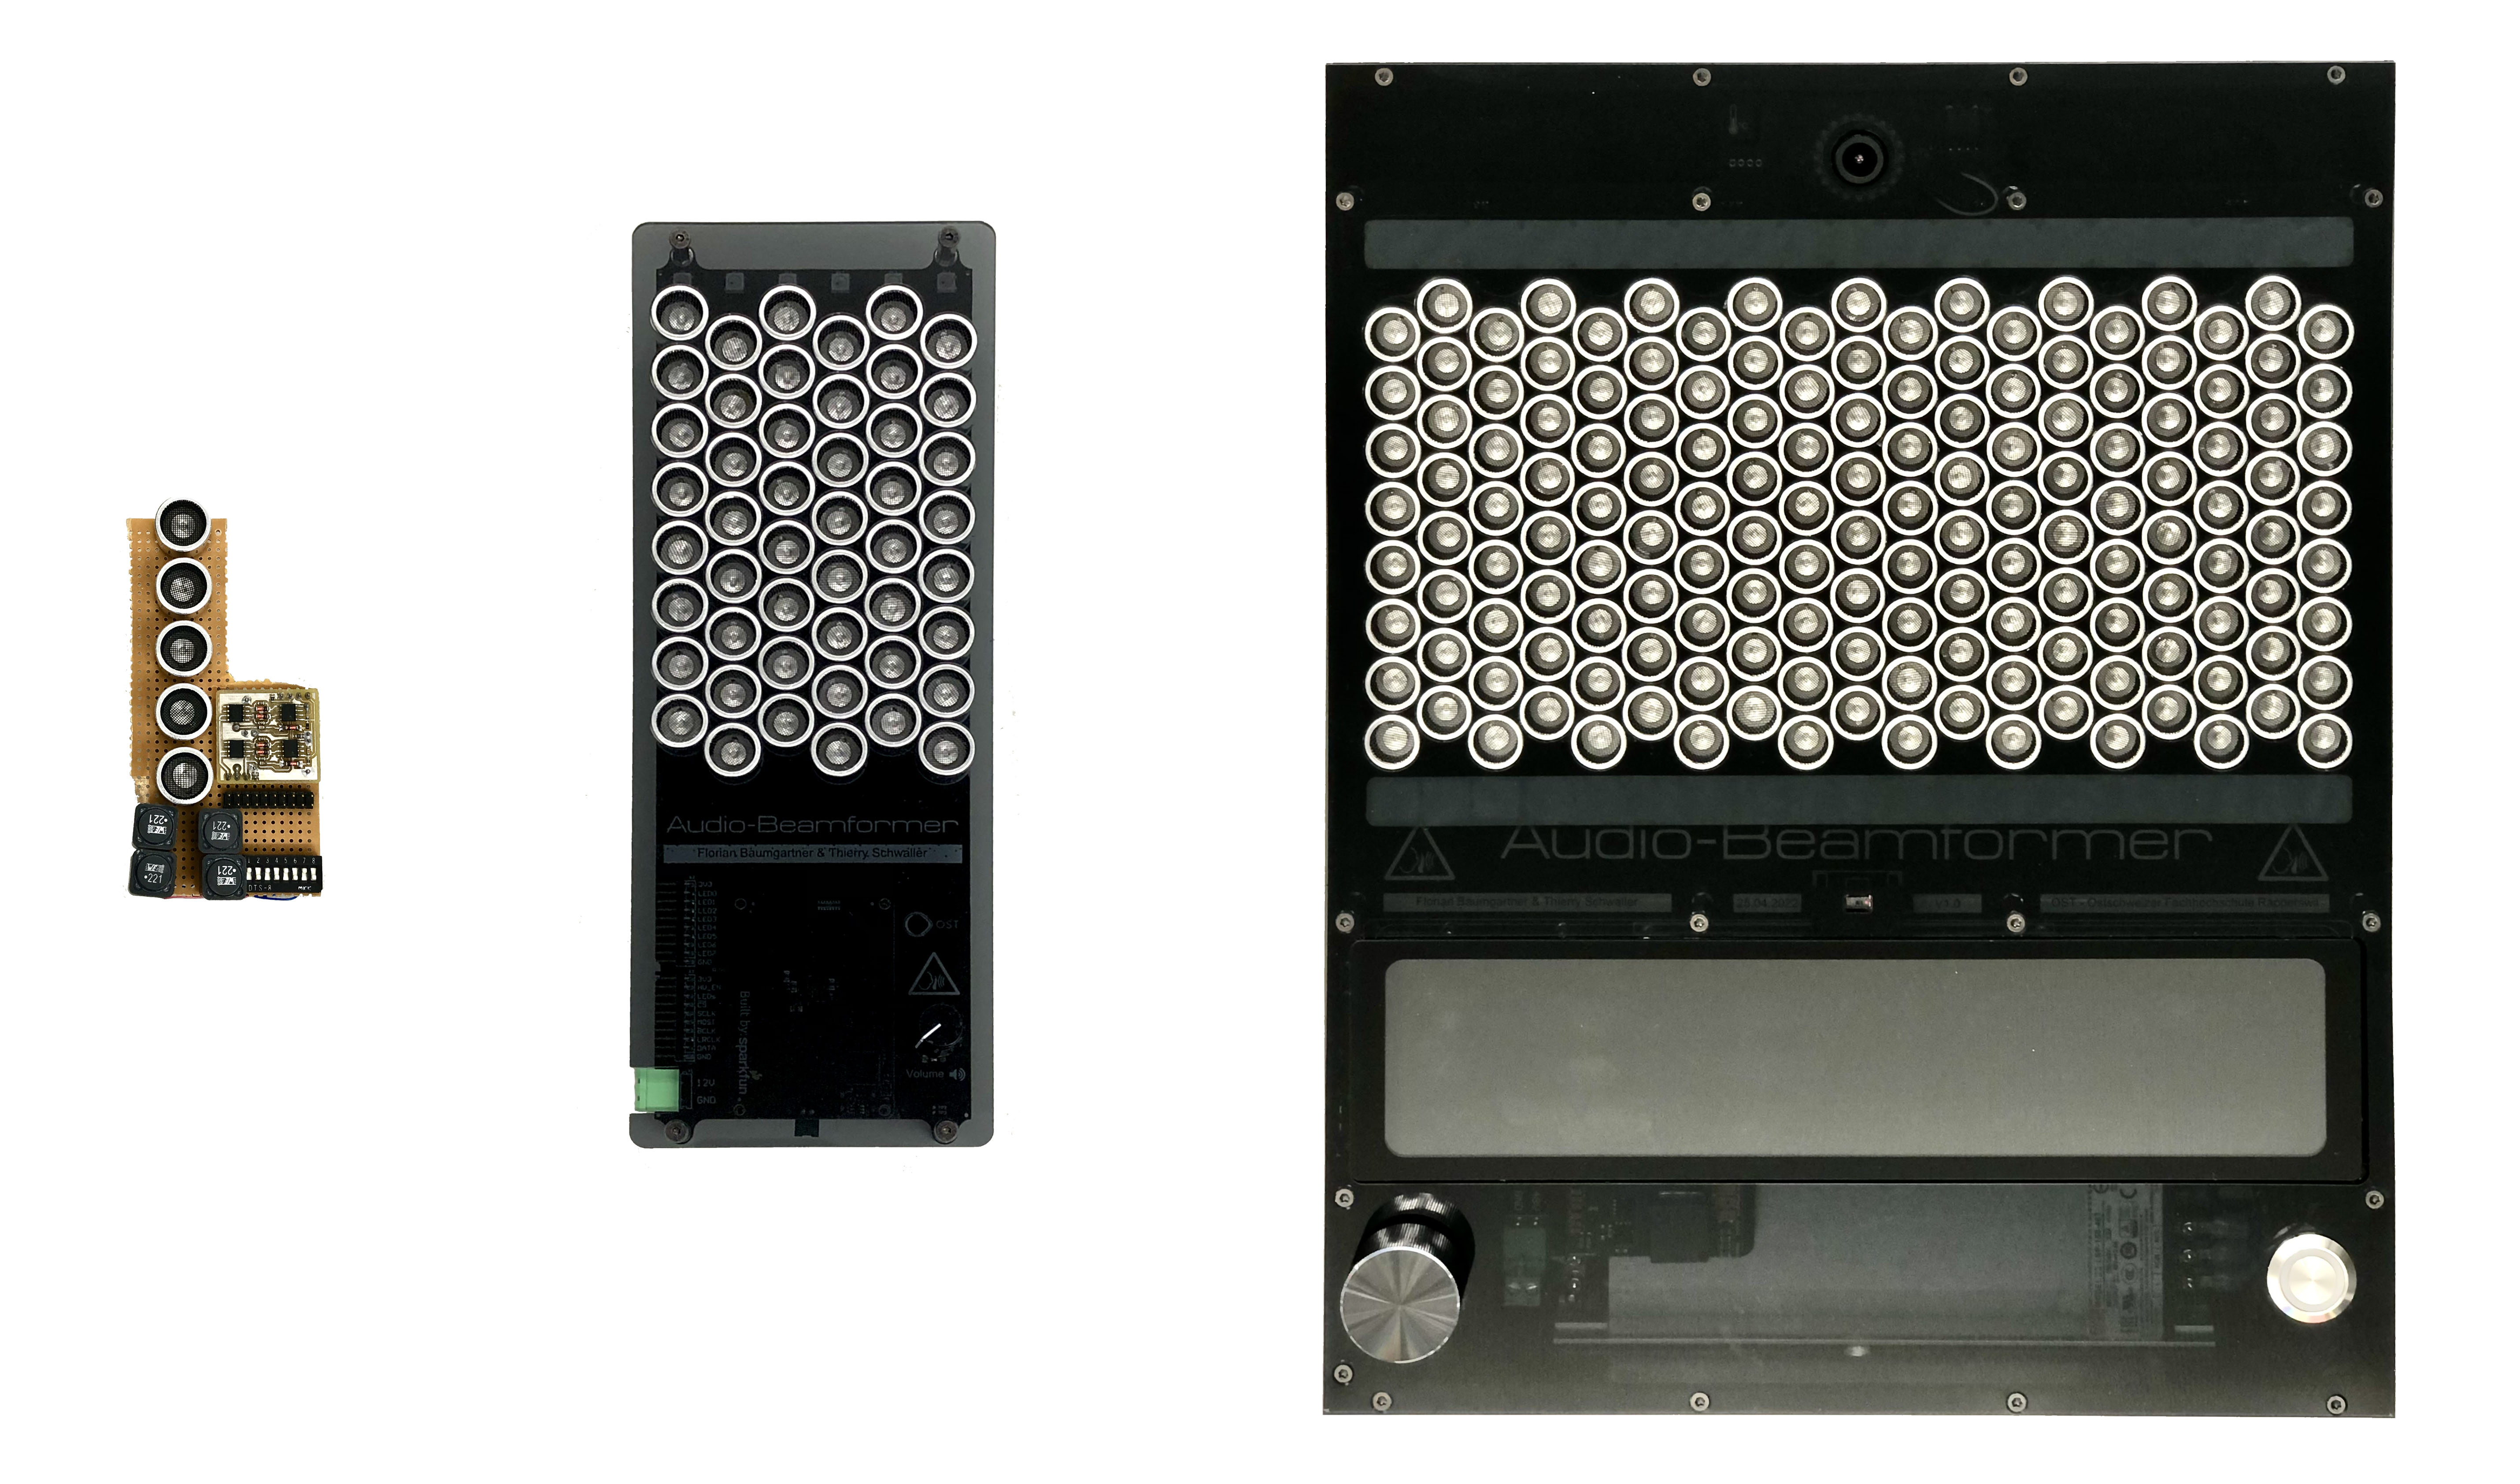
\includegraphics[width=\textwidth]{images/1_Introduction/Approach.jpg}
	\vspace{-0.4cm}
    \caption{Hardware Prototype Revisions}
    \label{fig:prototype_revisions}
\end{figure}


\section{Open Source}
Right from the start it was decided that everything about the project would be released under an open source license. Both of us are huge supporters of open source and believe it will be the future of engineering. Building upon existing libraries and code under open source licenses, allowed us to accelerate the design process. Sometimes open source is considered an act of charity, but in our case, the benefits of using it outweigh any closed source processes. All documents and files for this project can be found on our GitHub page. A short description of all the repositories can be found in the Appendix \ref{Data Archive}.

\chapter{Requirements Specification and Project Schedule}
%\clearpage
\newpage

\section{Requirements Specification} \label{Requirements Specification}
\enlargethispage{2.5cm}
\begin{adjustwidth}{0.23cm}{0cm} \hfuzz=7.0pt \vfuzz=19.0pt
\makebox[\textwidth]{\frame{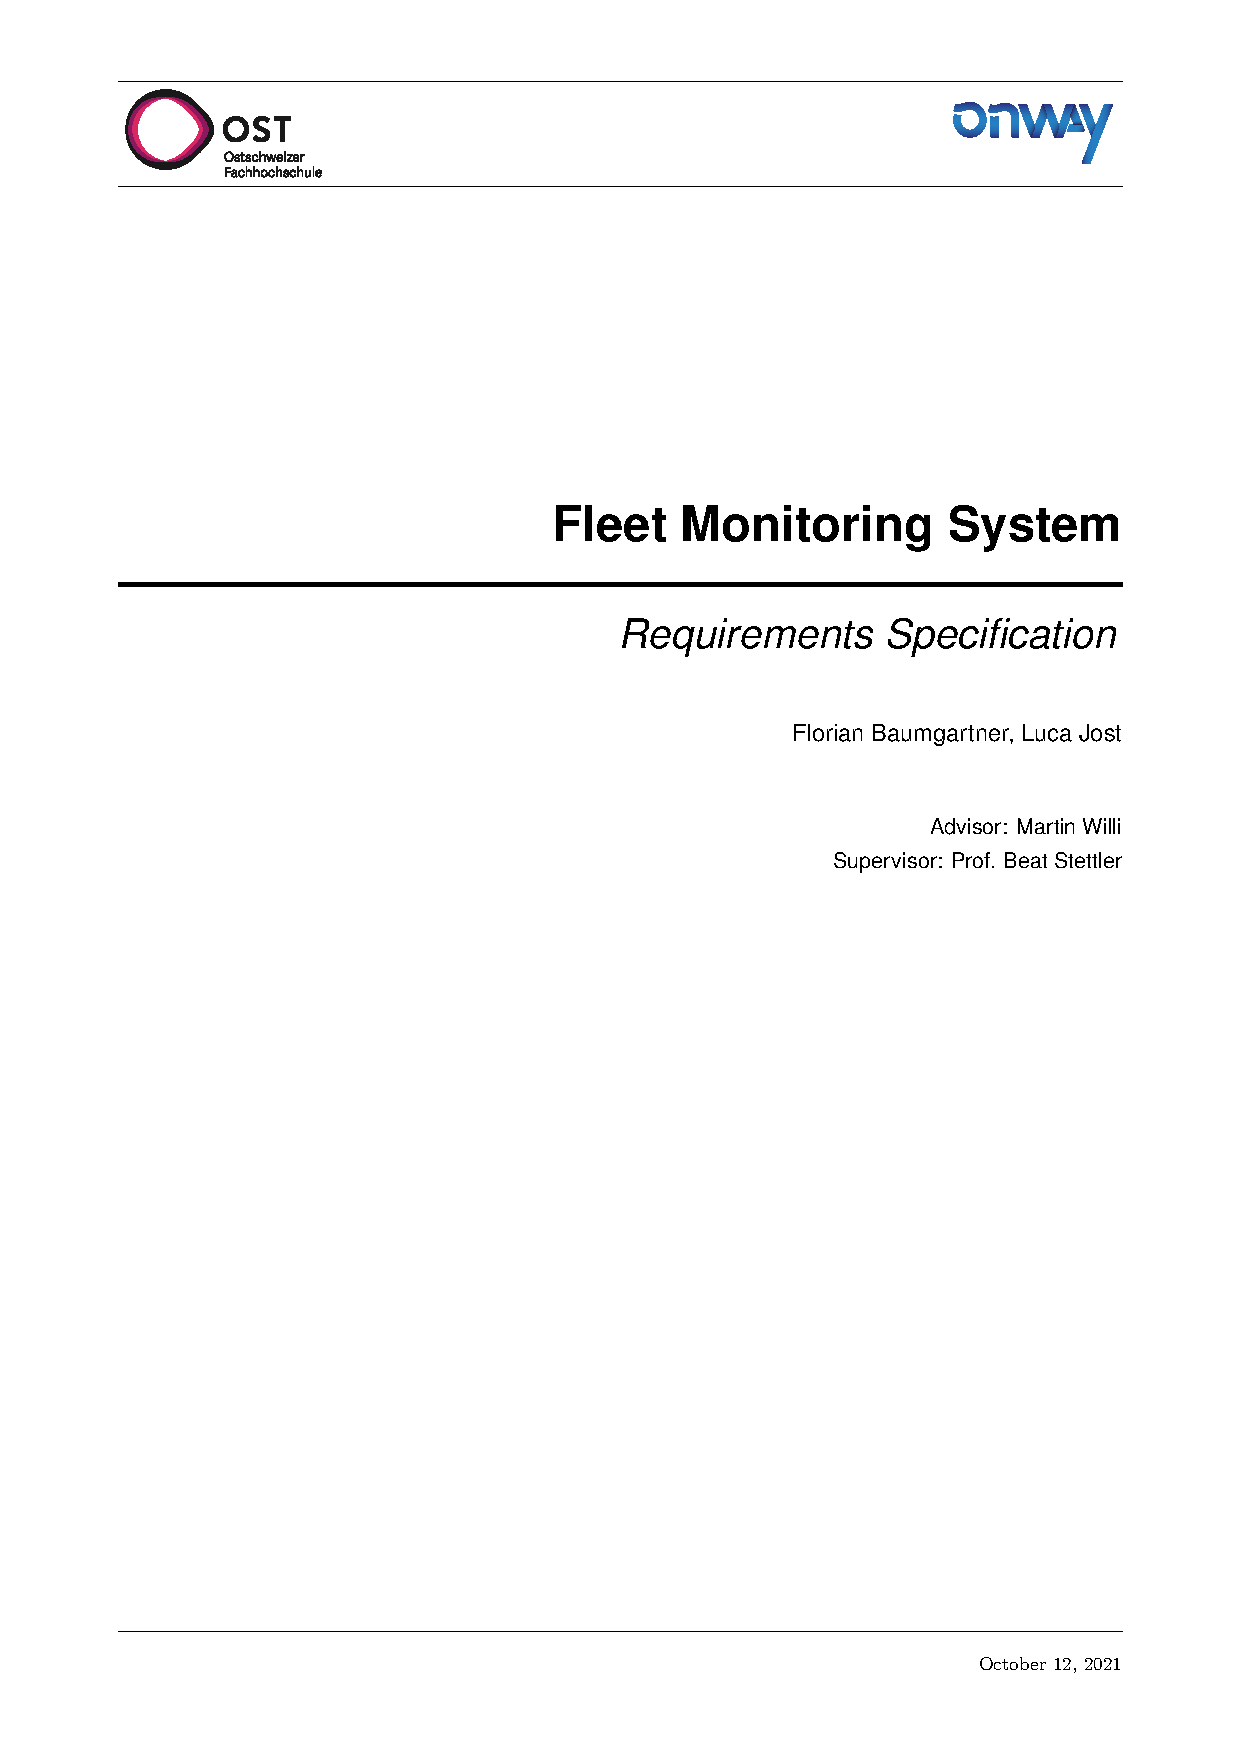
\includegraphics[width=17.3cm, page=1]{appendix/Requirements_Specification}}}
\end{adjustwidth}
\newpage

\begin{adjustwidth}{-0.23cm}{0cm} \hfuzz=7.0pt \vfuzz=19.0pt
\makebox[\textwidth]{\frame{\includegraphics[width=17.3cm, page=2]{appendix/Requirements_Specification}}}
\end{adjustwidth}
\newpage

\begin{adjustwidth}{0.23cm}{0cm} \hfuzz=7.0pt \vfuzz=19.0pt
\makebox[\textwidth]{\frame{\includegraphics[width=17.3cm, page=3]{appendix/Requirements_Specification}}}
\end{adjustwidth}
\newpage

\begin{adjustwidth}{-0.23cm}{0cm} \hfuzz=7.0pt \vfuzz=19.0pt
\makebox[\textwidth]{\frame{\includegraphics[width=17.3cm, page=4]{appendix/Requirements_Specification}}}
\end{adjustwidth}
\newpage

\begin{adjustwidth}{0.23cm}{0cm} \hfuzz=7.0pt \vfuzz=19.0pt
\makebox[\textwidth]{\frame{\includegraphics[width=17.3cm, page=5]{appendix/Requirements_Specification}}}
\end{adjustwidth}
\newpage

\begin{adjustwidth}{-0.23cm}{0cm} \hfuzz=7.0pt \vfuzz=19.0pt
\makebox[\textwidth]{\frame{\includegraphics[width=17.3cm, page=6]{appendix/Requirements_Specification}}}
\end{adjustwidth}
\newpage

\begin{adjustwidth}{0.23cm}{0cm} \hfuzz=7.0pt \vfuzz=19.0pt
\makebox[\textwidth]{\frame{\includegraphics[width=17.3cm, page=7]{appendix/Requirements_Specification}}}
\end{adjustwidth}
\newpage

\begin{landscape}
    \section{Project Schedule}
    \begin{figure}[h!]
    	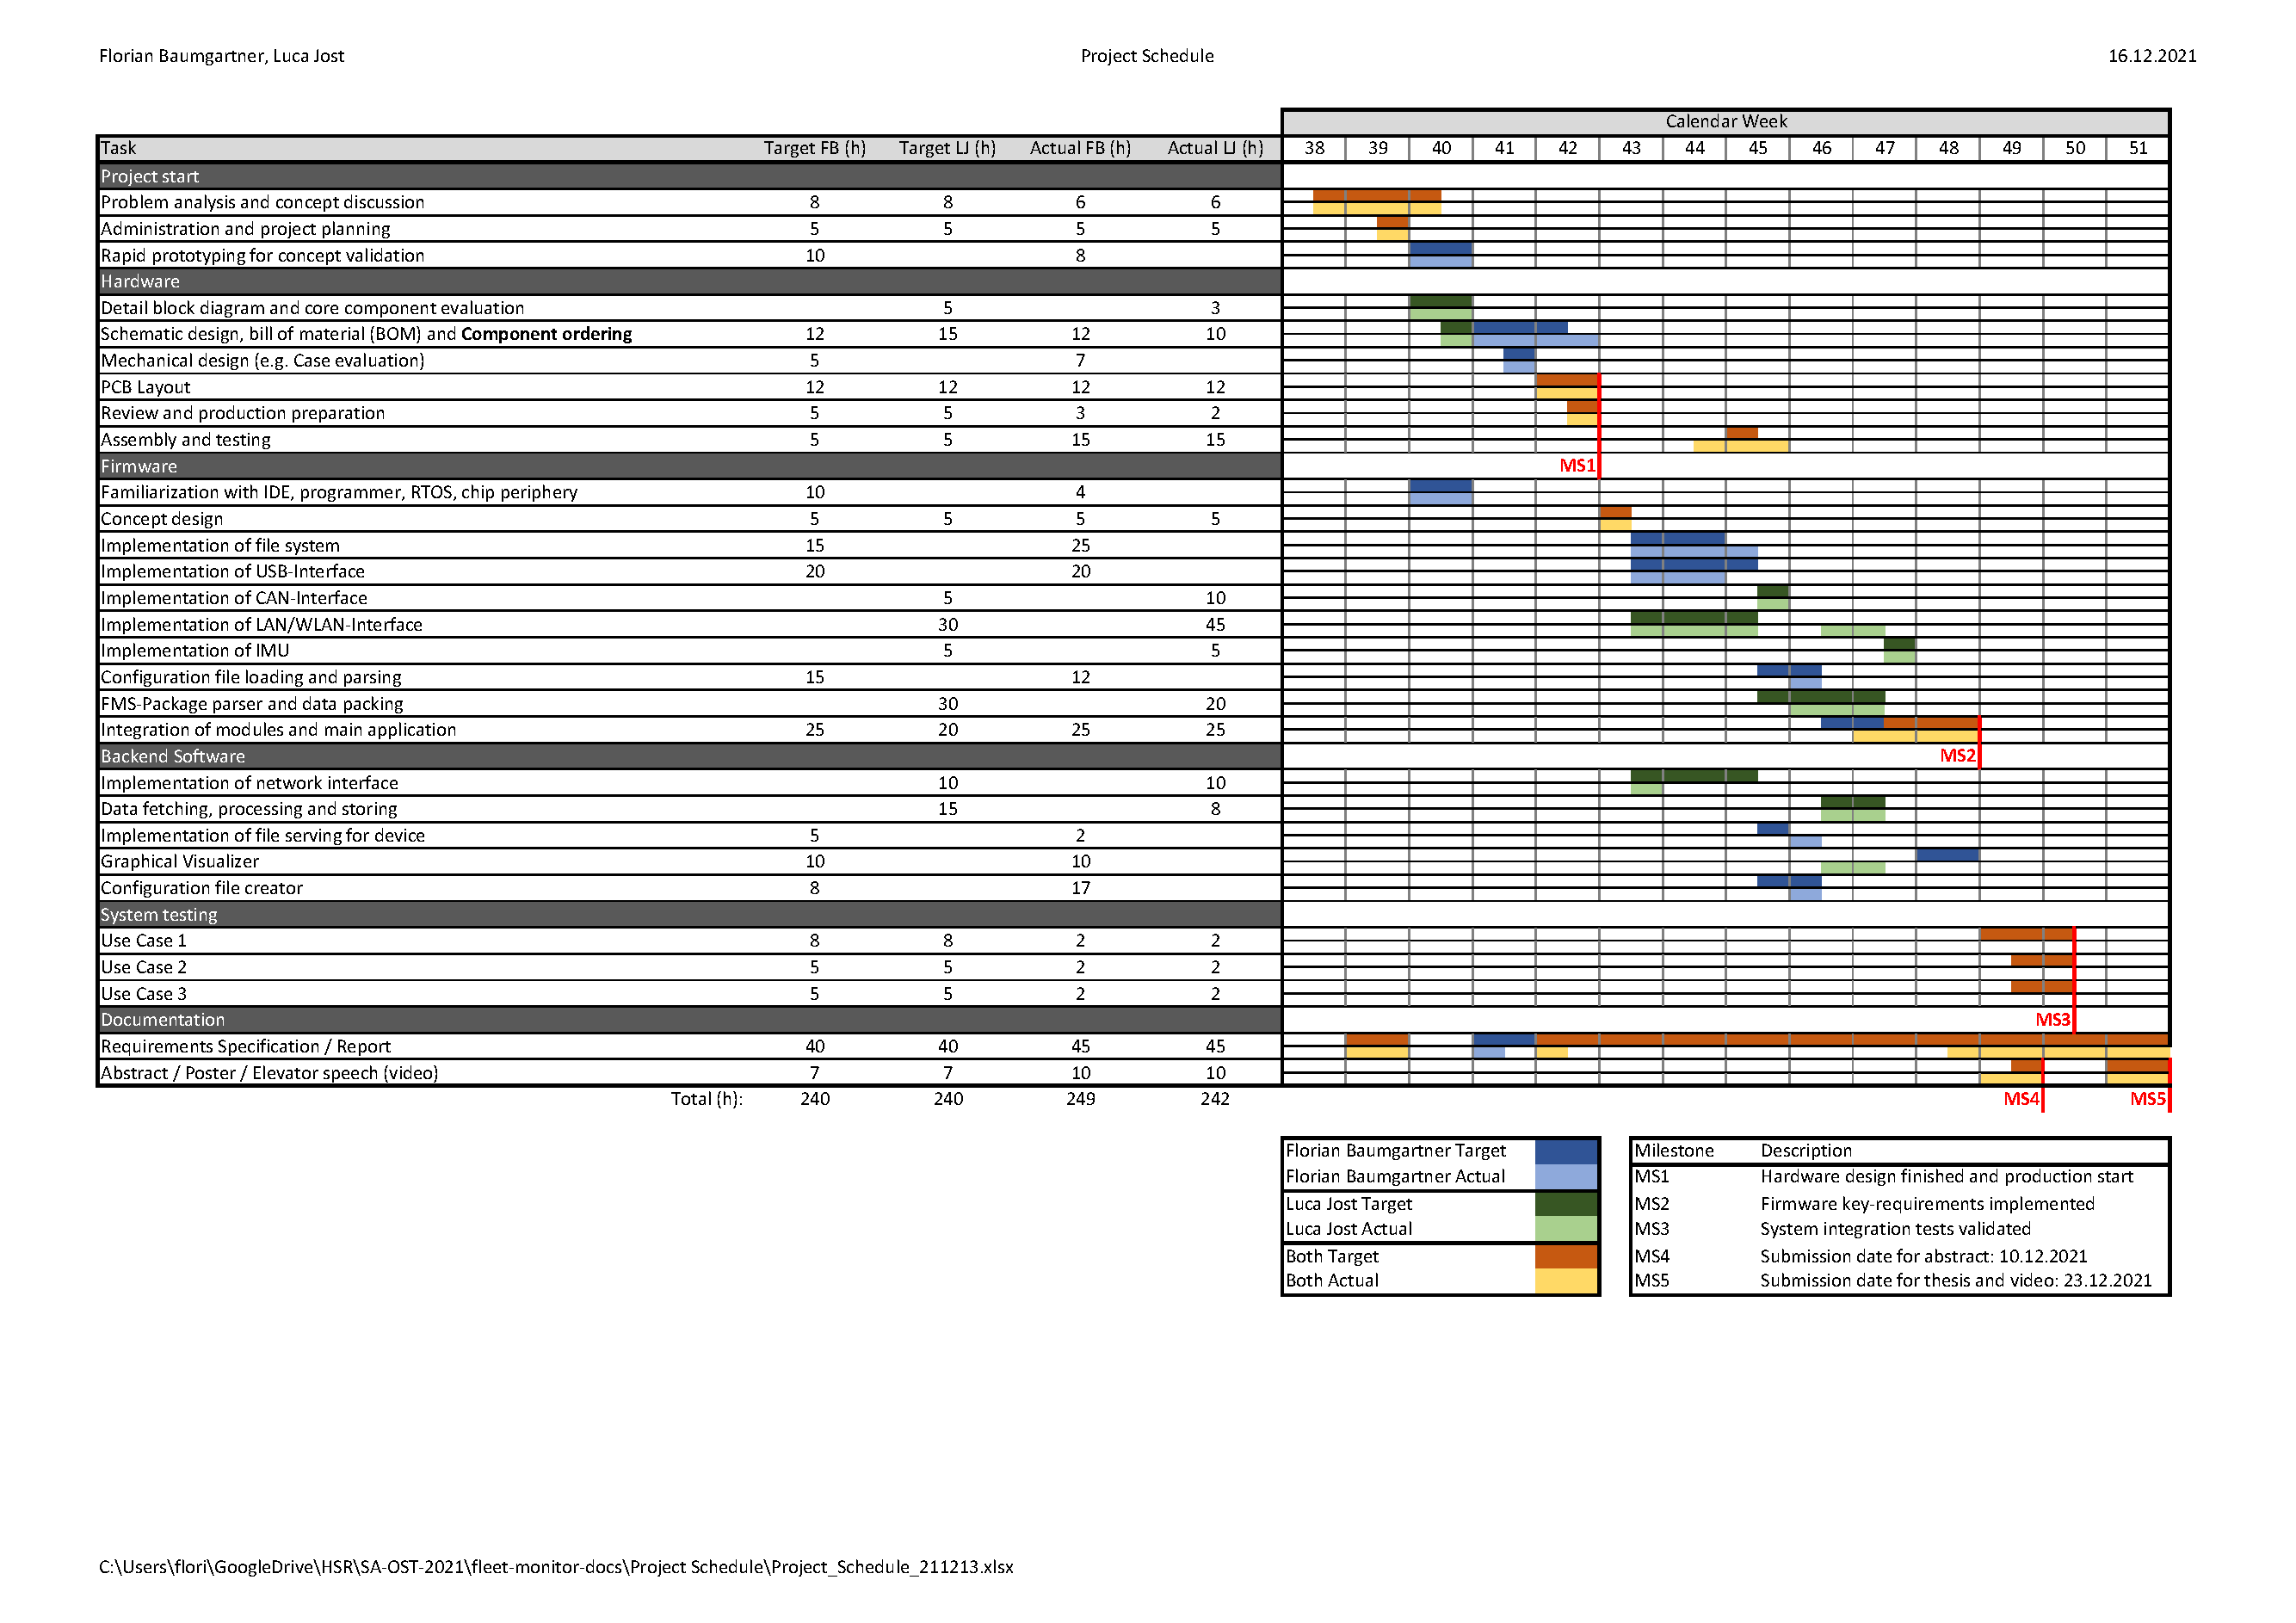
\includegraphics[height=13.4cm, trim=17mm 64mm 24mm 19mm, clip]{appendix/Project_Schedule_211213}
    	\bigskip
    	\caption{Project Schedule}
    	\hfuzz=19.0pt
	    \vspace{-1.5cm}
	    \label{fig:project_schedule}
    \end{figure}
\end{landscape}
\newpage
\addtolength{\textheight}{\topskip}
\chapter{Preliminaries}
\section{Controller Area Network (CAN)}
\subsection{Basics}
\acrshort{iso}11898 describes the physical data link layer implementation of \acrshort{can}. This specification describes a twisted-wire pair bus with 120\,$\Omega$ line impedance, and differential signaling at a rate up to 1\,Mbit/s. A network is constructed with two or more transceivers on the same bus lines. The network must be terminated with a 120\,$\Omega$ resistor at each end of the bus, as shown in Figure \ref{fig:can-bus_topology}.

\begin{figure}[h!]
	\centering
	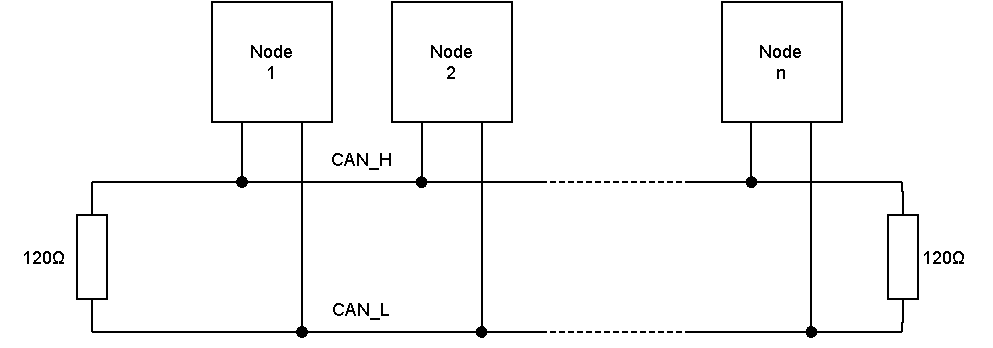
\includegraphics[height=3.8cm]{images/can-bus_topology}
	\caption{Topology of a \acrshort{can}-Bus}
	\label{fig:can-bus_topology}
\end{figure}

As long as the bus is free, any node is allowed to transmit \acrshort{can} messages. Each message is received by all nodes on the network, including the node that sent the message. This type of data broadcasting allows multiple nodes to use the transmitted data. It also allows the sending node to monitor the bus for errors. If two or more nodes try to transmit at the same time, the lower priority message will be overwritten, and this lower priority node will halt transmission upon sensing overwritten bits in its message identifier. The message is then re-transmitted when the bus is free again. This non-destructive process is called bit-wise arbitration.

Every node on the network reads the identifier of a message, and each node independently determines if the message is to be ignored or processed. Since the identifier is specific to the contents of the message rather than the identity of the originating node, new nodes may be added to the network, without modifying the firmware of any existing node on the network \cite{ti_can_transceivers}.
\newpage

\subsection{Signaling}
The signals on the \acrshort{can} bus are distinguished between two bus logic states, dominant and recessive. A recessive bit is defined as CANH being less than CANL + 0.5\,V. A dominant bit is defined as CANH being more than CANL + 0.9\,V. Figure\,\ref{fig:can-signaling} illustrates the nominal case. Since dominant bits overwrite recessive bits, \acrshort{can} manages message collision through the process of bit-wise arbitration as described earlier.

\begin{figure}[h!]
	\centering
	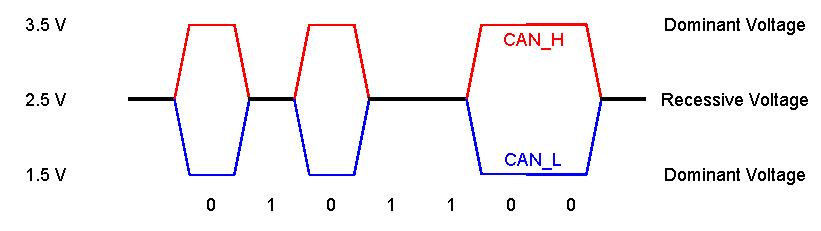
\includegraphics[height=3cm]{images/can-signaling}
	\caption{\acrshort{can}-Bus Signaling}
	\label{fig:can-signaling}
\end{figure}

\subsection{Frames}
Messages over a \acrshort{can} bus are referred to as frames. The most common frame types are defined as \acrshort{can} 2.0A and 2.0B also known as base and extended frame. 2.0A is simply a \acrshort{can} frame with an 11-bit identifier and 2.0B always uses 29-bit. A \acrshort{can} frame is always split up into the following regions \cite{can_bus_tutorial}.

\begin{figure}[h!]
	\centering
	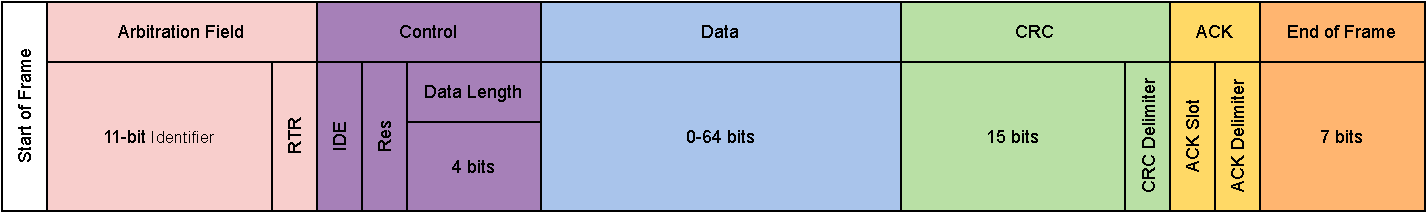
\includegraphics[width=\textwidth]{images/can-frame}
	\caption{Base 11-bit identifier \acrshort{can} frame}
	\label{fig:can-frame}
\end{figure}

\begin{itemize}
		\item The Arbitration Field, includes the identifier of the message and defines the priority. The identifier must be 11 or 29 bits long. Also in this field is the \acrfull{rtr} bit, which is used to request data.
		\item The Control Field is used to differentiate between the two frame types and defines the incoming data length.
		\item The data field can contain 0-8 bytes of information.
		\item The \acrshort{crc} field contains a 15-bit checksum. The checksum is used to detect errors in the transmission.
		\item The Acknowledgement Slot, is used to detect if a message was received by any of the devices on the bus. The transmitter checks for the presence of the Acknowledge bit and re-transmits the message if no acknowledge was detected.
\end{itemize}
\newpage

\section{SAE J1939}
J1939 is the open standard developed by \acrfull{sae}. It is used for networking and communication in the commercial vehicle sector. J1939 is a higher-layer protocol utilizing \acrshort{can} as its physical layer. \acrshort{sae}\;J1939 is primarily a data-driven protocol, providing far better data bandwidth than other automation protocols such as \gls{canopen} and \gls{devicenet} \cite{introduction_sae_j1939_protocol}.

The standard specifies \acrshort{can} bus speeds of 250\,kbit/s or 500\,kbit/s and uses the extended 29-bit identifier frame format. Most messages defined by the J1939 standard are intended to be broadcast only. This means that the data is transmitted on the network without a specific destination. This permits any device to use the data without requiring additional request messages. The 29-bit identifier used in J1939 is structured in the following way \cite{sae_j1939_introduction}. 

\begin{figure}[h!]
	\centering
	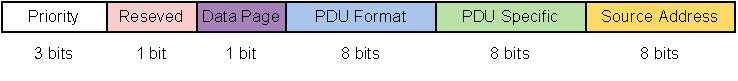
\includegraphics[width=\textwidth]{images/j1939-identifier}
	\caption{29-bit J1939 Identifier}
	\label{fig:29-bit_J1939_Identifier}
\end{figure}
\begin{itemize}
	\item The first three bits of the identifier are used for controlling a message priority during the arbitration process. A value of 0 has the highest priority.
	\item The Reserved bit, Data Page bit, \acrfull{pdu} Format field and \acrshort{pdu} specific field are often grouped together and referred as \acrfull{pgn}. 
	\item The last 8 bits of the identifier contain the address of the device transmitting the message. Two devices can not share the same address.
\end{itemize}
\newpage

\section{Fleet Management System (FMS)} \label{Fleet Management System (FMS)}
The \acrfull{fms} Interface is a standard interface developed by European commercial vehicle manufacturers in 2002. It defines a common interface for telematics applications and includes driving as well as diagnostics information. The data is coded according to the \acrshort{sae}\,J1939 standard. \acrshort{fms} is a broadcast-only system, a gateway between the internal bus and the \acrshort{fms} bus is implemented by the \acrshort{oem}. third party systems, like the Fleet-Monitor, are forbidden on the internal bus as shown in figure \ref{fig:fms-bus}. 

\begin{figure}[h!]
	\centering
	\hfuzz=14.0pt
	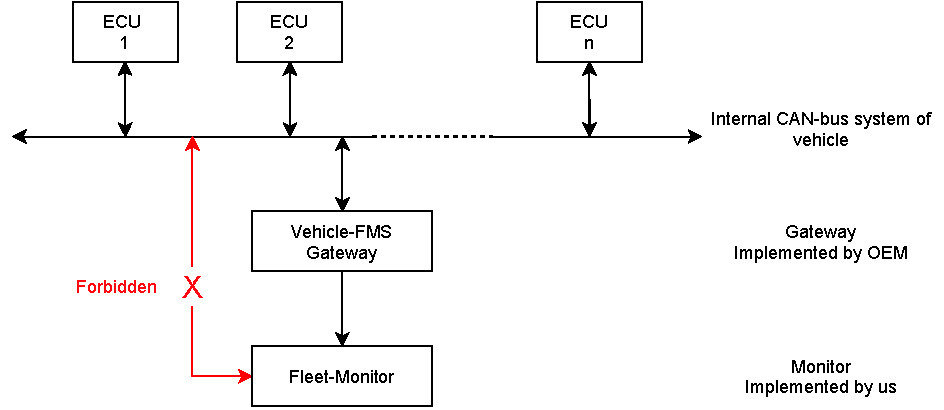
\includegraphics[width=\textwidth]{images/fms-bus}
	\vspace{-0.2cm}
	\caption{FMS Topology}
	\label{fig:fms-bus}
\end{figure}

At the time of writing, the standard includes 35 different packages, ranging from engine coolant temperature to door position.  Depending on the frame, updates occur between 20\,ms and 10\,s. The convention set the \acrfull{pgn} for J1939 identifiers, while the \acrshort{oem} specifies the source address and priority. Each frame has a fixed data length of 8\,byte but not all of them contain information as shown in the example frame below.\cite{fms-standard-description}

\begin{figure}[h!]
	\centering
	\hfuzz=11.0pt
	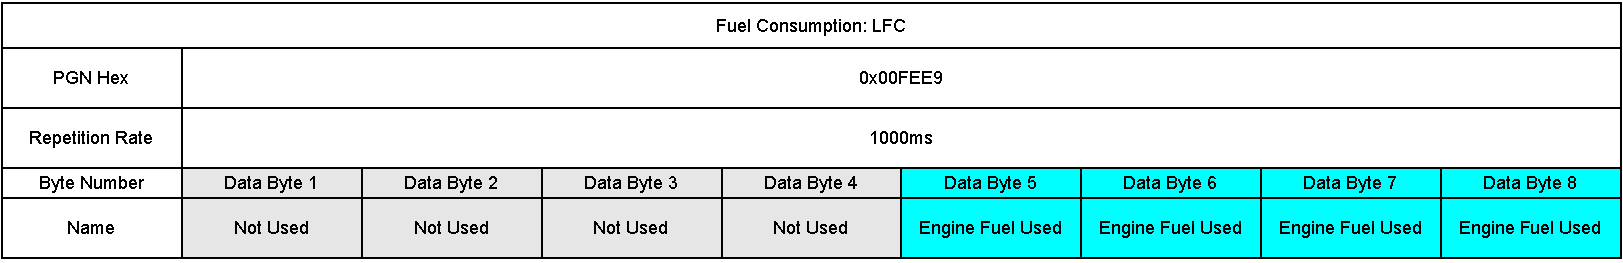
\includegraphics[width=\textwidth]{images/fms-frame}
	\caption{Fuel Consumption FMS Frame}
	\label{fig:fms-frame}
\end{figure}


\chapter{Development}

%% Section Hardware Design %%
\section{Hardware Design}
The hardware of the Fleet-Monitor was designed using Altium Designer 21. The integrated 3D \acrshort{cad} functionality simplified the overall development and lowered the possibility of errors in the design. The 4-Layer \acrfull{pcb} with the size of 140.5\,mm\;x\;79.5\,mm has been manufactured and assembled by JLCPCB.\newline
As a proof of concept, five prototypes have been made, which are all fully tested and in working condition.

\begin{figure}[h!]
	\hfuzz=57.0pt
	\hspace{-1.4cm}
	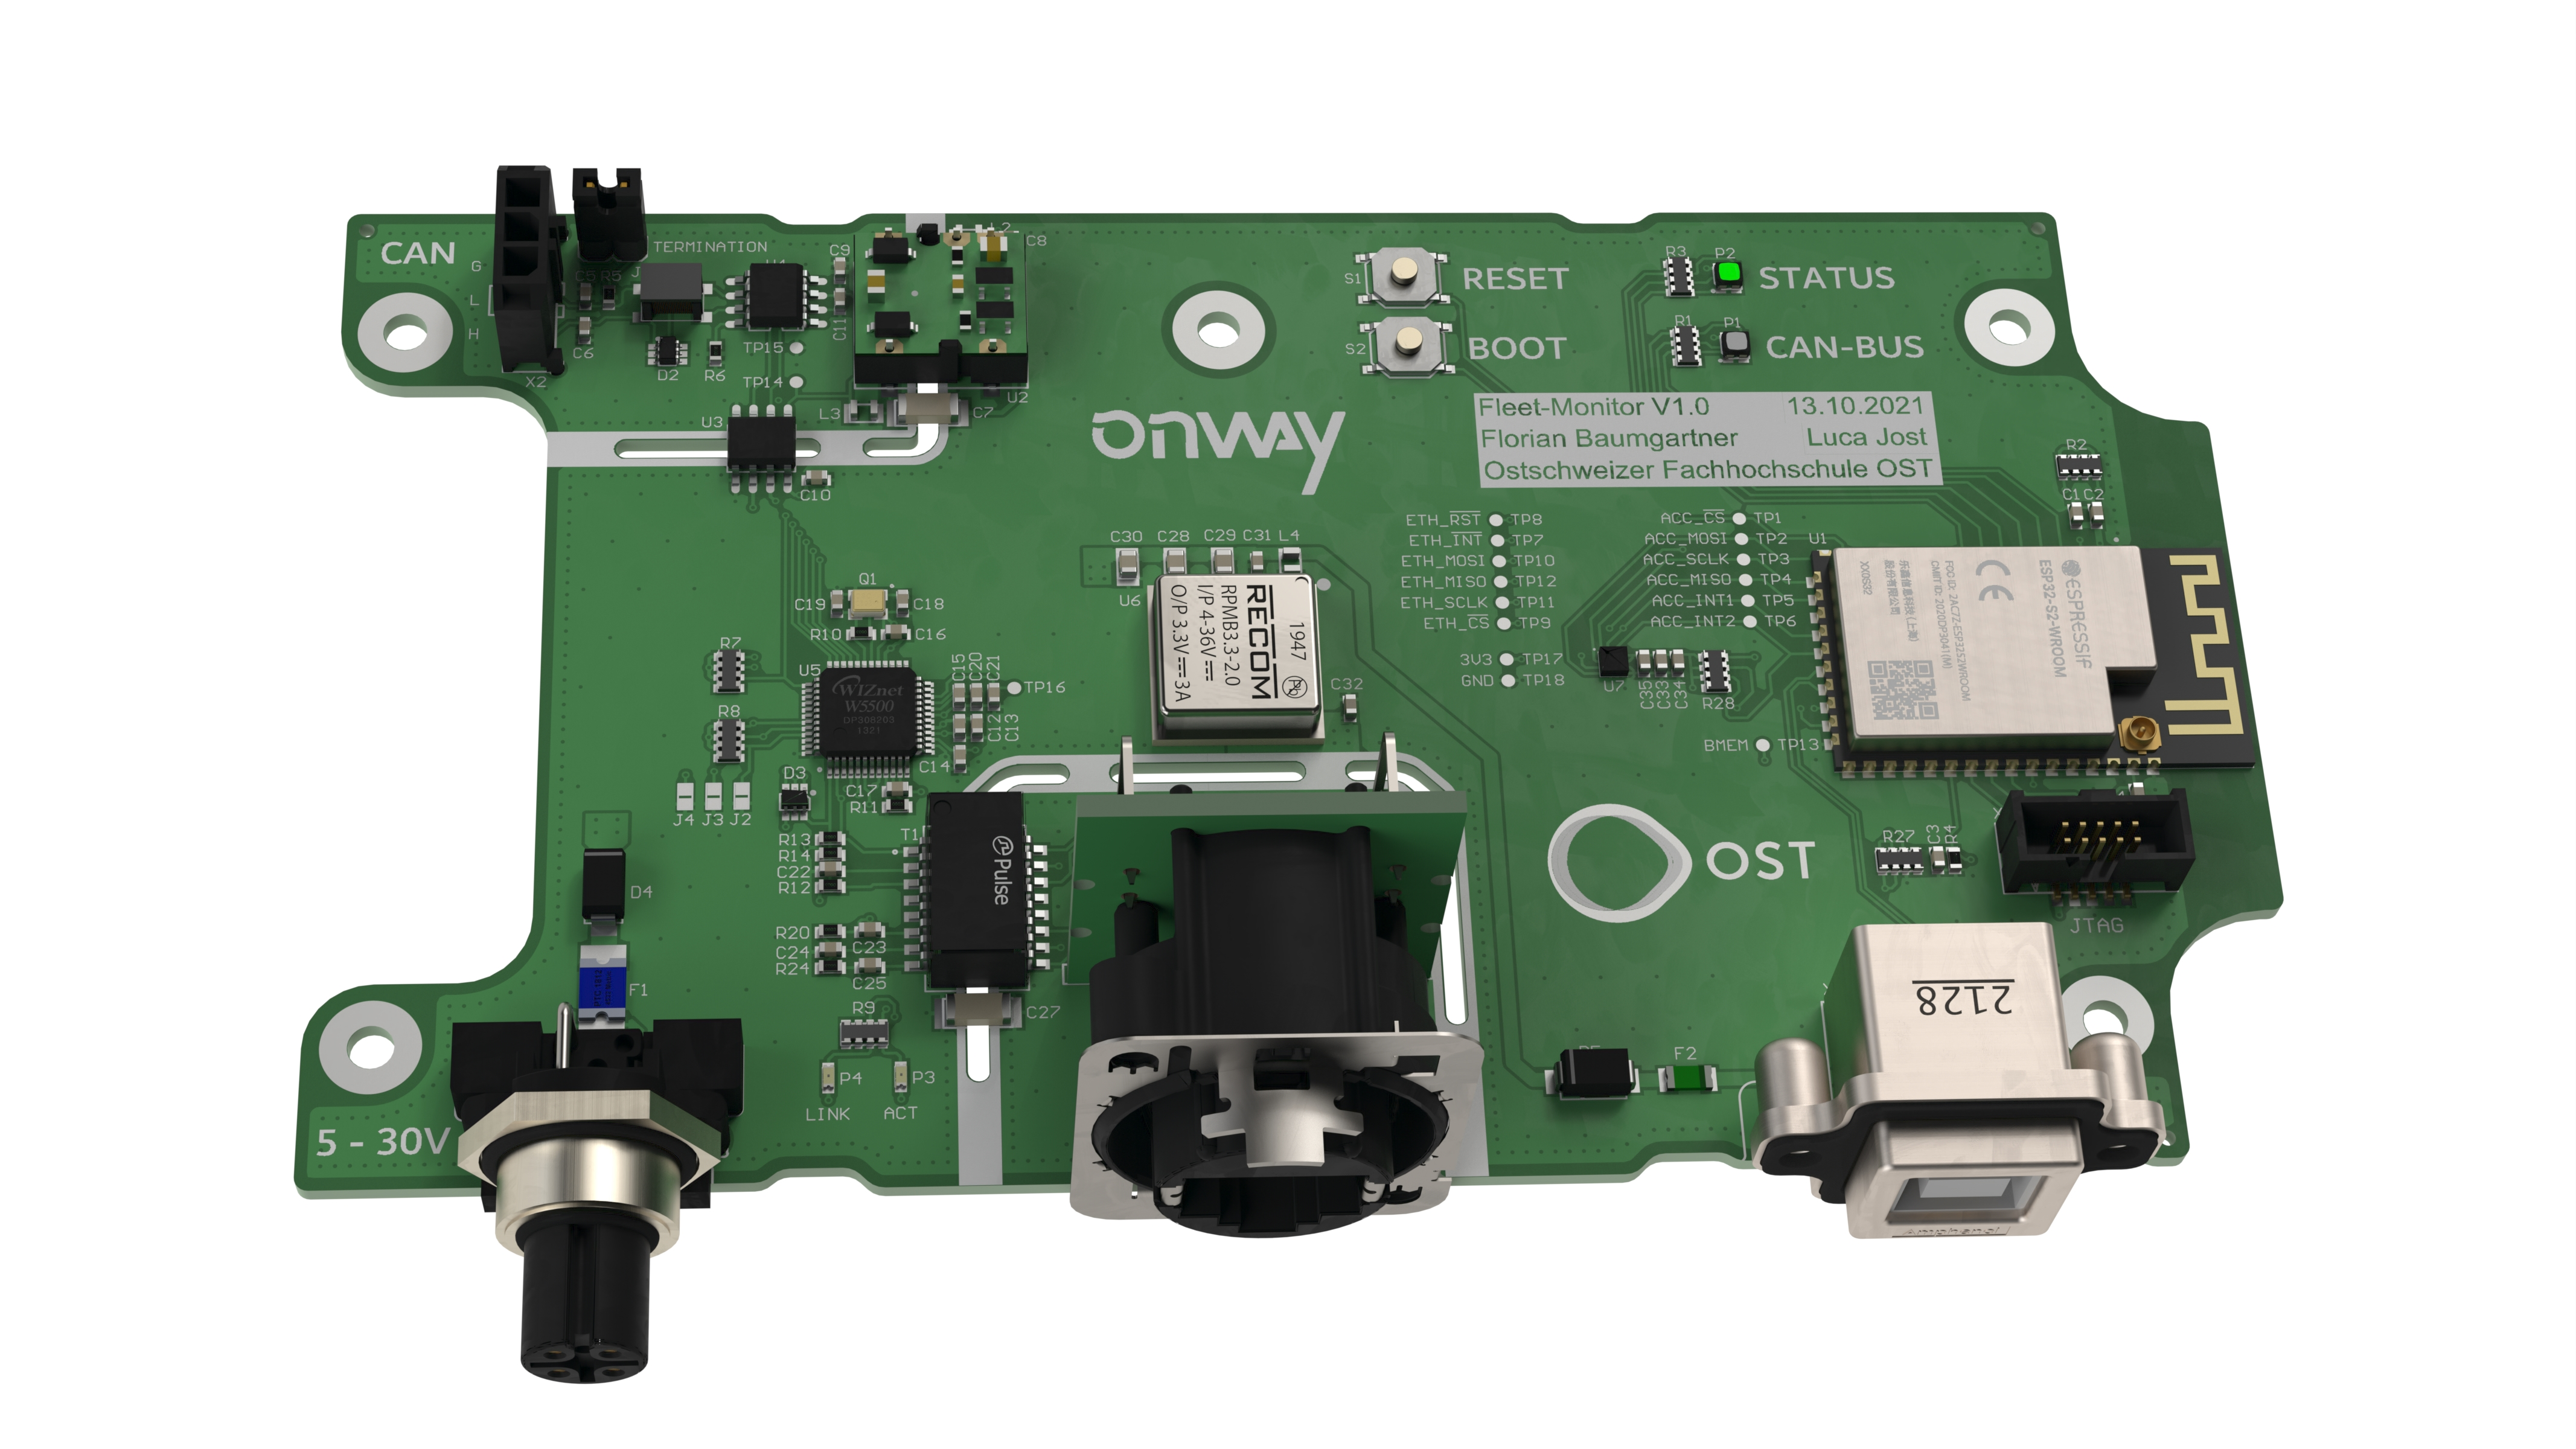
\includegraphics[height=10.0cm]{images/fleet-monitor-rendering-pcb}
	\caption{Assembled PCB 3D-Render}
	\label{fig:fleet-monitor-rendering-pcb}
\end{figure}
\newpage

\subsection{Block Diagram}
The hardware block diagram in Figure \ref{fig:hardware-block-diagram} offers an overview of the system architecture.

\medskip
\begin{figure}[h!]
	\centering
	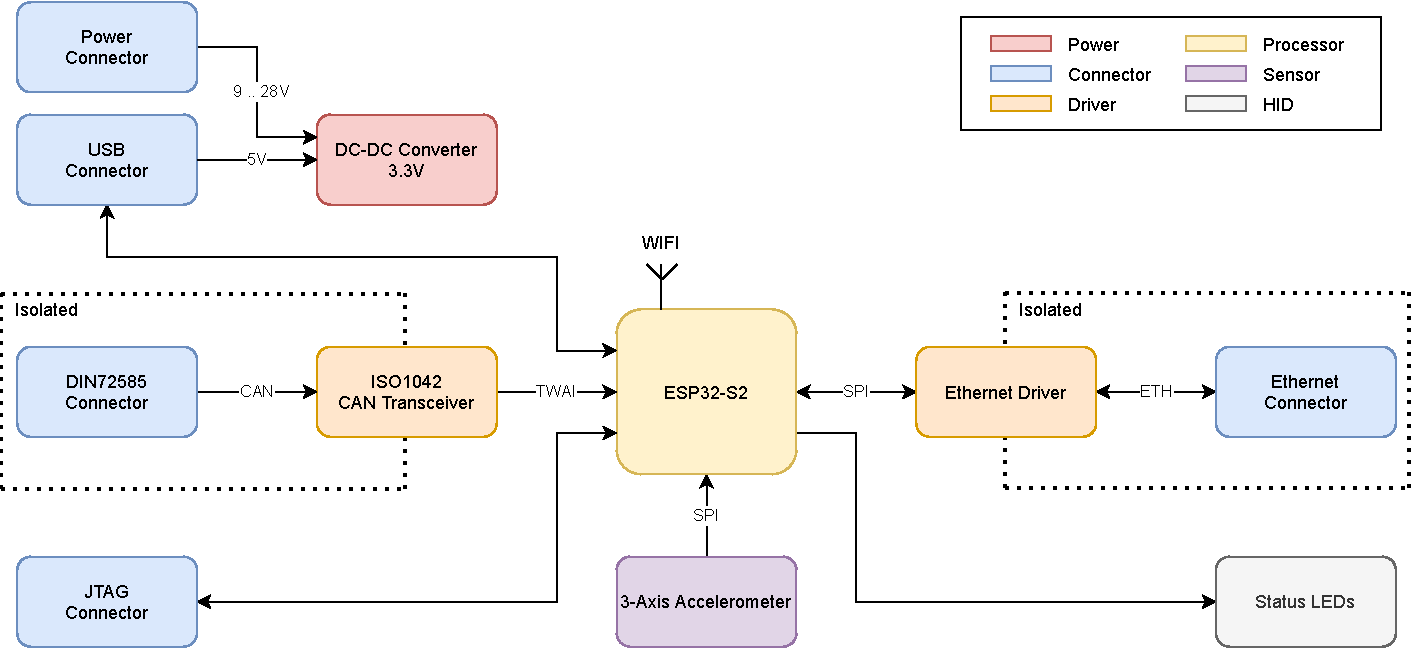
\includegraphics[width=\textwidth]{images/fleet_monitor_hardware}
	\vspace{0.1cm}
	\caption{Hardware Block Diagram}
	\label{fig:hardware-block-diagram}
\end{figure}

\subsection{Power Management}
The device can be powered either by the \acrshort{usb}-interface or an external \acrshort{dc} power source. Both supply options are internally connected through Schottky diodes and provide a seamless switch-over. If both supply sources provide power at the same time, the external \acrshort{dc} source is used.\newline
The \acrfull{usb} Interface fulfills all guidelines of the \acrshort{usb} specifications in terms of power consumption. Therefore it is guaranteed, that the maximum current of 500\,mA is not exceeded. In case of failure, a resettable \acrshort{ptc} Poly-fuse protects the power source from over current.\newline
The external power source accepts a voltage range from 9\,V to 28\,V and is protected against reverse polarization and short circuit. As a suitable connector, the industry-standard M12\;(5\;Pin) type has been chosen. It fulfills the IP67 rating and is highly robust against accidental disconnection due to its threaded coupling. In addition, it is used in a wide variety of applications, resulting in great availability. The pin-out consists of pin 1 and 2 used for the positive input and pins 3 to 5 for ground. This has the advantage, that matching connectors with a different amount of pins (e.g. 2-pin connector) can be used as well.

\begin{wrapfigure}{r}{7.5cm}
\vspace{-0.6cm}
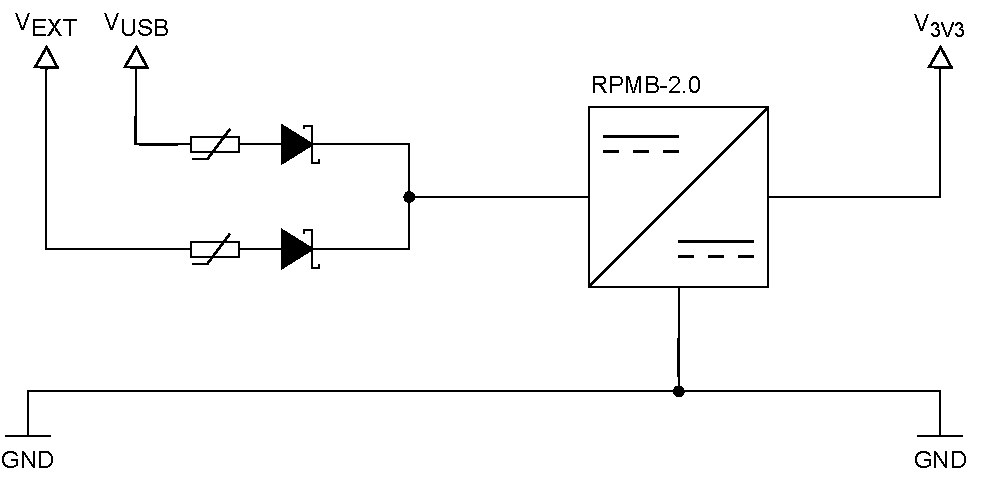
\includegraphics[width=7.5cm]{images/power}
\vspace{-0.4cm}
\caption{Simplified Power Management}
\label{fig:simplified-power}
\end{wrapfigure} 
The core of the power management unit is based on a Recom \acrshort{dc}/\acrshort{dc} converter of the RPMB-2.0 series. The very compact design, great performance and fairly low price offers an optimal solution. The internal system supply voltage is 3.3\,V and the total power consumption of the device is on average around 1.5\,W.
\clearpage

\subsection{ESP32-S2} \label{ESP32-S2}
The choice of a suitable microcontroller is crucial in the design of an embedded system. Several factors were carefully considered and key requirements have been set, such as:

\begin{itemize}
		\item Integrated WiFi subsystem and \acrshort{rf} front-end
		\item System performance: \acrshort{cpu} speed, memory and peripherals
		\item Native \acrshort{usb} 2.0 Interface
		\item Physical package and pin count
		\item Availability (especially in an ongoing worldwide chip-shortage)
\end{itemize}

The Espressif's \gls{esp32} \acrfull{soc} family satisfies all listed requirements and is in addition advertised as a low cost solution.\newline
To reduce design complexity and production cost, the \gls{esp32}-S2 has been embedded as a solder-on module of the type \gls{esp32}-S2-WROOM-I. This module has the advantage of containing the \acrshort{rf} front-end inclusive an integrated \acrshort{pcb} antenna as well as a 4\,MB \acrshort{spi} flash chip.

\begin{figure}[h!]
	\centering
	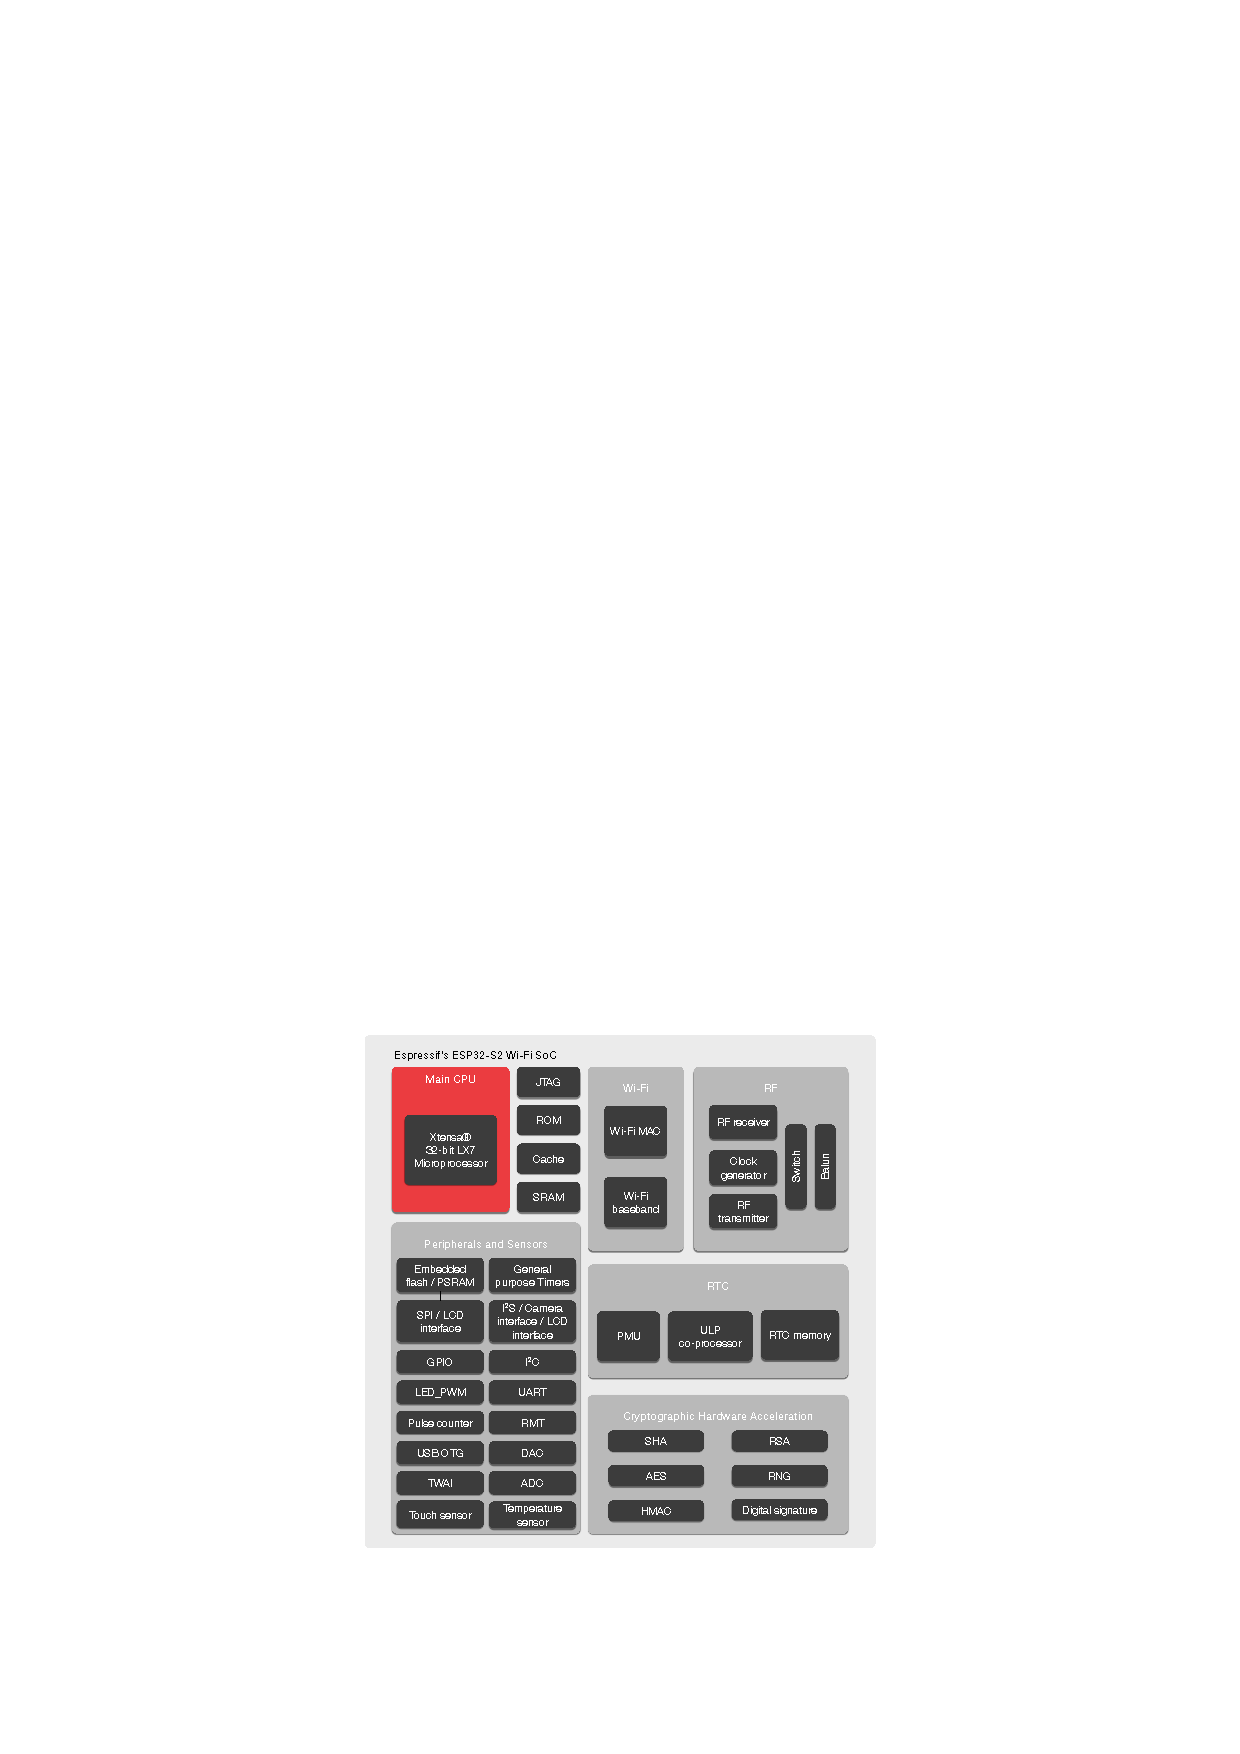
\includegraphics[height=9cm]{images/esp32-s2_block_diagram}
	\caption{ESP32-S2 Block Diagram}
	\vspace{-1.4ex}
	\caption*{\textbf{Source:} ESP32-S2 Datasheet \cite{esp32-s2_datasheet}}
	\label{fig:esp32-s2_block_diagram}
\end{figure}

The \acrshort{soc} can be programmed ether by \acrshort{jtag} and a suitable programmer (e.g. Espressif's \gls{esp32}-Prog) or conveniently over the integrated \acrshort{usb}-Interface.\newline
For uploading code via the \acrshort{usb}-Interface, the \gls{esp32}-S2 has to be set into the device firmware update mode. This can be achieved by pressing the boot button while the device is booting (e.g. after powering on or a reset). If the boot button is not accessible, the user can force the device to enter the \acrshort{dfu} mode by setting a flag in the system configuration. This procedure gets further explained in the user manual \ref{Firmware Update}.
\newpage

\subsection{Ethernet Interface}
In order to connect the device to a host server, an Ethernet interface was added.

\begin{figure}[h!]
	\centering
	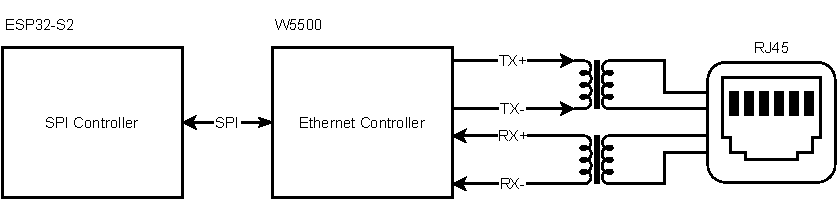
\includegraphics[width=\textwidth]{images/eth_interface}
	\vspace{0.2cm}
	\caption{Simplified Ethernet Interface}
	\label{fig:eth-interface}
\end{figure}

\subsubsection{Controller}
The Ethernet interface utilizes a WIZNet W5500 Ethernet controller chip with an integrated \acrshort{phy} and \acrshort{tcp}/\acrshort{ip} stack. It is capable of transmission speeds of 10 or 100\,MBit/s. The chip is connected through \acrshort{spi} with the main processing unit (\gls{esp32}).

\subsubsection{Isolation}
The \acrshort{ieee} standard 802.3 specifies a 1500\,V\textsubscript{RMS} isolation barrier between the Ethernet \acrshort{phy} Chip and the cable. To comply with these requirements a pulse transformer was used to magnetically couple the data lines between the connector and the chip. Additionally a ground clearance of 3\,mm was chosen to avoid arc-over or tracking between electrical conductors as seen in Figure \ref{fig:eth-pcb}. 

\begin{figure}[h!]
	\centering
	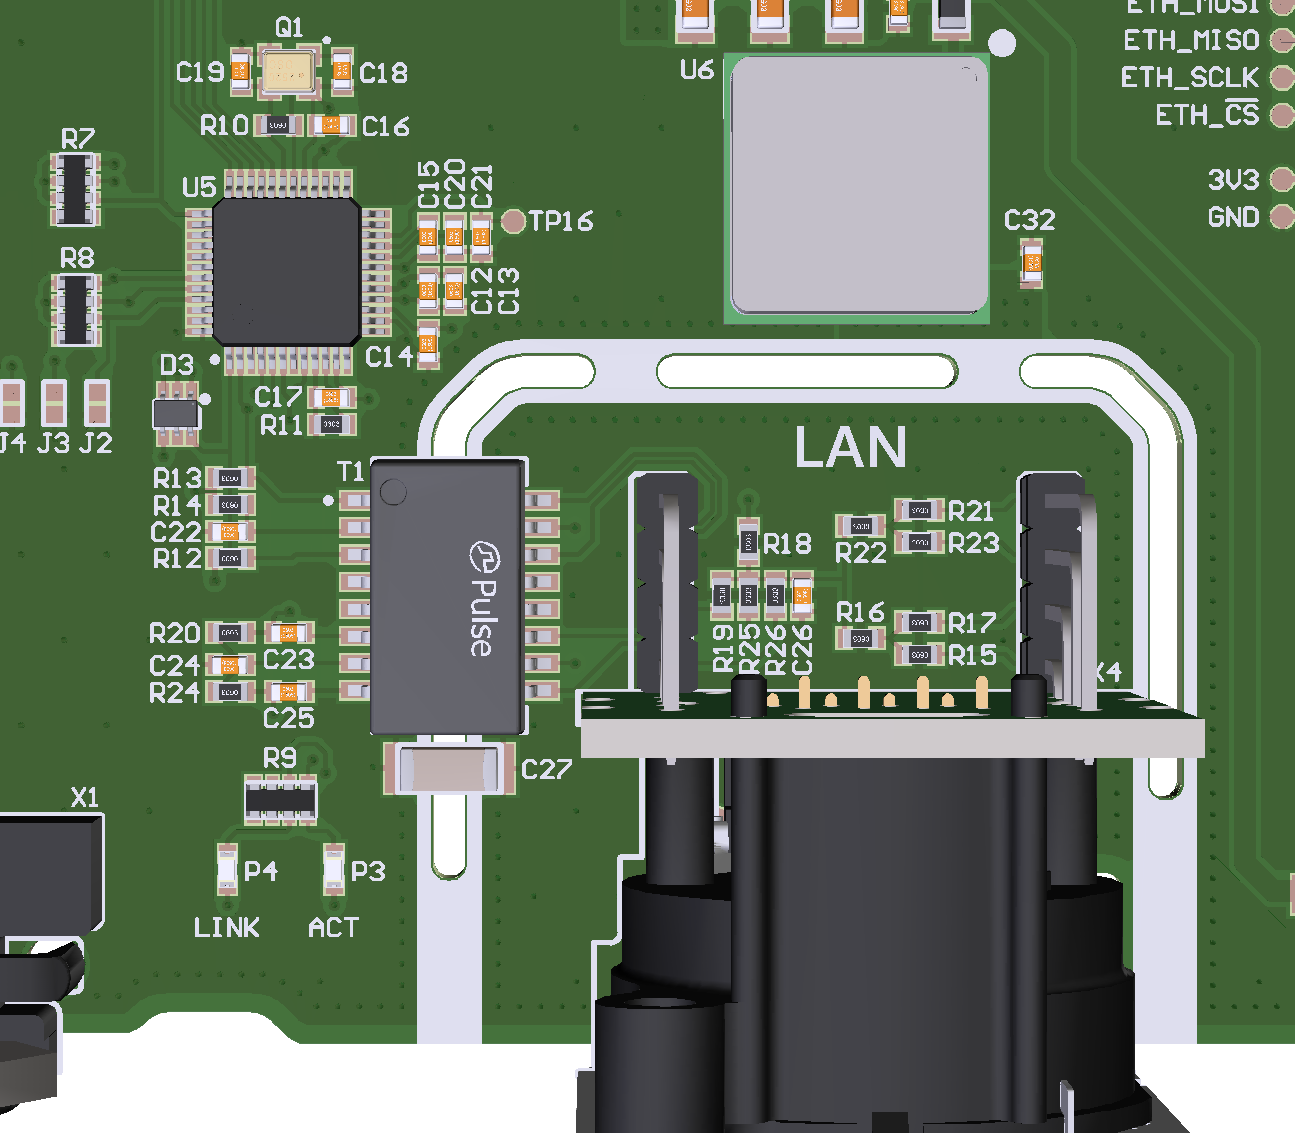
\includegraphics[height=8.5cm]{images/eth-pcb}
	\vspace{0.2cm}
	\caption{PCB view of Ethernet Interface}
	\label{fig:eth-pcb}
\end{figure}
\newpage

\subsubsection{Connector}
The etherCON RJ45 is a lockable connector system, it was chosen for its rugged design and water resistance. This connector system is often used in industrial applications, e.g. in the event industry. The receptacle accepts regular RJ45 plugs as well, but the use of proper etherCON connectors is recommended.

\begin{figure}[h!]
	\centering
	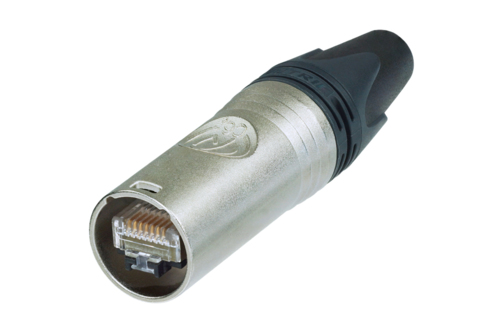
\includegraphics[height=6.5cm]{images/ethercon.jpg}
	\caption{etherCON Connector}
	\vspace{-1.4ex}
	\caption*{\textbf{Source:} Neutrik etherCON Connector NE8MX6 \cite{neutrik-ethercon}}
	\label{fig:neutrik-ethercon}
\end{figure}


\subsection{CAN-Bus Interface}
The \acrfull{twai} is a real-time serial communication protocol suited for automotive and industrial applications. It is compatible with \acrshort{can} bus frames following the \acrshort{iso}-11898-1 standard. The \gls{esp32}-S2 contains a \acrshort{twai} controller that can be configured to communicate on a \acrshort{can} bus via an external transceiver.

\begin{figure}[h!]
	\centering
	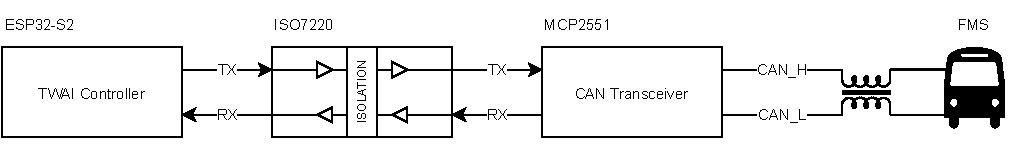
\includegraphics[width=\textwidth]{images/can-interface}
	\vspace{0.0cm}
	\caption{Simplified CAN Interface}
	\label{fig:can-interface}
\end{figure}

\subsubsection{Transceiver}
The data lines are translated using a \acrshort{can} transceiver from Microchip (MCP2551). The role of the transceiver is to drive and detect data to and from the bus. It converts the single-ended logic used by the controller to the differential signal transmitted over the bus. The MCP2551 device provides transmit and receive capabilities and is fully compatible with the \acrshort{iso}-11898 standard.
\newpage

\subsubsection{Isolation}
A dual-channel digital isolator (ISO7221BDR) was used in conjunction with an isolated \acrshort{dc}/\acrshort{dc} converter from Recom (R1SX-3.305/H). These devices block high voltage and isolate grounds, as well as prevent noise currents on a data bus or other circuits from entering the local ground and interfering with or damaging sensitive circuitry.

\begin{figure}[h!]
	\centering
	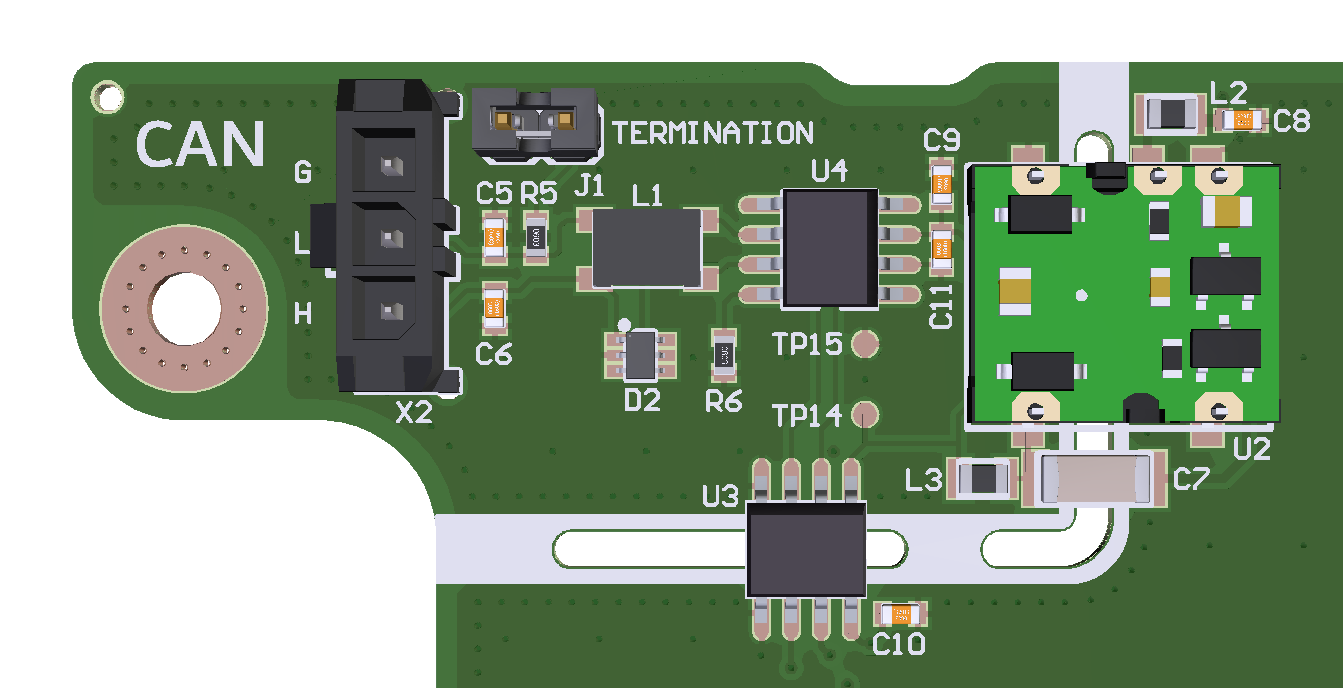
\includegraphics[height=4.5cm]{images/can-pcb}
	\caption{PCB view of CAN interface}
	\label{fig:can-pcb}
\end{figure}

\subsubsection{Filtering}
A common mode choke, as well as bypass capacitors, were added to the differential signal lines. A common mode choke is an electrical filter that blocks high-frequency noise common to two or more data or power lines while allowing the desired \acrshort{dc} or low-frequency signal to pass. \acrfull{cm} noise is typically radiated from sources such as radio signals, unshielded electronics, inverters, and motors. Additionally matching capacitors on the CANH and CANL lines were added to enhance the immunity against electromagnetic interference. 

\subsubsection{Connector}
The \acrshort{fms} Standard specifies a \acrshort{din} 72585 connector as the default physical interface. Since these connectors are only available for panel mount, an additional wire-to-board connector was selected. A Molex Micro-Fit\,3.0 was chosen because it is widely available and being used in lots of applications.

\subsubsection{Termination}
In addition the \acrshort{fms} Standard specifies a 120\,$\Omega$ \acrshort{can} termination resistor to be added on the monitor side. To fulfill this requirement and to make it compatible with systems that do not need that resistor, a jumper was added to enable/disable the termination. 

\subsection{Accelerometer}
By request of the industry partner, an accelerometer was added to gather additional data. The LIS2DH12 is an ultra-low-power high-performance three-axis linear accelerometer with digital \acrshort{i2c}/\acrshort{spi} serial interface output. The sensor has user-selectable scales of ±2\,g up to ±16\,g and is capable of measuring accelerations with data rates from 1\,Hz to 5.3\,kHz. The sensor is connected through \acrshort{spi} to the \gls{esp32}.

\newpage
\section{Mechanical Design}
The automotive environment is known for its harsh conditions, such as vibrations, large temperature fluctuation and high humidity. To ensure long-term reliability, the device must be resistant to these factors. To meet the requirements and achieve an IP67 rating, optimal component selection was critical. Especially the selection of connectors was crucial. 
An enclosure made of polycarbonate with a transparent lid has been selected as a suitable case for the device. The very robust construction creates an ideal protection for all electronic components.\newline
The case has been machined in the internal workshop of the university. The corresponding mechanical drawings have been made with SolidWorks\;2020 and are attached in the Appendix: \ref{Fleet-Monitor V1.0 Mechanical Drawing}

\medskip
\begin{figure}[h!]
	\centering
	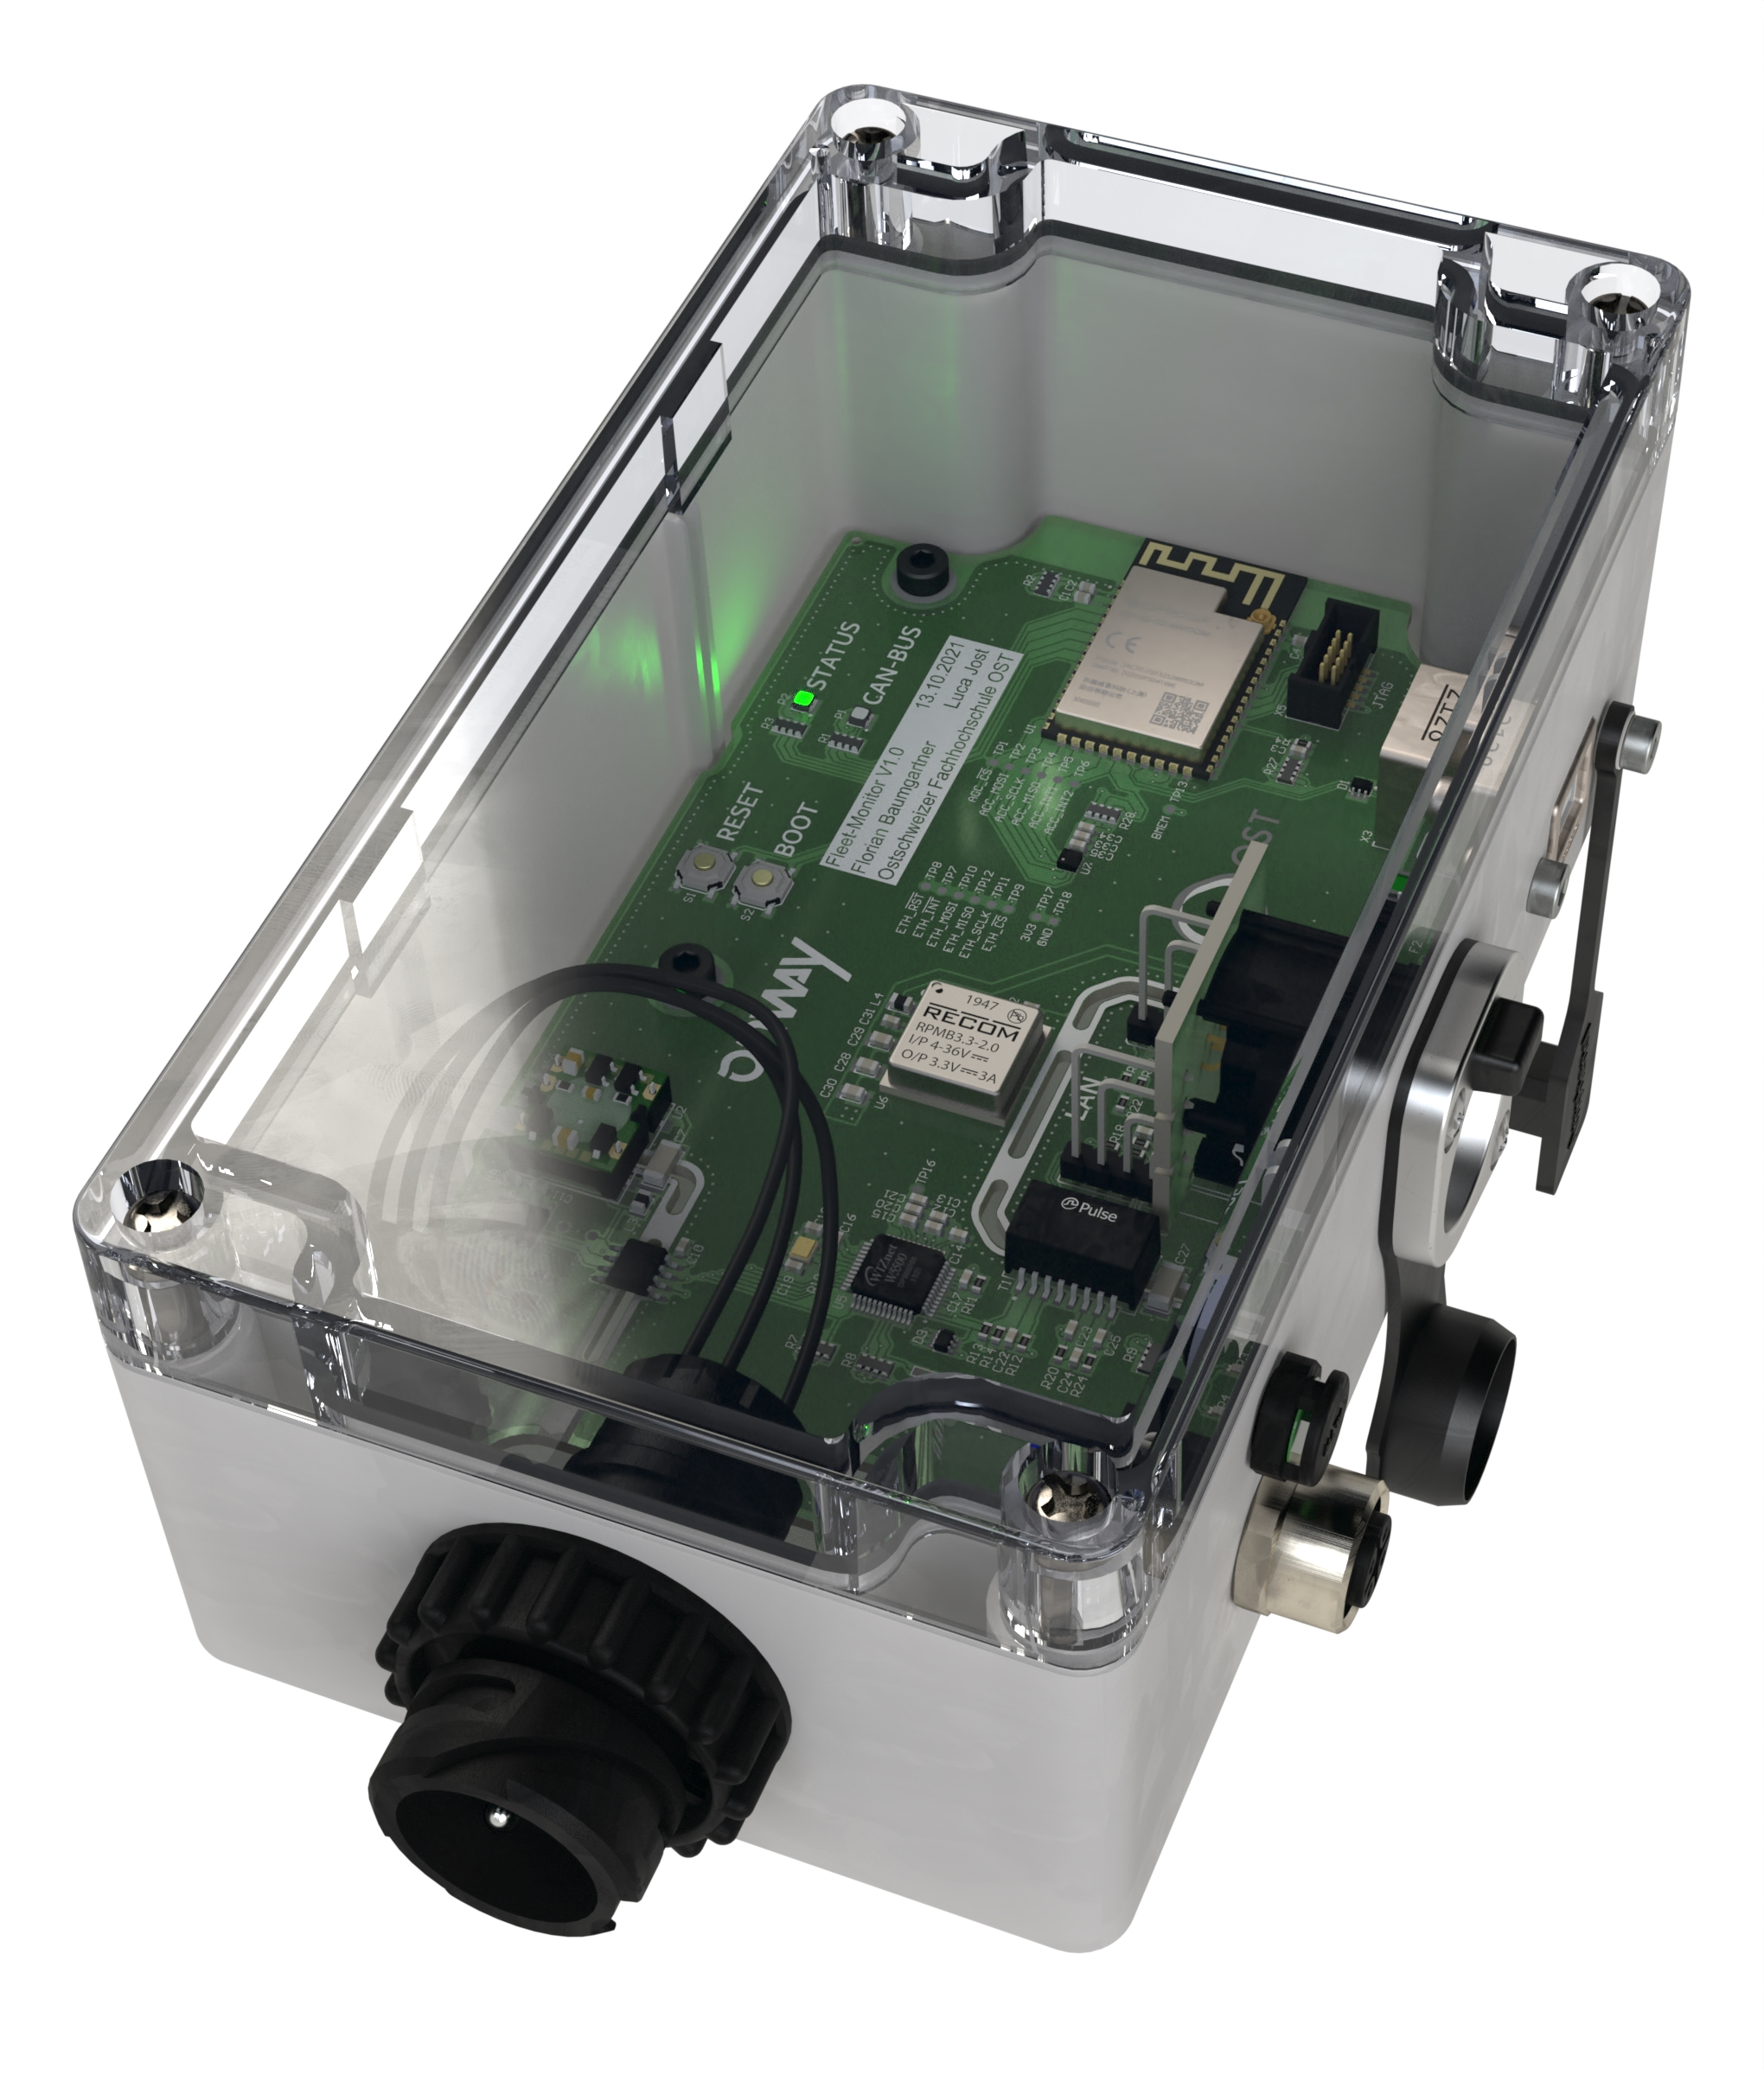
\includegraphics[height=16.5cm]{images/fleet-monitor-rendering}
	\caption{Final Product 3D-Render}
	\label{fig:fleet-monitor-rendering}
\end{figure}
\newpage

%% Section Firmware %%
\section{Firmware}
The firmware is written in C++ and is based on a combination of the \gls{arduino} and the \gls{esp-idf} framework. As an \acrshort{ide}, Visual Studio Code with \gls{platformio} as an add-on has been used. This modern environment ensures rapid and effective development.\newline
FreeRTOS has been used as a real-time operating system, which guarantees a reliable operation and handles multi-task operations on single-core systems.\newline
The Arduino framework offers extensive library support, especially for the \acrshort{usb} peripheral, file system and Ethernet interface. Thousands of users in the \gls{arduino} community make the framework more robust and reliable than other alternatives.

\subsection{File system}
The file system is an essential part of the device firmware. It enables accessing files stored on the internal \acrshort{spi}-Flash chip as well as creating an interface for additional libraries.
The flash chip has a memory capacity of 4\,MB and is partitioned into four different sections. The size of each partition can be configured in the \textit{partitions\_custom.csv} file. The two largest partitions are used for program memory and file system storage. Each of them has ruffly the size of $\approx$ 2\,KB.

\begin{table}[h]
    \begin{tabular}{ | m{3.15cm} | m{3.15cm}| m{3.15cm} | m{3.15cm} |} 
      \hline
      \multicolumn{1}{|c|}{\textbf{Name}} & \multicolumn{1}{c|}{\textbf{Type}} & \multicolumn{1}{c|}{\textbf{Offset}} & \multicolumn{1}{c|}{\textbf{Size}}\\ \hline
      nvs & data & \codeword{0x009000} & 20K \\ \hline
      otadata & data & \codeword{0x00E000} & 8K \\  \hline
      app0 & app & \codeword{0x010000} & 2048K \\  \hline
      ffat & data & \codeword{0x210000} & 1984K \\  \hline
    \end{tabular}
    \caption{\label{tab:Flash-Partitions}SPI-Flash Partitions}
\end{table}

To provide a sufficient set of features, multiple libraries had to be used. Most of them are created by Adafruit Industries under \acrshort{mit} licensing. \newline
As a low-level \acrshort{spi}-Flash chip driver, the \codeword{Adafruit SPIFlash} library has been used. It handles the communication over the physical interface and provides access to the file system library named  \codeword{SdFAT}. The type of file system is \acrshort{fat}, which has the advantage of being compatible with most modern operating systems (Windows/Linux/Mac OS). Figure \ref{fig:file_system_stack} shows an overview of all utilized core libraries and how they are dependent.

\bigskip
\begin{figure}[h!]
	\centering
	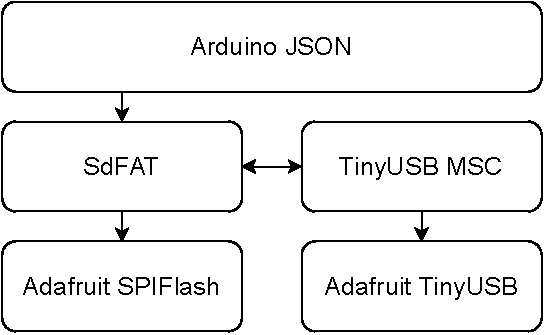
\includegraphics[height=5.2cm]{images/file_system_stack.pdf}
	\caption{USB and File System Library Stack}
	\label{fig:file_system_stack}
\end{figure}
\newpage


\subsection{USB Mass Storage Device}
\acrshort{usb} is known to be a very complex interface, however it provides lots of comfort to an end-user. To enable \acrshort{usb} support on an embedded system, several layers of software are needed. Fortunately, the open source project called TinyUSB supports the \gls{esp32}-S2 \acrshort{soc} family. This very comprehensive software stack supports the \acrshort{usb} \acrfull{msc} protocol.
As a result, the device acts just like a regular \acrshort{usb} Flash drive and provides seamless file access to any host computer. \newline
To pack all setup and configuration functions of the mentioned libraries together, utility functions were made. The \codeword{utils_init()} function checks if the \acrshort{spi}-Flash chip has already been correctly formatted, if this is not the case, an automatic formatting procedure gets executed. In this process, a disk label can be set with a maximal length of 8 characters, in this case: \codeword{MONITOR}. The code section below shows how those utility functions are called at the beginning of the program execution.

\bigskip
\colorlet{mygray}{black!30}
\colorlet{mygreen}{green!60!blue}
\colorlet{mymauve}{red!60!blue}
\begin{lstlisting}[backgroundcolor=\color{gray!10},  
                   basicstyle=\ttfamily,
                   columns=fullflexible,
                   breakatwhitespace=false,      
                   breaklines=true,                
                   captionpos=b,                    
                   commentstyle=\color{mygreen}, 
                   extendedchars=true,              
                   frame=single,                   
                   keepspaces=true,             
                   keywordstyle=\color{blue},      
                   language=c++,                 
                   numbers=none,                
                   numbersep=5pt,                   
                   numberstyle=\tiny\color{blue}, 
                   rulecolor=\color{mygray},        
                   showspaces=false,
                   showstringspaces=false,
                   showtabs=false,                 
                   stepnumber=5,                  
                   stringstyle=\color{mymauve},    
                   tabsize=2,                      
                   title=\lstname,
                   frame=none,
                   xleftmargin = 1cm,
                   framexleftmargin = 1em]
utils_init("MONITOR");  // Initialize peripherals and file system
utils_systemConfig("system.json");   // Load system configuration
utils_startMsc();       // Start USB mass storage controller
\end{lstlisting}

In addition to the \acrshort{usb} \acrshort{msc} protocol, a \acrfull{cdc} has been set up. This creates a \acrfull{vcp} over which the host computer can gain debug information from the device. \newline
After initializing the \acrshort{usb}-Interface and file system, the device configuration is loaded from the locally stored \acrshort{json}-File, more details in the section \ref{System Configuration}.

\subsection{JSON Parser Library} \label{JSON Parser Library}
Due to the frequent usage of the \acrshort{json}-File format in this project, using an advanced software library was key to accelerating the development process. \\
In this case, the open source ArduinoJSON library has been used. It makes use of modern C++14 syntax and is optimized for small architectures like microcontrollers. In addition, support for static and dynamic data allocation simplifies the serializing and deserializing of files without a predefined size. This is especially useful for parsing incoming data over the networking interface. \\[0.5em]
The following code snippet shows how to iterate over a list of elements. If a matching entry has been found, the corresponding name gets returned as a char string. This example shows how the iterating feature can be applied intuitively and how fields can be manipulated dynamically.

\bigskip
\colorlet{mygray}{black!30}
\colorlet{mygreen}{green!60!blue}
\colorlet{mymauve}{red!60!blue}
\begin{lstlisting}[backgroundcolor=\color{gray!10},  
                   basicstyle=\ttfamily,
                   columns=fullflexible,
                   breakatwhitespace=false,      
                   breaklines=true,                
                   captionpos=b,                    
                   commentstyle=\color{mygreen}, 
                   extendedchars=true,              
                   frame=single,                   
                   keepspaces=true,             
                   keywordstyle=\color{blue},      
                   language=c++,                 
                   numbers=none,                
                   numbersep=5pt,                   
                   numberstyle=\tiny\color{blue}, 
                   rulecolor=\color{mygray},        
                   showspaces=false,
                   showstringspaces=false,
                   showtabs=false,                 
                   stepnumber=5,                  
                   stringstyle=\color{mymauve},    
                   tabsize=2,                      
                   title=\lstname,
                   frame=none,
                   xleftmargin = 1cm,
                   framexleftmargin = 1em]
for (JsonVariant value : doc["frames"].as<JsonArray>())
{
  if (strncmp(value["pgn"].as<const char*>(), pgnStr, 4) == 0)
  {
    return value["name"].as<const char*>();
  }
}
\end{lstlisting}


\newpage

\subsection{System Configuration} \label{System Configuration}
The system configuration is defined in a \acrshort{json}-File called \codeword{system.json}, stored in the root directory of the file system. This file is loaded on every startup. The following parameter can be configured:

\begin{table}[h]
    \hfuzz=23.0pt
    \begin{tabular}{ | p{2.8cm} | p{1.3cm} | p{5.9cm} | p{2.7cm} |}
      \hline
      \multicolumn{1}{|c|}{\textbf{Parameter}} & \multicolumn{1}{c|}{\textbf{Type}} & \multicolumn{1}{c|}{\textbf{Description}} & \multicolumn{1}{c|}{\textbf{Example}}\\ \hline
      \codeword{ssid} & string & \acrshort{ssid} of \acrfull{ap} & \codeword{"network"} \hfuzz=3.0pt  \\ \hline
      \codeword{password} & string & Password of \acrshort{ap} * & \codeword{"secret"} \\ \hline
      \codeword{connection} & string & Preferred connection type: \newline\codeword{[auto, lan, wlan]}  & \codeword{"auto"} \\ \hline
      \codeword{config} & string & Location of config file: \newline\codeword{[local, remote]} & \codeword{"remote"} \\ \hline
      \codeword{host_ip} & string & \acrshort{ip} Address of host server & \codeword{"10.3.141.1"} \\ \hline
      \codeword{host_port} & integer & Port of host server & \codeword{8080} \\ \hline \hfuzz=10.0pt 
      \codeword{overwrite_file} & boolean & Overwrite locally stored config file with remotely downloaded version & \codeword{True} \\ \hline
      \codeword{bootloader} & boolean & Restart device in \acrshort{dfu} mode ** & \codeword{False} \\ \hline
    \end{tabular}
    \caption{\label{tab:System-Configuration}System Configuration Parameter Description}
\end{table}

* Password field gets cleared after config file has been loaded due to security reasons.
** If set \codeword{True}, device reboots immediately in \acrshort{dfu} mode and field gets reset to \codeword{False}.

\subsection{Frame Filter Configuration} \label{Frame Filter Configuration}
The configuration of the \acrshort{fms}-Frame filter is based on a specific \acrshort{json}-File called \codeword{config.json}, which is stored in the root directory of the file system. In addition the filter configuration can be downloaded from the host server if the \codeword{config} parameter in the system configuration is set to \codeword{remote}. This allows the user to adjust parameters while the device is in operation, even without physical access.
Basically the \acrshort{json}-File consists of two types of configuration parameters. First of all the general settings which describe how the data should be uploaded to the server: \\[0.3em]
\codeword{framename} enables or disables the transmission of the \acrshort{fms}-Packet name. Turning off this parameter, reduces the overall data upload size and thus minimizes network traffic. For debugging purpose, enabling this setting can help identifying \acrshort{fms}-Frames. \\[0.3em]
\codeword{unknownframes} enables or disables the transmission of unknown \acrshort{fms}-Packets, meaning frames that are not listed in the configuration settings. \\[0.3em]
The second part of the configuration file contains a look-up table with \acrshort{fms}-Frame information and filter settings in form of a list. The different filter types are further described in section \ref{FMS Frame Handler}. Each entry consists of multiple fields specified as followed:

\begin{table}[h!]
    \hfuzz=23.0pt
    \begin{tabular}{ | p{1.4cm} | p{2.2cm} | p{8.9cm} |} \hline
      \multicolumn{1}{|c|}{\textbf{Parameter}} & \multicolumn{1}{c|}{\textbf{Type}} & \multicolumn{1}{c|}{\textbf{Description}} \\ \hline 
      \codeword{pgn} & \acrshort{ascii}-HEX & \acrfull{pgn} as 4 digit number \hfuzz=3.0pt  \\ \hline
      \codeword{name} & string & Human friendly frame name \hfuzz=3.0pt  \\ \hline
      \codeword{active} & boolean & Transmission state, \codeword{False} means ignore frame type \hfuzz=3.0pt  \\ \hline
      \codeword{filter} & string & Filter type: \codeword{[nofilter, change, interval]} \hfuzz=3.0pt  \\ \hline
      \codeword{time} & integer & Max. interval time in [ms], field exists only if filter type is set to \codeword{interval} \hfuzz=3.0pt  \\ \hline
    \end{tabular}
    \caption{\label{tab:frame-parameter-description}Frame Filter Parameter Description}
\end{table}

%\newpage
The following example shows how the \acrshort{json}-File is structured. For better visibility some of the packet settings have been hidden.

\begin{table}[h!]
    \begin{center}
    \framebox{
        \begin{tabular}{p{0.0cm} p{0.1cm} p{0.1cm} p{0.1cm} p{7.0cm}}                                       \\[-0.5em]
        & \multicolumn{4}{l}{$\triangledown$ \texttt{JSON \{3\}}}                                           \\[0.3em]
        & & \multicolumn{3}{l}{\scalebox{0.8}{$\square$} \texttt{framename:\;\ \ \quad\textbf{True}}}       \\[0.3em]
        & & \multicolumn{3}{l}{\scalebox{0.8}{$\square$} \texttt{unknownframes:\;\textbf{False}}}           \\[0.3em]
        & & \multicolumn{3}{l}{$\triangledown$ \texttt{frames [34]}}                                        \\[0.3em]
        & & & \multicolumn{2}{l}{$\triangledown$ \texttt{0 \{4\}}}                                          \\[0.3em]
        & & & & \scalebox{0.8}{$\square$} \texttt{pgn:\;\ \quad\textbf{FEE9}}                               \\[0.3em]
        & & & & \scalebox{0.8}{$\square$} \texttt{name:\;\quad\textbf{Fuel Consumption:\;LFC}}               \\[0.3em]
        & & & & \scalebox{0.8}{$\square$} \texttt{active:\;\textbf{True}}                                   \\[0.3em]
        & & & & \scalebox{0.8}{$\square$} \texttt{filter:\;\textbf{nofilter}}                               \\[0.3em]
        & & & \multicolumn{2}{l}{$\triangledown$ \texttt{1 \{4\}}}                                          \\[0.3em]
        & & & & \scalebox{0.8}{$\square$} \texttt{pgn:\;\ \quad\textbf{FE6C}}                               \\[0.3em]
        & & & & \scalebox{0.8}{$\square$} \texttt{name:\;\quad\textbf{Tachograph:\;TCO1}}                    \\[0.3em]
        & & & & \scalebox{0.8}{$\square$} \texttt{active:\;\textbf{True}}                                   \\[0.3em]
        & & & & \scalebox{0.8}{$\square$} \texttt{filter:\;\textbf{interval}}                               \\[0.3em]
        & & & & \scalebox{0.8}{$\square$} \texttt{time:\;\ \ \textbf{100}}                                  \\[0.3em]
        & & & \multicolumn{2}{l}{$\triangledown$ \texttt{2 \{4\}}}                                          \\[0.3em]
        & & & & \scalebox{0.8}{$\square$} \texttt{pgn:\;\ \quad\textbf{FE4E}}                               \\[0.3em]
        & & & & \scalebox{0.8}{$\square$} \texttt{name:\;\quad\textbf{Door Control 1:\;DC1}}                 \\[0.3em]
        & & & & \scalebox{0.8}{$\square$} \texttt{active:\;\textbf{True}}                                   \\[0.3em]
        & & & & \scalebox{0.8}{$\square$} \texttt{filter:\;\textbf{change}}                                 \\[0.3em]
        & & & \multicolumn{2}{l}{$\triangledown$ \texttt{3 \{4\}}}                                          \\[0.3em]
        & & & & \scalebox{0.8}{$\square$} \texttt{pgn:\;\ \quad\textbf{FDA5}}                               \\[0.3em]
        & & & & \scalebox{0.8}{$\square$} \texttt{name:\;\quad\textbf{Door Control 2:\;DC2}}                 \\[0.3em]
        & & & & \scalebox{0.8}{$\square$} \texttt{active:\;\textbf{False}}                                  \\[0.3em]
        & & & & \scalebox{0.8}{$\square$} \texttt{filter:\;\textbf{nofilter}}                               \\[0.3em]
        & & & \multicolumn{2}{l}{$\triangledown$ \texttt{4 \{4\}}}                                          \\[0.3em]
        & & & & \scalebox{0.8}{$\square$} \texttt{pgn:\;\ \quad\textbf{FEEA}}                               \\[0.3em]
        & & & & \scalebox{0.8}{$\square$} \texttt{name:\;\quad\textbf{Vehicle Weight:\;VW}}                  \\[0.3em]
        & & & & \scalebox{0.8}{$\square$} \texttt{active:\;\textbf{True}}                                   \\[0.3em]
        & & & & \scalebox{0.8}{$\square$} \texttt{filter:\;\textbf{interval}}                               \\[0.3em]
        & & & & \scalebox{0.8}{$\square$} \texttt{time:\;\ \ \textbf{5000}}                                 \\[0.3em]
        & & & \multicolumn{2}{l}{$\rhd$ \texttt{5 \{4\}}}                                                   \\[0.3em]
        & & & \multicolumn{2}{l}{$\rhd$ \texttt{6 \{4\}}}                                                   \\[0.3em]
        & & & \multicolumn{2}{l}{...}                                                                       \\[0.3em]
        & & & \multicolumn{2}{l}{$\rhd$ \texttt{34 \{4\}}}                                                  \\[0.4em]
        \end{tabular}
    }
    \end{center}
\vspace{-0.3cm}
\caption{\label{fig:frame-configuration-example}Frame Filter Configuration Example}
\end{table}
\newpage

\subsection{Networking}  \label{Networking}
The Fleet-Monitor needs to communicate with a server to stream data, exchange the current time and read configuration data. 
\subsubsection{Connection}
The device can connect through WiFi or Ethernet with the host. Both interfaces utilize \acrshort{dhcp} to negotiate an \acrshort{ip} address and the server \acrshort{ip} can be configured through the system configuration. The device can be connected to both interfaces at the same time but only one is used to communicate with the server. 

The connection is checked every 5\,seconds and works as follows. First the hardware status is checked, then the connection to a host and lastly if we received an \acrshort{ip} address. The Ethernet interface is the prioritized communication method. It provides better data throughput and is less prone to errors than the over the air alternative. For example, if both interfaces received an \acrshort{ip} address and are able to communicate with the server, Ethernet is used for the transmission. This is illustrated in Figure \ref{fig:connectin-tree} bellow.
\begin{figure}[!ht]
	\centering
	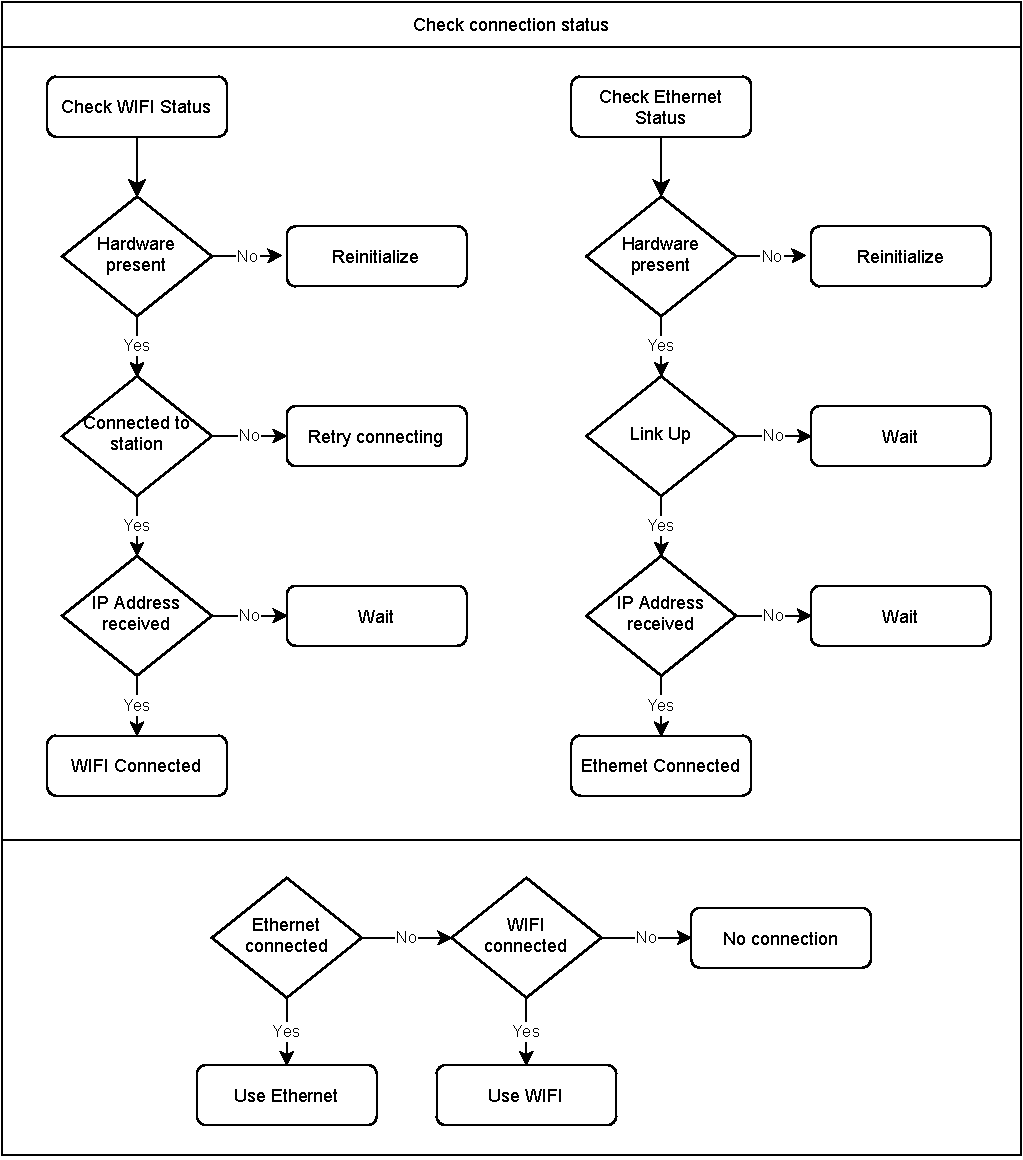
\includegraphics[height=14.5cm]{images/connection-tree}
	\caption{Flow chart of interface selection}
	\label{fig:connectin-tree}
\end{figure}
\newpage

\subsubsection{HTTP}
\acrfull{http} is used to communicate with the server and allows the Fleet-Monitor to read files and stream data. We decided to go with this technology because it is well supported by all libraries used. Data is transferred using \acrshort{http} POST requests containing data inside the body. The server response is used to check if the data was received correctly and validate the server connection. \acrshort{http} GET methods are used to read files from the server.

\subsubsection{Time synchronization}
In order for data to be useful it needs to have a timestamp. Ideally this timestamp would translate to a real time and date. This is why we implemented on both the server and client side a mechanism to synchronize the two. Every POST response from the server includes a \acrshort{json} string with a field called Date. This field represents the current date and time and is used by the Fleet-Monitor to set its real time clock. Since the \gls{esp32}-S2 WROOM module does not have a dedicated oscillator for time keeping, the default 40\,MHz crystal is used. This oscillator has a tolerance of ±\,10\,\acrshort{ppm}. The maximum 24\,hour drift can be calculated using the Equation \ref{eq:time}.
\medskip
\begin{equation}
\delta_{rel} =  \frac{1}{f} * \frac{f * \mathit{p}}{10^6} * t = \frac{1}{40\,MHz} * \frac{40\,MHz * \pm\,10}{10^6} * 86400\,s =  \pm\,0.864\,s  
\label{eq:time}
\end{equation}

where:

\begin{conditions}
 f     &  frequency in Hz \\
 \mathit{p}     &  deviation in \acrshort{ppm} \\
 t     &  time in s \\
\end{conditions}

Since this drift is quite large, we decided to update the real time clock of the \gls{esp32}-S2 every 24\,h to make sure both the server and the Fleet-Monitor always share the same time.

The timestamp is read out as \codeword{YYYY,MM,DD,hh,mm,ss} format and is stored locally in \gls{unix} time. 

\subsubsection{File Reload}
Additionally a mechanism was developed to automatically detect if a configuration file needs to be reloaded. A reload is needed when the file on the server was modified. Every \acrshort{http} POST response contains a \acrshort{json} field called \texttt{ConfigReload}. If this flag is set we will request the configuration file again from the server in order to clear the flag and get the newest configuration. The local configuration can be overwritten with the one from the server, if the option is selected in the system configuration.

\newpage
\subsection{FMS Frames} \label{FMS Frame Handler}
Reading out frames from the \acrshort{can} bus, filtering them and finally transmitting them to the server is done using two FreeRTOS tasks and a FreeRTOS queue. Figure \ref{fig:fms-software} illustrates this task view. The frame handler task has the highest priority as task switching while transmitting can cause issues.
\begin{figure}[h!]
	\centering
	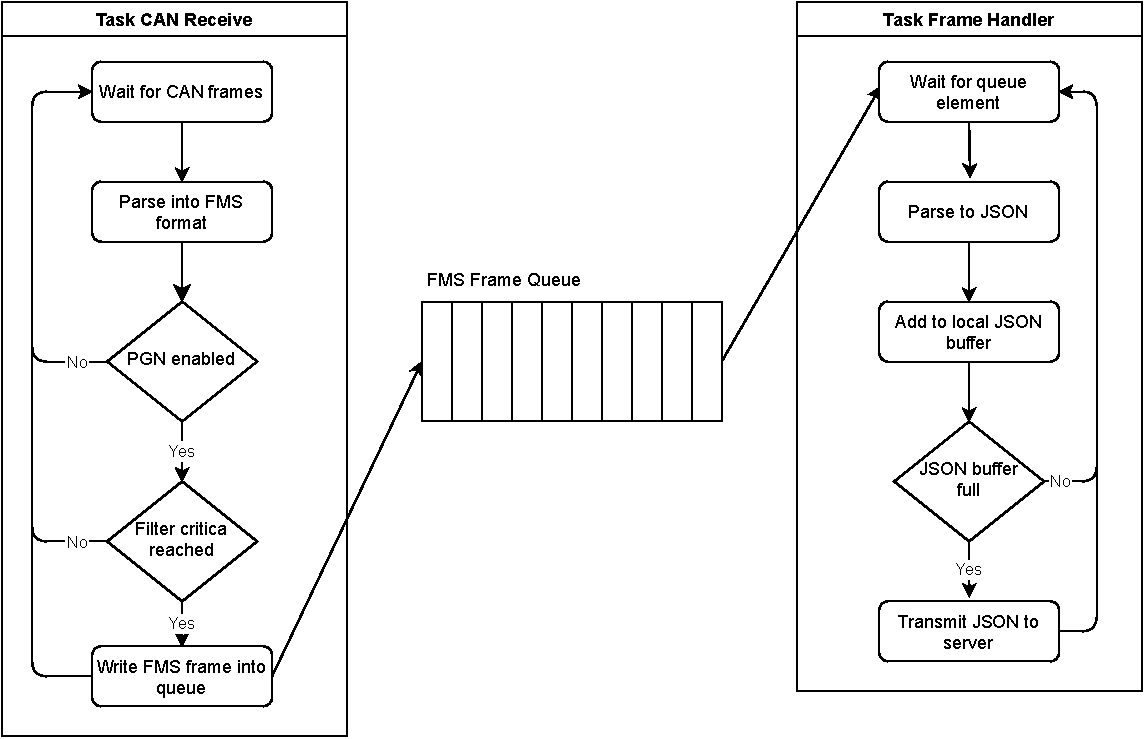
\includegraphics[width=\textwidth]{images/fms-software}
	\caption{FreeRTOS Tasks and Queue for FMS Frames}
	\label{fig:fms-software}
\end{figure}

\subsubsection{FMS Filter}
Both tasks will only begin its execution once a configuration was read from either the server or from the local file system. The configuration is explained in the Section \ref{Frame Filter Configuration}.

Generally a frame can be enabled and disabled for the transmission, this helps remove unwanted packages from taking up valuable bandwidth. Additionally three filter methods were implemented to reduce the data rate and repetition of useless information:
\begin{itemize}
		\item \textit{On Change}, data is only transmitted when something inside the data field of the frame has changed. This is very useful for state supervision of error codes or door states. 
		\item \textit{Interval}, data is only transmitted with a set interval. Data in between the set interval is discarded. This filter method is used for things that are not very important but still good to know from time to time.
		\item \textit{No Filter}, all the data received is being transmitted. This method is used for things that need real-time supervision.
\end{itemize}

Data inside the queue is always sent out to the server. Therefore the filtering is done inside the \acrshort{can}-Read task and only adds data to the queue when it passes all the filters.  

\subsubsection{JSON Format}
In order to hold the \acrshort{fms} data from the queue, a \acrshort{json} buffer is allocated. The timestamp is added to each frame, and then all the other fields are added to the \acrshort{json} array. The user can enable and disable the name in the configuration file. Adding the name simplifies parsing, but increases the data rate since it is added to every frame.

\begin{table}[h!]
    \begin{center}
    \framebox{
        \begin{tabular}{p{0.0cm} p{0.1cm} p{0.1cm} p{0.1cm} p{7.0cm}}                                       \\[-0.5em]
        & \multicolumn{4}{l}{$\triangledown$ \texttt{JSON \{1\}}}                                           \\[0.3em]
        & & \multicolumn{3}{l}{$\triangledown$ \texttt{frames [n]}}                                         \\[0.3em]
        & & & \multicolumn{2}{l}{$\triangledown$ \texttt{0 \{4\}}}                                          \\[0.3em]
        & & & & \scalebox{0.8}{$\square$} \texttt{ts:\;\ \ \textbf{1618892400.420}}                         \\[0.3em]
        & & & & \scalebox{0.8}{$\square$} \texttt{pgn:\;\ \textbf{FEE9}}                                    \\[0.3em]
        & & & & \scalebox{0.8}{$\square$} \texttt{data:\;\textbf{FFFFFFFF000236A4}}                         \\[0.3em]
        & & & & \scalebox{0.8}{$\square$} \texttt{name:\;\textbf{Fuel Consumption:\;LFC}}                    \\[0.3em]
        & & & \multicolumn{2}{l}{$\triangledown$ \texttt{1 \{4\}}}                                          \\[0.3em]
        & & & & \scalebox{0.8}{$\square$} \texttt{ts:\;\ \ \textbf{1618892400.690}}                         \\[0.3em]
        & & & & \scalebox{0.8}{$\square$} \texttt{pgn:\;\ \textbf{FE6C}}                                    \\[0.3em]
        & & & & \scalebox{0.8}{$\square$} \texttt{data:\;\textbf{ACF1E302FFFF00F7}}                         \\[0.3em]
        & & & & \scalebox{0.8}{$\square$} \texttt{name:\;\textbf{Tachograph:\;TCO1}}                         \\[0.3em]
        & & & \multicolumn{2}{l}{$\triangleright$ \texttt{2 \{4\}}}                                         \\[0.3em]
        & & & \multicolumn{2}{l}{$\triangleright$ \texttt{3 \{4\}}}                                         \\[0.3em]
        & & & \multicolumn{2}{l}{...}                                                                       \\[0.3em]
        & & & \multicolumn{2}{l}{$\rhd$ \texttt{n \{4\}}}                                                   \\[0.4em]
        \end{tabular}
    }
    \end{center}
\caption{\label{fig:example-fms-data}Example FMS Data for Transmission}
\end{table}

The \acrshort{json} buffer can hold a maximum of 8\,KB. Single frames are added to the buffer until it is filled up. At that point it is ready for the transmission.  

\subsubsection{Transmission}
Data is communicated over the currently active networking interface, as previously explained in Section \ref{Networking}. The \acrshort{json} buffer is serialized into a single string before being sent to the server as part of an \acrshort{http} POST request. In normal operation, the server confirms the request with a status code of \texttt{200}. The \acrshort{json} buffer is discarded if a request to the server times out or if no confirmation is returned. This is due to the large amount of data collected by the bus. The length of the transmission body varies, however it is usually around 8000\,bytes. The period between POST requests is significantly depending on the filter technique, but without any active filters, a transmission occurs around every second.
\newpage

\subsection{Accelerometer}
The acceleration is read out from its own task with an update rate of 50\,Hz. Since we are not using the data at this moment, we just read it out and leave its specific implementation open for the future.

On boot up over a period of 5\,seconds, the accelerometer is calibrated to eliminate the offset on each axis and get rid of the gravity vector. The purpose of this is to make it easy to record high acceleration events. When the linear acceleration reaches a predefined threshold, the data can be transmitted to the server.

The axes of the accelerometer are oriented as shown in Figure \ref{fig:accel-axis}.

\begin{figure}[h!]
	\centering
	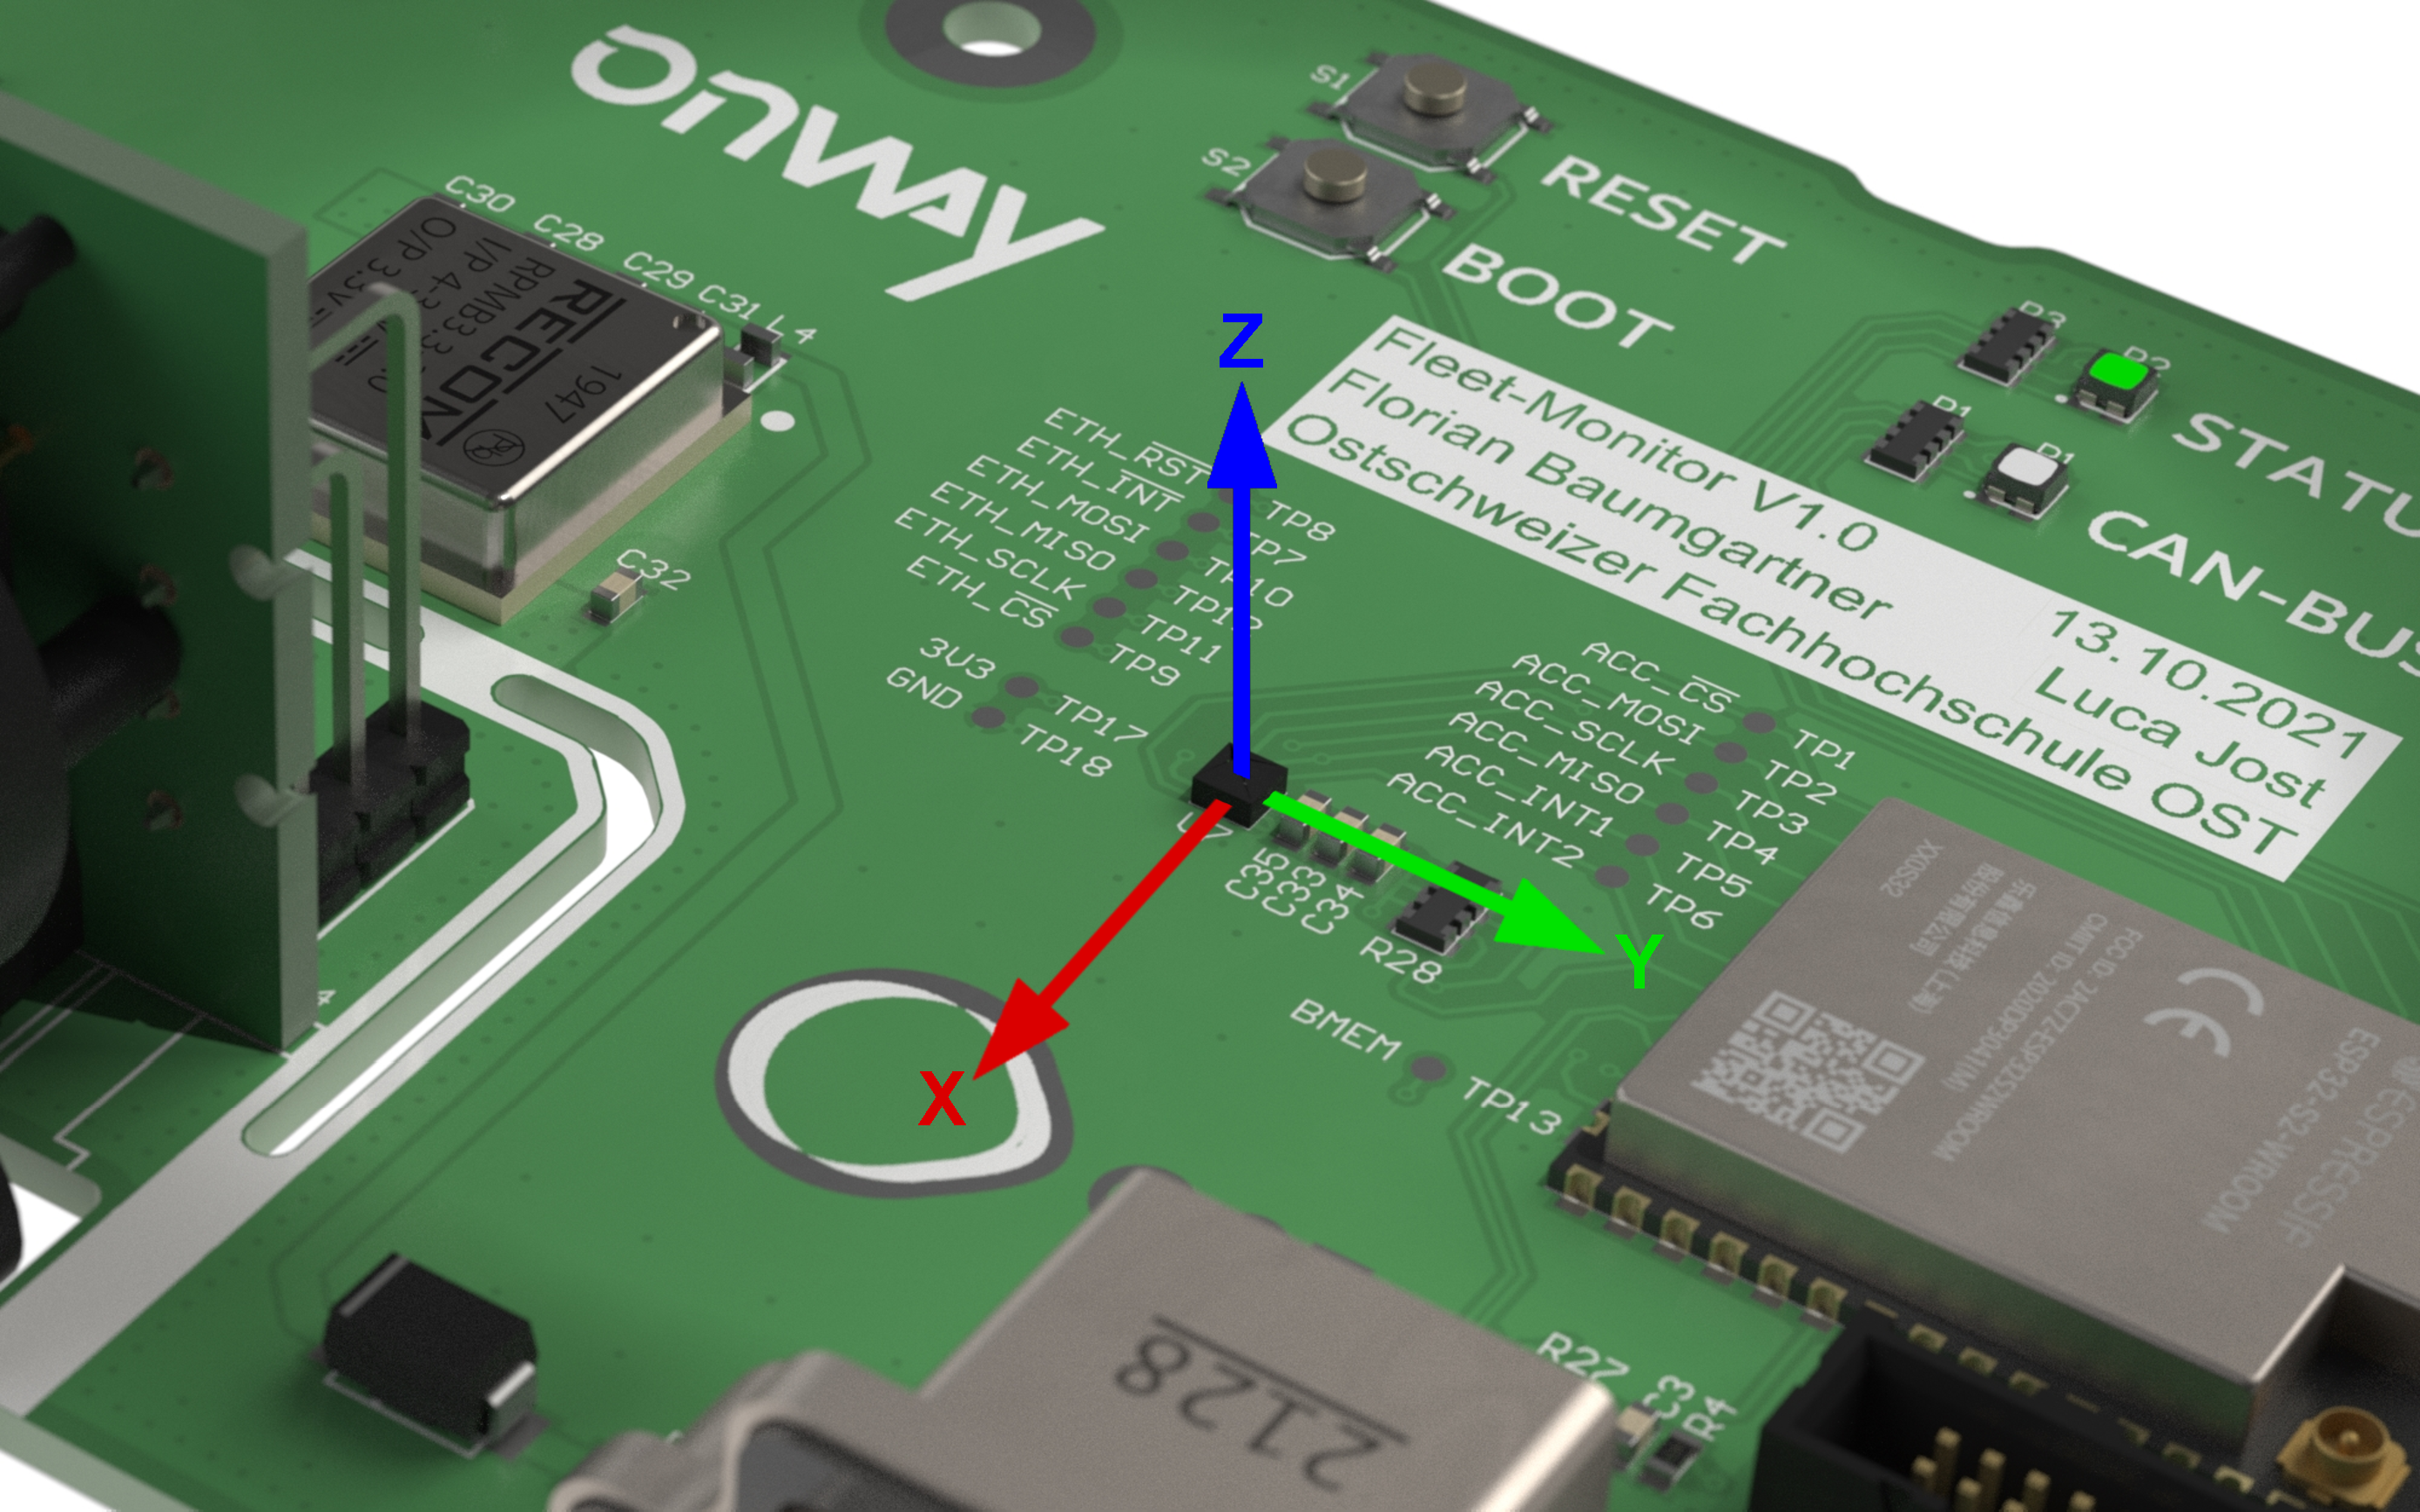
\includegraphics[width=\textwidth]{images/Accel-axis}
	%\vspace{0.0cm}
	\caption{Accelerometer Axes Orientation}
	\label{fig:accel-axis}
\end{figure}

\newpage
\section{Utility Software Tools}
Several software tools have been developed to support the hardware in its operation and to simplify the configuration of the device. These utilities were all written in the Python programming language. As a suitable platform to run the applications, a Raspberry Pi 400 was selected for its price and performance.

\subsection{HTTP Server}
A \acrshort{http} server was developed to communicate with the Fleet-Monitor. It was written with the help of an \acrshort{ai} system that translates natural language to code called \gls{openai-codex}. It helped us to reduce the development time and produced comprehensive results for our application. The \acrshort{http} Server is a command line application that does not have a graphical user interface. Both \acrshort{http} GET and \acrshort{http} POST requests can be handled by the server. Each request to the server creates a new thread that will handle the response. Making it possible to handle multiple requests at the same time.

\acrshort{http} GET requests are used to access files stored locally. Filenames are included in the \acrshort{url} of the \acrshort{http} GET request. Using this method, multiple files may be served. If the requested file is located in the servers directory, the server responds with status code \texttt{200} and serves it. Otherwise, an empty page is returned with a status code of \texttt{404}.

Streaming data from the Fleet-Monitor to the server is extremely important for our application. To accomplish this we are using \acrshort{http} POST requests. The server expects a \acrshort{json} string of \acrshort{fms} data inside the body of the request, if the data is found and no errors are detected it will respond with a status code of \texttt{200}. Moreover, the server will include the current time and date in the response, along with the information if a file has been changed in its directory. The \acrshort{json} string from the request is split and then stored locally in a \acrshort{csv} file. By using the \acrshort{fms} Data Visualizer, the data can then be interpreted. Example \acrshort{csv} data:

\bigskip
\colorlet{mygray}{black!30}
\colorlet{mygreen}{green!60!blue}
\colorlet{mymauve}{red!60!blue}
\begin{lstlisting}[backgroundcolor=\color{gray!10},  
                   basicstyle=\ttfamily,
                   columns=fullflexible,
                   breakatwhitespace=false,      
                   breaklines=true,                
                   captionpos=b,                    
                   commentstyle=\color{mygreen}, 
                   extendedchars=true,              
                   frame=single,                   
                   keepspaces=true,             
                   keywordstyle=\color{blue},      
                   language=Python,                 
                   numbers=none,                
                   numbersep=5pt,                   
                   numberstyle=\color{blue}, 
                   rulecolor=\color{mygray},        
                   showspaces=false,
                   showstringspaces=false,
                   showtabs=false,                 
                   stepnumber=5,                  
                   stringstyle=\color{mymauve},    
                   tabsize=2,                      
                   title=\lstname,
                   frame=none,
                   xleftmargin = 1cm,
                   framexleftmargin = 1em]
0, 1639753080.803,F003,FFD9FFFFFFFFFFFF
1, 1639753080.814,FE6C,485352203C330000
2, 1639753080.846,F004,FFFFFF8039FFFFFF
3, 1639753080.857,F003,FFD9FFFFFFFFFFFF
4, 1639753080.868,FE6C,5768792061726520 
5, 1639753080.911,FE6C,796F75206465636F 
6, 1639753080.921,FE6C,64696E6720746869
7, 1639753080.954,FE6C,733F210000000000
8, 1639753080.964,F003,FFD9FFFFFFFFFFFF
9, 1639753080.975,FE6C,4F53545355434B53
10, 1639753081.18,F003,FFD9FFFFFFFFFFFF
11, 1639753081.29,F004,FFFFFF8039FFFFFF
...

\end{lstlisting}

Both the \acrshort{http} server and a utility tool called \textit{RaspAP} are running on a Raspberry\;Pi. \textit{RaspAP} is used to create an \acrlong{ap} and configures the networking ports to act as a router, making it possible to connect to it over WiFi and Ethernet.
\newpage

\newpage
\subsection{FMS Configuration Tool}
Changing the configuration of the \acrshort{fms}-Frame filter in a text editor is not very pleasant. Therefore a \acrfull{gui} has been developed to make this procedure easier and ensure a better overview of all settings. This tool is able to generate the \acrshort{json}-File structure as mentioned in Section \ref{Frame Filter Configuration}.

\subsubsection{Feature Description}
The configuration tool is divided into \textit{Global Settings} and \textit{Frame Settings}. The general options can be enabled or disabled by clicking on the corresponding checkbox. Further in the Frame Settings section, a table allows the user to change the filter behaviour of each \acrshort{fms}-Packet type. The filter features are described as followed:

\begin{description}
  \item[Active:] Enables or disables the transmission of this specific packet type
  \item[PGN:] Shows the \acrlong{pgn} in hexadecimal format \textit{(Read-Only)}
  \item[Name:] Shows the user friendly packet name \textit{(Read-Only)}
  \item[Filter:] Combo-box to select the filter type: \textit{No Filter}, \textit{On Change}, \textit{Max. Interval}
  \item[{Interval [ms]:}] Max. update rate, only available if filter type is set to: \textit{Max. Interval}
\end{description}

\medskip
\begin{figure}[h!]
	\centering
	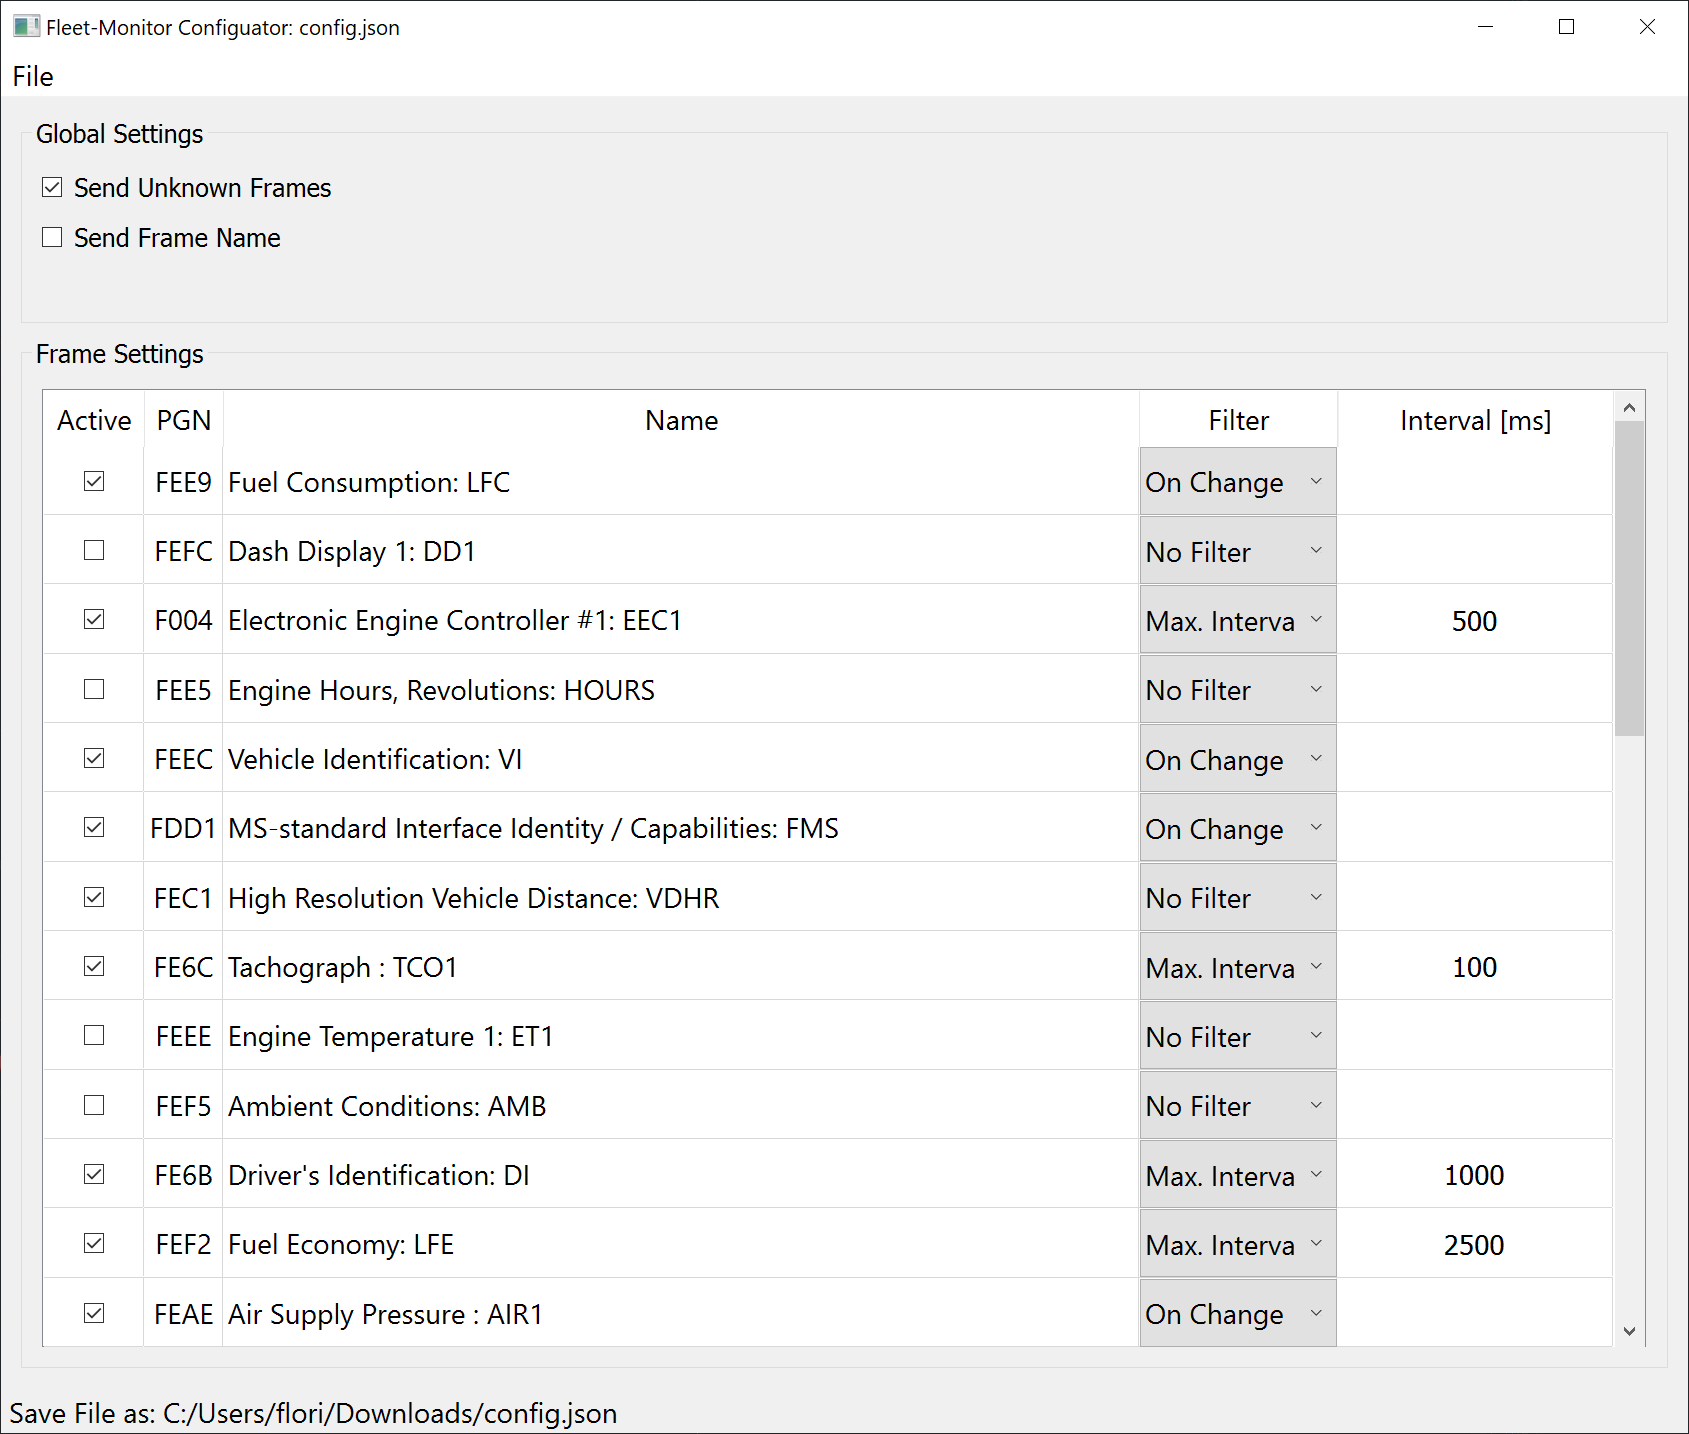
\includegraphics[width=\textwidth]{images/Configuration-Tool_Screenshot}
	\caption{FMS Frame Configuration Tool}
	\label{fig:configuration_tool}
\end{figure}
\newpage

\subsubsection{PyQt5}
As a framework Qt Version 5 for Python, in short PyQt5, was used. This very comprehensive software package enables rapid development of \acrshort{gui}s. One of several major advantages is the platform compatibility. Therefore the tools run on all major operating systems without any changes to the code. The python interpreter executes the code in a closed environment and does only depend on the PyQt5 framework. No additional packages or frameworks are needed. \\
The dynamic scaling of the window including all of its features is essential. Modern applications must be able to run on a variety of screen resolutions.

\subsubsection{File Loading \& Saving}
\begin{wrapfigure}{r}{4.0cm}
\vspace{-0.6cm}
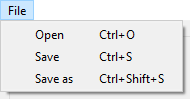
\includegraphics[width=4.0cm]{images/configuration-tool-file-panel}
\caption{File Menu-Bar}
\end{wrapfigure} 
To open an existing configuration file, three methods are available. Firstly via the menu-bar section, by clicking on the \textit{Open} button. Secondly by using the keyboard shortcut \textit{Ctrl+O} and lastly by dragging a file into the application. Saving files is very similar and intuitive due to the use of common shortcuts.
%\newpage

\subsection{FMS Data Visualizer}
Since the host server receives the data in raw HEX format, post processing is needed to gain access to the contained information. To demonstrate this procedure, a Python script has been developed to parse and visualize \acrshort{fms}-Data. 

\subsubsection{FMS Frame Parsing}
The \acrshort{fms}-Standard describes in detail how each frame type can be decoded. In the scope of this project, the focus has been set on parsing the most common frame types. As mentioned in Section\;\ref{Fleet Management System (FMS)}, a frame contains 8\,bytes of data. Figure\;\ref{fig:fms_frame_example} shows an example of how the ambient air temperature is encoded. In this case, only 2\,bytes (Data Byte 4 \& 5) are used. 

\begin{figure}[h!]
	\centering
	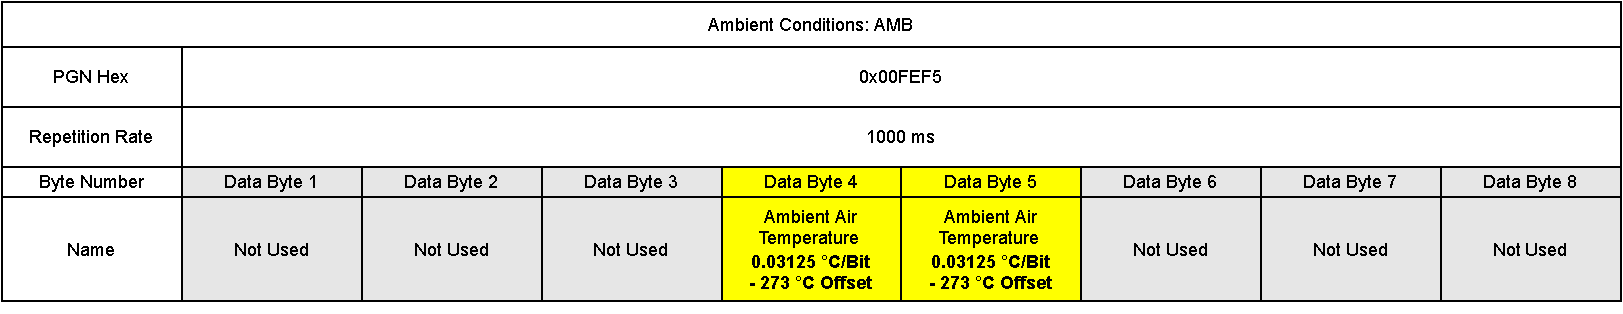
\includegraphics[width=\textwidth]{images/fms_frame_example}
	\caption{FMS Frame Example: Ambient Conditions: AMB \cite{fms-standard-description}}
	\label{fig:fms_frame_example}
\end{figure}

The Python code snippet below shows how to extract the ambient air temperature of the raw input data. The bytes are ordered as \textit{little-endian}. The parser concatenates the individual bytes and applies global scaling and offset. In this case a scaling of 0.03125\,°C\,/\,Bit and an offset of -273\,°C gets applied.

\bigskip
\colorlet{mygray}{black!30}
\colorlet{mygreen}{green!60!blue}
\colorlet{mymauve}{red!60!blue}
\begin{lstlisting}[backgroundcolor=\color{gray!10},  
                   basicstyle=\ttfamily,
                   columns=fullflexible,
                   breakatwhitespace=false,      
                   breaklines=true,                
                   captionpos=b,                    
                   commentstyle=\color{mygreen}, 
                   extendedchars=true,              
                   frame=single,                   
                   keepspaces=true,             
                   keywordstyle=\color{blue},      
                   language=Python,                 
                   numbers=none,                
                   numbersep=5pt,                   
                   numberstyle=\color{blue}, 
                   rulecolor=\color{mygray},        
                   showspaces=false,
                   showstringspaces=false,
                   showtabs=false,                 
                   stepnumber=5,                  
                   stringstyle=\color{mymauve},    
                   tabsize=2,                      
                   title=\lstname,
                   frame=none,
                   xleftmargin = 1cm,
                   framexleftmargin = 1em]
amb = df[df["pgn"] == 0xFEF5]  # Filter data-set by frame type
amb["ambientAir"] = (amb["3"] + amb["4"] * 256) * 0.03125 - 273.0
\end{lstlisting}
\newpage

\subsubsection{List of Supported Frames}
The current version of the \acrshort{fms} Data Visualizer supports parsing the following frame types listed in Table \ref{tab:supported-fms-frames}. Note that this tool is made for demonstration purposes only.

\begin{table}[h!]
    \hfuzz=23.0pt
    \begin{tabular}{ | p{1.4cm} | p{12.2cm} |} \hline
      \multicolumn{1}{|c|}{\textbf{PGN}} & \multicolumn{1}{c|}{\textbf{Frame Name}}     \\ \hline 
      \centering\codeword{FE6C} & Tachograph: TCO1                                      \hfuzz=3.0pt  \\ \hline
      \centering\codeword{FD09} & High Resolution Fuel Consumption (Liquid): HRLFC      \hfuzz=3.0pt  \\ \hline
      \centering\codeword{FEF2} & Fuel Economy: LFE                                     \hfuzz=3.0pt  \\ \hline
      \centering\codeword{FDA5} & Door Control 2: DC2                                   \hfuzz=3.0pt  \\ \hline
      \centering\codeword{FE58} & Air Suspension Control 4: ASC4                        \hfuzz=3.0pt  \\ \hline
      \centering\codeword{FEEE} & Engine Temperature 1: ET1                             \hfuzz=3.0pt  \\ \hline
      \centering\codeword{FE56} & Aftertreatment 1 Diesel Exhaust Fluid Tank 1 Information: AT1T1I \hfuzz=3.0pt  \\ \hline
      \centering\codeword{FEF5} & Ambient Conditions: AMB                               \hfuzz=3.0pt  \\ \hline
      \centering\codeword{FED5} & Alternator Speed: AS                                  \hfuzz=3.0pt  \\ \hline
      \centering\codeword{FEC1} & High Resolution Vehicle Distance: VDHR                \hfuzz=3.0pt  \\ \hline
      \centering\codeword{FEAE} & Air Supply Pressure: AIR1                             \hfuzz=3.0pt  \\ \hline
      \centering\codeword{FEF1} & Cruise Control / Vehicle Speed 1: CCVS1               \hfuzz=3.0pt  \\ \hline
      \centering\codeword{F004} & Electronic Engine Controller \#1: EEC1                \hfuzz=3.0pt  \\ \hline
      \centering\codeword{F003} & Electronic Engine Controller \#2: EEC2                \hfuzz=3.0pt  \\ \hline
    \end{tabular}
    \caption{\label{tab:supported-fms-frames}Supported \acrshort{fms}-Frames by the Python Data-Parser}
\end{table}

\subsubsection{Plotly Library}
As a visualizing framework \textit{Plotly} was used. The framework enables creating modern looking interactive diagrams. A great advantage is the web-based interface which allows updating the plot in real time. The Figure shows an example of visualizing a \acrshort{fms}-Data dump from a public transport bus in Germany.

\begin{figure}[h!]
	\centering
	\hfuzz=15.0pt
	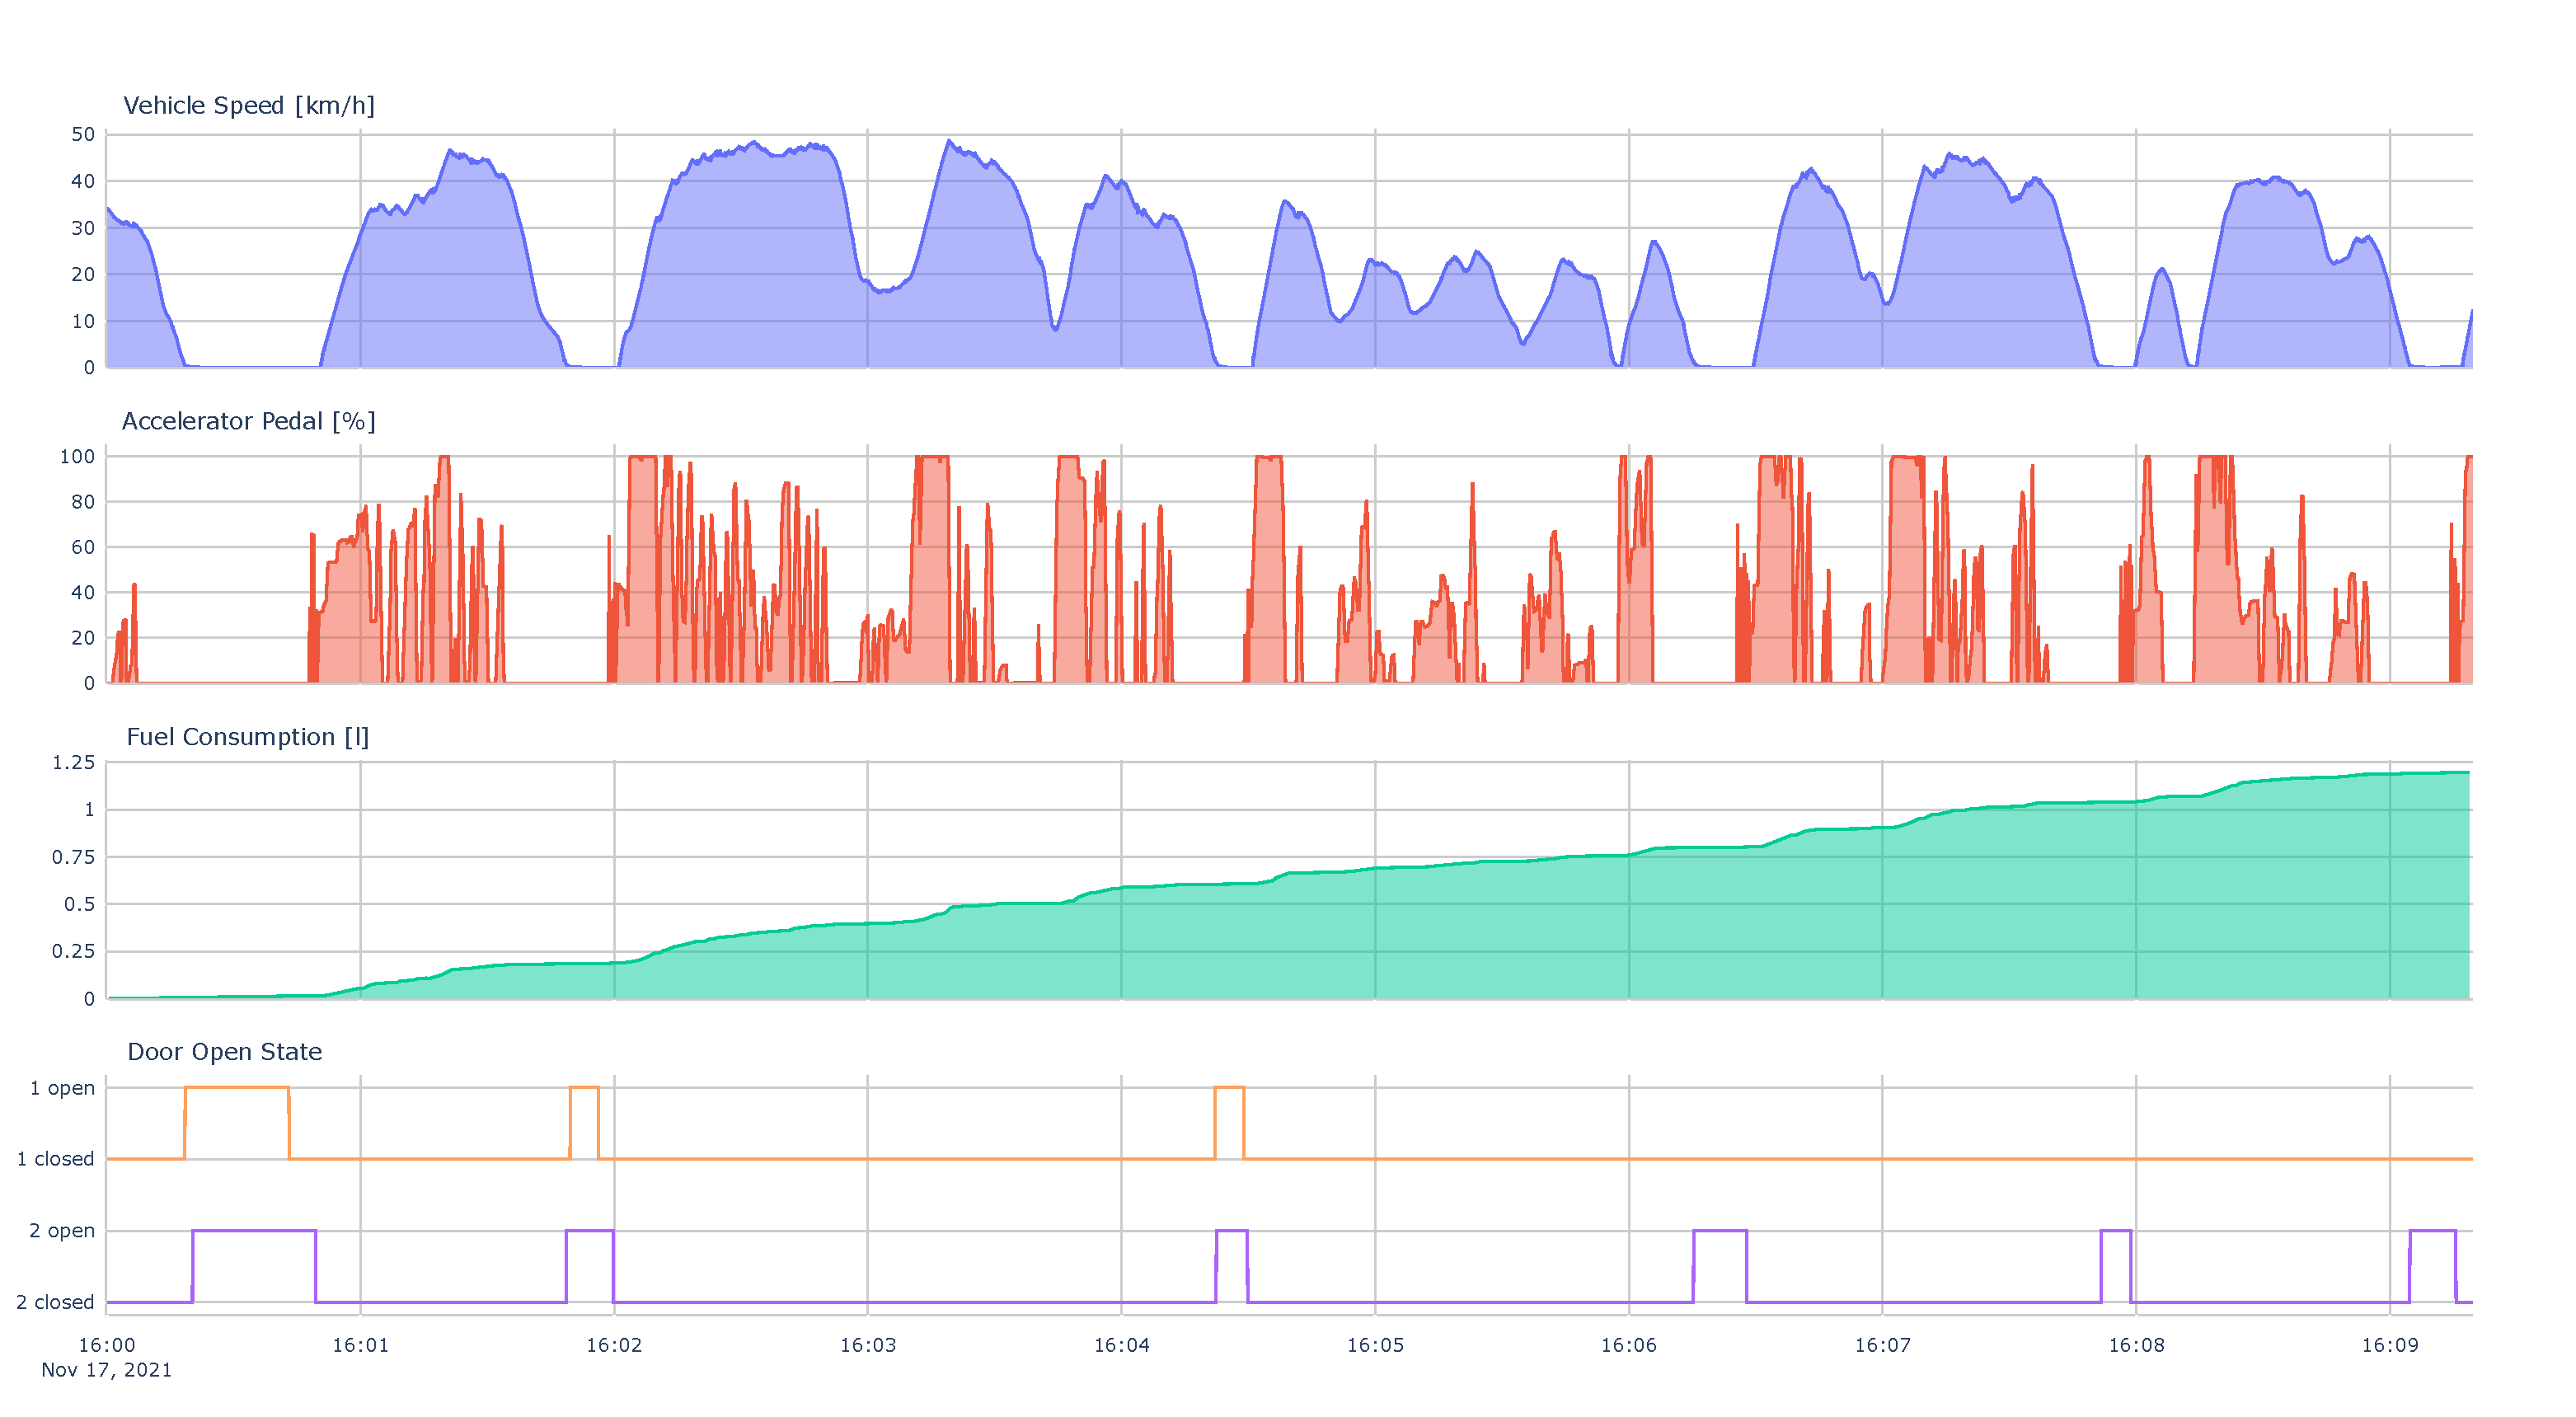
\includegraphics[width=\textwidth]{images/FMS_Data_Visualization.pdf}
	\caption{Visualization of FMS Data}
	\label{fig:fms_visualization}
\end{figure}
\newpage

\addtocontents{toc}{\protect\newpage}   % Start on new page in table of contents 
\chapter{User Manual}
This chapter describes the function and operation of the device, the system specifications and possible error scenarios with a potential cause of the problem. In addition, instructions are available for setting up the device and change the configuration.

\section{Configuration}
\subsection{System Setup}
After production, the blank \gls{esp32}-S2 must be programmed with the latest firmware. This can be achieved by following the steps in Section \ref{Firmware Update}. Next, the system configuration as well as the \acrshort{fms}-frame filter configuration must be loaded onto the root directory of the mass storage device. Figure\;\ref{fig:fleet-monitor-root-directory} shows how the file structure should look like when plugged in to a \acrshort{pc} via the \acrshort{usb}-interface.

\medskip
\begin{figure}[h!]
	\centering
	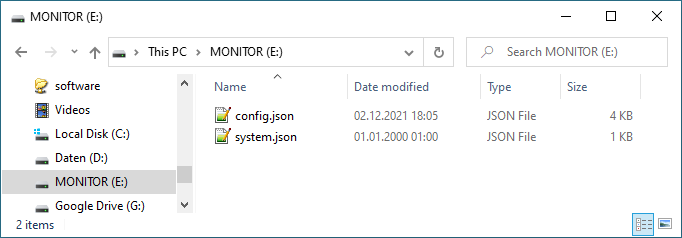
\includegraphics[width=13cm]{images/File_Explorer}
	\caption{Fleet-Monitor Root Directory}
	\label{fig:fleet-monitor-root-directory}
\end{figure}

Furthermore, parameters in the system configuration file must be adjusted to the needs of the overall setup. This contains setting the host \acrshort{ip} address and port number, as well as the \acrshort{ssid} and password if the device should connect over WiFi. Additional options can be defined, please refer to Section \ref{System Configuration} for more information.
\newpage

\subsection{Firmware Update} \label{Firmware Update}
\begin{wrapfigure}{r}{5.2cm}
\vspace{-0.6cm}
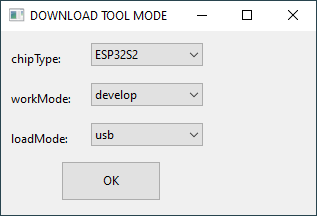
\includegraphics[width=5.2cm]{images/ESP32_Download_Mode}
\vspace{-0.4cm}
\caption{ESP32 Download Tool}
\label{fig:esp32-download-tool}
\end{wrapfigure} 
Espressif offers a firmware download tool for the \gls{esp32}-Family \cite{flash-download-tools}. When starting the application, the options in the dialog box should be set as shown in Figure \ref{fig:esp32-download-tool}. After pressing OK, the main window appears. 
To establish a connection to the \gls{esp32}-S2 over the \acrshort{usb}-interface, it has to be set into \acrshort{dfu}-Mode. This can be achieved by pressing the \textit{boot} button while resetting or power-cycling the device. If the device is already programmed with a firmware version that supports entering the \acrshort{dfu} mode by software, the \texttt{bootloader} flag can be set to \texttt{true} in the system configuration file as mentioned in Section \ref{System Configuration}.

The next step is to load the binary files at a specific location (offset as HEX index) in the flash memory. The first three files are called \texttt{bootloader\_qio\_40m.bin}, \texttt{partitions.bin} and \texttt{boot\_app0.bin}. These files are independent of the firmware and must not be changed. The fourth file called \texttt{firmware.bin} can be loaded directly from the build folder of the \acrshort{ide} (e.g. Visual Studio Code) and placed at offset \codeword{0x10000}. \\
In this case the following path is used: \texttt{FleetMonitor$\backslash$.pio$\backslash$build$\backslash$esp32s2dev}

Change the programming options of the download tool so that they exactly match Figure\;\ref{fig:esp32s2-download-tool-settings}. Now select the correct COM-Port and press the \texttt{START} button. It takes around 10\;seconds to upload the firmware. After updating, the device has to be reset and the new firmware gets executed. Note that this procedure does not touch the file system and therefore no data is being lost.

\begin{figure}[h!]
	\centering
	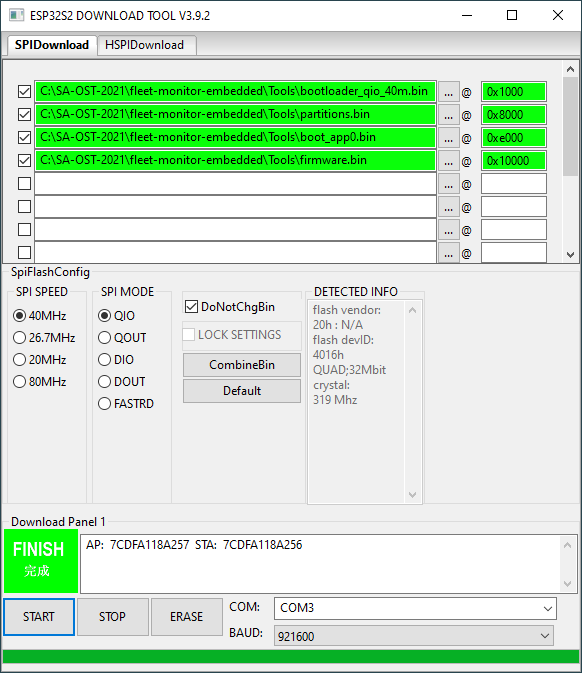
\includegraphics[width=9.2cm]{images/ESP32_Firmware_Settings}
	\caption{ESP32S2 Download Tool Settings}
	\label{fig:esp32s2-download-tool-settings}
\end{figure}
\newpage

\section{Specifications}
\begin{center}
    \begin{tabular}{p{6.4cm} p{6.4cm}}
    %\hline
    External Input Voltage          & 9\,V - 28\,V                      \\ %\hline
    Power Consumption               & 2.5\,W                            \\ %\hline
    Dimensions (L x W x D)          & 160 x 89 x 61\,mm                 \\ %\hline
    Weight                          & 350\,g                            \\ %\hline
    Water Resistance Rating         & IP67                              \\ %\hline
    Power Connector                 & M12 R/A F                         \\ %\hline
    Microprocessor                  & ESP32-S2                          \\ %\hline
    LAN-Interface                   & 10\,Base-T / 100\,Base-TX         \\ %\hline
    WLAN-Interface                  & 802,11b/g/n                       \\ %\hline
    USB-Interface                   & USB 2.0 (Device)                  \\ %\hline
    CAN-Interface                   & 250\,kbit/s (SAE J1939)           \\ %\hline
    
    \end{tabular}
\end{center}

\section{Device Status and Troubleshooting}


\subsection{LED Status}
The Fleet-Monitor uses two \acrshort{rgb} \acrshort{led}s to indicate the current status. Additionally there are two \acrshort{led}s located to the left of the RJ45 connector showing the link status and link activity.

\begin{center}
    \begin{tabular}{| p{6.4cm} | p{6.4cm} |} \hline
    \multicolumn{1}{|c|}{\textbf{Status LED}} & \multicolumn{1}{c|}{\textbf{Description}}   \\ \hline 
    White breathing                 & System is booting up                                  \\ \hline
    Blue breathing                  & System tries to connect to network                    \\ \hline
    Green                           & Connected to server over Ethernet                     \\ \hline
    Yellow                          & Connected to server over WiFi                         \\ \hline
    Magenta                         & Unable to establish server connection                 \\ \hline
    Red blinking                    & Unable to load configuration file                     \\ \hline
    
    \end{tabular}
\end{center}

\begin{center}
    \begin{tabular}{| p{6.4cm} | p{6.4cm} |} \hline
    \multicolumn{1}{|c|}{\textbf{CAN LED}} & \multicolumn{1}{c|}{\textbf{Description}}      \\ \hline 
    Off                             & Device is not receiving \acrshort{can} data           \\ \hline
    Green blinking                  & Device is receiving \acrshort{can} data               \\ \hline
    Red blinking                    & Error on physical interface                           \\ \hline
    \end{tabular}
\end{center}
\newpage

\subsection{Resolving Issues} \label{Resolving Issues}

\subsubsection{Status LED breathing white}
Normally this status clears within one or two breathing cycles. If the status does not clear the device is most likely in a boot loop. If this happens something is seriously wrong with the hard- or software. Refer to Section \ref{Hard Reset} for a resolution.

\subsubsection{Unable to connect to network}
The blue \acrshort{led} will breathe while the device is trying to establish a network connection. Connecting over WiFi or Ethernet can take up to one minute. The status is cleared as soon as a connection is received and an \acrshort{ip} address was assigned. If no connection can be established over an extended period of time the following things should be checked in order.

\textbf{Connecting over WiFi:}
\begin{enumerate}
  \item Make sure the device is not obstructed and close to the \acrlong{ap} in order to establish a connection. Metals, carbon fiber, and other \acrshort{rf} shielding materials should be kept away from the antenna of the \gls{esp32}.
  \item Make sure the \acrlong{ap} is password protected with \acrshort{wpa} or \acrshort{wpa}2. Both \acrshort{wep} and \acrshort{wpa}3 are not supported.
  \item Make sure the \acrlong{ap} name and password are set correctly in the system configuration. Please limit your passwords to \acrshort{ascii} characters, special Unicode characters are not allowed. Remember, the system automatically clears the password from the \texttt{system.json} file after a reboot but stores it locally.
  \item Make sure other devices like phones or computers can reach the \acrlong{ap}. If they are unable to, you may have a problem on the \acrshort{ap} side.
\end{enumerate}

\textbf{Connecting over Ethernet:}
\begin{enumerate}
  \item Make sure the \acrshort{led}s on the left side of the RJ45 connector are showing activity. If that is not the case check the following things.
  \begin{itemize}
      \item Make sure the \acrlong{ap} is powered on.
      \item Make sure the RJ45 cable is plugged in completely on both sides.
      \item Make sure the RJ45 cable is not faulty.
      \item Try connecting another device to the RJ45 cable and see if it receives a connection.
  \end{itemize}
  If all of these checks pass you may have a soft- or hardware issue. Refer to Section \ref{Hard Reset} for a resolution.
  \item Make sure the \acrlong{ap} is capable of \acrshort{dhcp}. The Fleet-Monitor gets the \acrshort{ip} address through the \acrlong{dhcp}. There is no support for static \acrshort{ip} addresses.
\end{enumerate}
\newpage

\subsubsection{Unable to establish server connection}\label{Unable to establish server connection}
If the status \acrshort{led} is not cleared after a short while, the Fleet-Monitor is unable to establish a connection to the server. The device is connected to an \acrshort{ap}, received an \acrshort{ip} address but the \acrshort{http} POST requests are unanswered or a bad status is returned. The following things should be checked to resolve this issue.

\begin{enumerate}
  \item Make sure the \acrshort{http} server is running and can respond to POST requests. The Fleet-Monitor is expecting to receive a response from the server with the status code of \texttt{200}. Otherwise, it will not clear the error.
  \item Make sure the \acrshort{ip} address and port are configured correctly in the system configuration file.
  \item Make sure to check if a request times out or an error code is returned from the server. The Fleet-Monitor will print the server response to the serial port. Section \ref{Serial Monitor} explains how to access the serial port.
\end{enumerate}

\subsubsection{Unable to load configuration file}
If the status \acrshort{led} is blinking red the device was unable to load the configuration file. 

A missing or corrupt file system is possible if the configuration can not be loaded locally.

To force manual reformatting of the file system, the \textit{boot} button must be pressed for 5 seconds while the device is in operation (not during a reset of the device).\\
\textbf{ATTENTION: THIS PROCEDURE WILL DELETE ALL FILES!}

In case the system is configured to load the file from the server you may need to refer to the error: Unable to establish server connection \ref{Unable to establish server connection}. The only difference is that these requests are done with \acrshort{http} GET instead of POST. Make sure your server can handle the requests to the Fleet-Monitor's specification.

\subsubsection{Device is not receiving CAN data}
In case the \acrshort{can} \acrshort{led} is turned off, the device is unable to receive data from the \acrshort{can} bus. You may want to try the following things.

\begin{enumerate}
  \item Make sure the \acrshort{can} termination is enabled on both ends of the bus.
  \item Make sure the \acrshort{can} data polarity is correct (CANH / CANL).
  \item Make sure the cable has the correct pin-out and no wires are damaged. 
  \item Make sure the \acrshort{fms} Gateway from the vehicle is transmitting data.
\end{enumerate}

\subsubsection{CAN Hardware Error}
In case the \acrshort{can} \acrshort{led} is blinking red, something went wrong in the initialization process of the \acrshort{can} interface. You may need to do a hard reset explained in Section \ref{Hard Reset}.

\newpage

\subsection{Serial Monitor} \label{Serial Monitor}
Diagnostics information is printed to the serial monitor to help the user debug an issue. Accessing the terminal can be done in just a few steps.

\begin{enumerate}
  \item Get a serial terminal tool for your computer. If you are running Windows, \mbox{\textit{TeraTerm}} is highly recommended. 
  \item Connect the Fleet-Monitor to your computer with a \acrshort{usb} cable.
  \item Locate the assigned serial port (e.g. using the \textit{Device Manager} on Windows).
  \item Run your serial terminal tool and connect to the open port. In \mbox{\textit{TeraTerm}}, under \textit{File {$\rightarrow$} New Connection} the serial port can be selected as shown in Figure \ref{fig:tera-connect}. Your port may vary. 
  \begin{figure}[h!]
	\centering
	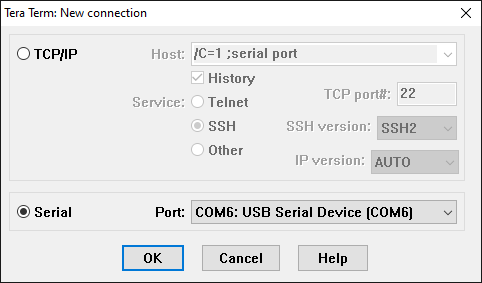
\includegraphics[width=9.2cm]{images/tera-connect}
	\caption{Open serial port through \mbox{\textit{TeraTerm}}}
	\label{fig:tera-connect}
\end{figure}
    \item Information is now being printed to the terminal and should look something like the example below.
    \bigskip
    \colorlet{mygray}{black!30}
    \colorlet{mygreen}{green!60!blue}
    \colorlet{mymauve}{red!60!blue}
    \begin{lstlisting}[backgroundcolor=\color{gray!10},  
                       basicstyle=\ttfamily,
                       columns=fullflexible,
                       breakatwhitespace=false,      
                       breaklines=true,                
                       captionpos=b,                    
                       commentstyle=\color{mygreen}, 
                       extendedchars=true,              
                       frame=single,                   
                       numbers=none,                
                       numbersep=5pt,                   
                       numberstyle=\color{blue}, 
                       rulecolor=\color{mygray},        
                       showspaces=false,
                       showstringspaces=false,
                       showtabs=false,                 
                       stepnumber=5,                  
                       stringstyle=\color{mymauve},    
                       tabsize=2,                      
                       title=\lstname,
                       frame=none,
                       xleftmargin = 1cm,
                       framexleftmargin = 1em]
    Connected over WiFi
    Loading config from server
    Status code: 200
    Config loading successful!
    \end{lstlisting}
\end{enumerate}

\subsection{Hard Reset} \label{Hard Reset}
If there is a serious issue with the device, the first action should be to reformat the file system and then upload the configuration files again. If this did not resolve the problem you may want to flash a known to be working firmware to the device. This is explained in Section \ref{Firmware Update}. If the issue persists, some parts of the hardware could be damaged and need to be replaced.

\chapter{Summary \& Conclusion}
To summarize, a fully comprehensive device has been developed. With it, additional software tools were created to support the hardware in its operation and to simplify the configuration for the user. The \acrshort{fms}-Monitor enables onway customers to get access to low-level vehicle data in a very convenient manner. In order to prove the functionality, five reliable and production-ready prototypes have been produced. The devices were tested over an extended period of time with a J1939 simulator. A test report was written and can be found in the Appendix \ref{Test Reports}.

All requirements defined in the task definition have been satisfied. The only pending aspect is the transmission of accelerometer data. The implementation of this feature has been neglected, due to the insufficiently detailed description of the operation. However, this functionality can easily be added in the future if necessary.

\section{Continuing Work}
Although the designed prototypes provide a rich set of features, there are some aspects to improve or features to add.  Of particular note is the fact that the system is designed for future enhancements. As an example, the flash storage of the \gls{esp32}-S2 provides lots of additional storage for larger firmware editions.\\
The following continuations are possible:

\begin{itemize}
		\item Testing the device in the field (e.g. installed in a bus). The test results can show the impact of harsh weather conditions, vibrations and other environmental influences. 
		\item Adding \acrfull{ota} firmware update support to the device. This feature could provide quick bug-fixes and simplifying the addition of custom features. It would accelerate the updating process especially for larger fleets.
		\item Porting the Python based \acrshort{http} server application to dedicated onway hardware (network router).
		\item Cost reduction of the hardware. This can be achieved by different assembly options (e.g. with/without physical Ethernet interface).
		\item Implementation of accelerometer data transmission.
\end{itemize}

\newpage
\section{Reflection \& Project Schedule}
Our time management was excellent, all milestones were reached as scheduled and all functions were implemented on time. There were some parts of the firmware that turned out to be more complicated than expected, resulting in long workdays in order to stay on schedule. It proved to be a very substantial decision, to switch from the \gls{esp-idf} framework to \gls{arduino} based core libraries. This has helped drastically to get the \acrshort{usb}-Interface and file system working. The \gls{esp-idf} lacks software support in these areas. Further, assembly and testing of the hardware took almost three times longer than we originally planned. This was caused by a small oversight in the schematic of the device, which led to a bad connection. After having rectified the problem in the Ethernet controller circuitry, everything else went smoothly.

\section{Personal Reflections}

\subsubsection{Florian Baumgartner}
This student research project allowed me to get involved to the \acrshort{can} interface and the \acrshort{fms} protocol. Further I could make use of my previously gained knowledge in the field of embedded systems and software engineering. It was a very positive experience to develop a fully working product in such a small time frame. The detailed planing of the project proved to be very important. Thus, I'm especially proud of meeting each milestone on time and preventing major delays. \newline
It was a pleasure to work with Luca Jost and we had overall a great time working on this project. My personal highlight was learning the PyQt5 framework as well as using the Plotly library. I'm fairly interested in the field of \acrshort{iot} devices, therefore this project was a great opportunity to deepen my knowledge and getting more experienced.

I'm glad that the hardware development went that smoothly although the ongoing worldwide chip shortage made it difficult to get access to the components needed. It payed out to premature focus on this particularly challenging situation and chose parts that were easily available. All in all, good communication was key to lead to a successful result.

\subsubsection{Luca Jost}
In general, this student research project overall has been very enjoyable. Within just a few weeks, we transformed an idea into a deployment-ready product. The Fleet-Monitor is working as designed and I am looking forward to seeing the device being used in the field. During the project, I was able to leverage my previous experience and build on it. I found it particularly fascinating to learn more about \acrshort{can} systems, as it is a very popular technology in the industry currently. Working with embedded systems is something I have always liked and this project was no exception. Developing real-time operating systems with complex logic is something I enjoy. This project was not particularly complex, and unfortunately, there was nothing that challenged me significantly.

In past projects, I had trouble with time management, so we made sure to develop a realistic timetable this time. Spending the extra time on the schedule has proven to be very advantageous as I was able to deliver all tasks on time. 

The experience of working with Florian Baumgarnter was extremely rewarding; his dedication and attention to detail are admirable.

\appendix
\chapter{Appendix}
\clearpage

\section{Declaration of Authorship} \label{Declaration of Authorship}
We hereby certify that the thesis we are submitting is entirely our own original work except where otherwise indicated. We are aware of the University’s regulations concerning plagiarism, including those regulations concerning disciplinary actions that may result from plagiarism. Any use of the works of any other author, in any form, is properly acknowledged at their point of use.

\bigskip
\textbf{Location, Date} \\
Rapperswil, 03. June 2022

\vspace{1.2cm}
\begin{tabular}{@{}p{0.1cm}p{6cm}p{0.6cm}p{6cm}@{}}
& \hrulefill & & \hrulefill\\ \\[-0.7em]
& Florian Baumgartner & & Thierry Schwaller\\
\end{tabular}


\includegraphics[width=4.8cm, align=t, smash=br, hshift=0.9cm, vshift=2.55cm]{appendix/Signature_Florian_Baumgartner.pdf}
%
\includegraphics[width=4.8cm, align=t, smash=br, hshift=8.25cm, vshift=2.77cm]{appendix/Signature_Thierry_Schwaller.pdf}
\newpage

\iffalse

\section{Fleet-Monitor V1.0 Schematics} \label{Fleet-Monitor V1.0 Schematics}
\enlargethispage{2.5cm}
\begin{adjustwidth}{-0.23cm}{0cm} \hfuzz=7.0pt \vfuzz=20.0pt
\makebox[\textwidth]{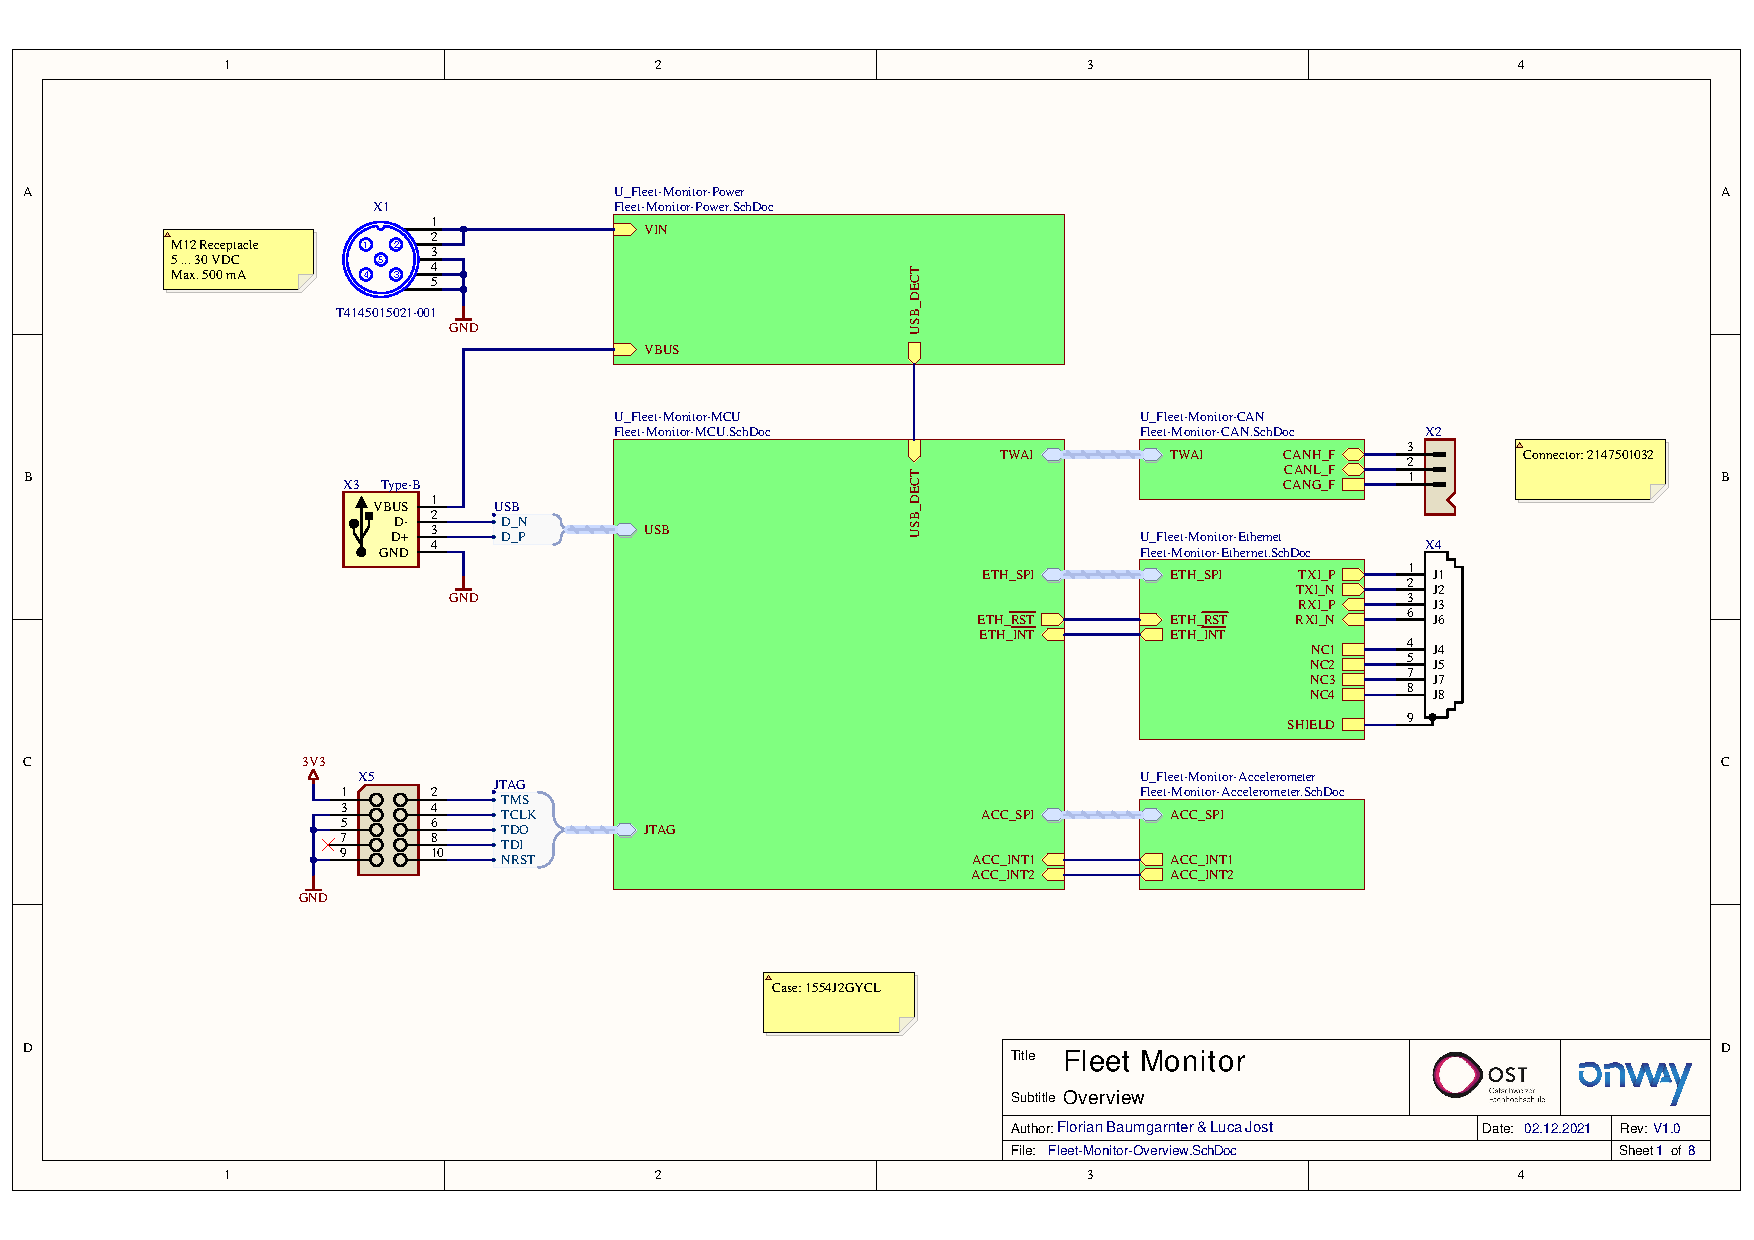
\includegraphics[angle=90, width=17.3cm, page=1]{appendix/Fleet-Monitor Schematics}}
\end{adjustwidth}
\newpage

\begin{adjustwidth}{0.23cm}{0cm} \hfuzz=7.0pt \vfuzz=20.0pt
\makebox[\textwidth]{\includegraphics[angle=90, width=17.3cm, page=2]{appendix/Fleet-Monitor Schematics}}
\end{adjustwidth}
\newpage

\begin{adjustwidth}{-0.23cm}{0cm} \hfuzz=7.0pt \vfuzz=20.0pt
\makebox[\textwidth]{\includegraphics[angle=90, width=17.3cm, page=3]{appendix/Fleet-Monitor Schematics}}
\end{adjustwidth}
\newpage

\begin{adjustwidth}{0.23cm}{0cm} \hfuzz=7.0pt \vfuzz=20.0pt
\makebox[\textwidth]{\includegraphics[angle=90, width=17.3cm, page=4]{appendix/Fleet-Monitor Schematics}}
\end{adjustwidth}
\newpage

\begin{adjustwidth}{-0.23cm}{0cm} \hfuzz=7.0pt \vfuzz=20.0pt
\makebox[\textwidth]{\includegraphics[angle=90, width=17.3cm, page=5]{appendix/Fleet-Monitor Schematics}}
\end{adjustwidth}
\newpage

\begin{adjustwidth}{0.23cm}{0cm} \hfuzz=7.0pt \vfuzz=20.0pt
\makebox[\textwidth]{\includegraphics[angle=90, width=17.3cm, page=6]{appendix/Fleet-Monitor Schematics}}
\end{adjustwidth}
\newpage

\begin{adjustwidth}{-0.23cm}{0cm} \hfuzz=7.0pt \vfuzz=20.0pt
\makebox[\textwidth]{\includegraphics[angle=90, width=17.3cm, page=7]{appendix/Fleet-Monitor Schematics}}
\end{adjustwidth}
\newpage

\begin{adjustwidth}{0.23cm}{0cm} \hfuzz=7.0pt \vfuzz=20.0pt
\makebox[\textwidth]{\includegraphics[angle=90, width=17.3cm, page=8]{appendix/Fleet-Monitor Schematics}}
\end{adjustwidth}
\newpage


\section{Fleet-Monitor V1.0 BOM} \label{Fleet-Monitor V1.0 BOM}
\enlargethispage{1.6cm}
\begin{adjustwidth}{-0.23cm}{0cm} \hfuzz=7.0pt \vfuzz=20.0pt
\makebox[\textwidth]{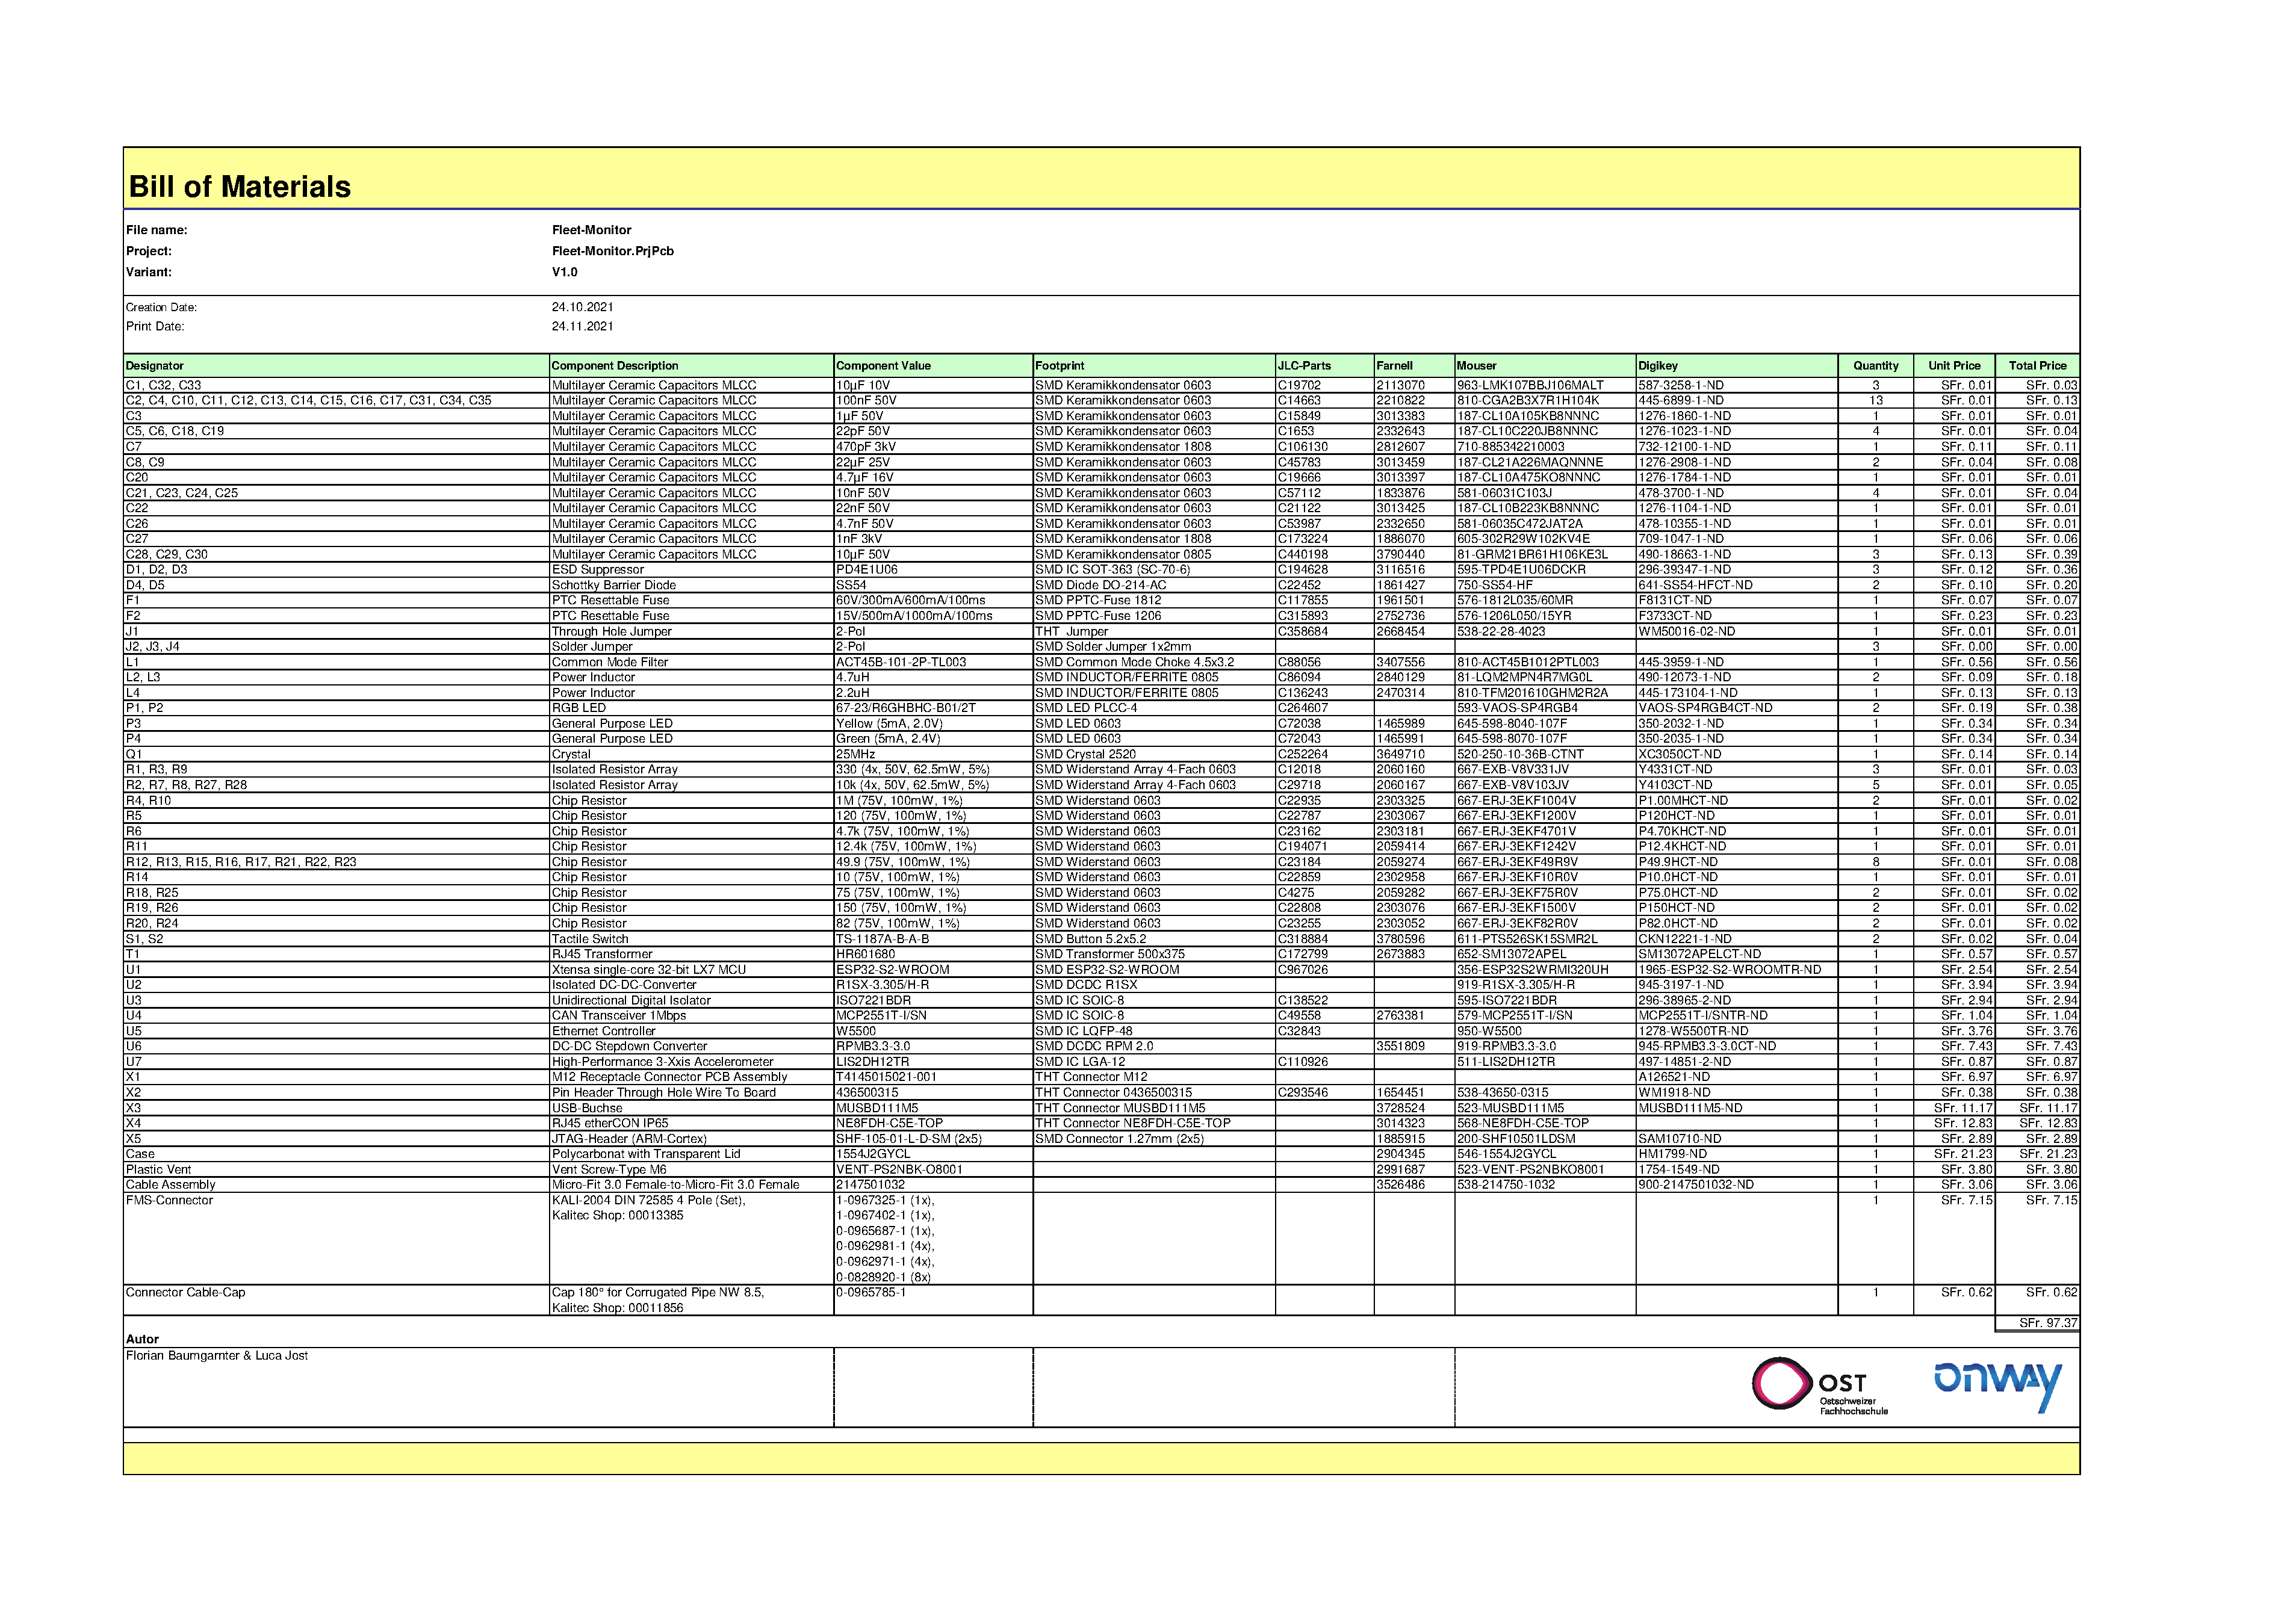
\includegraphics[angle=90, width=16.5cm]{appendix/Fleet-Monitor_BOM_croped}}
\end{adjustwidth}
\newpage


\section{Fleet-Monitor V1.0 PCB Layout} \label{Fleet-Monitor V1.0 PCB Layout}
\enlargethispage{2.5cm}
\begin{adjustwidth}{0.23cm}{0cm} \hfuzz=7.0pt \vfuzz=20.0pt
\makebox[\textwidth]{\includegraphics[angle=90, width=17.3cm, page=1]{appendix/Fleet-Monitor Layout}}
\end{adjustwidth}
\newpage

\begin{adjustwidth}{-0.23cm}{0cm} \hfuzz=7.0pt \vfuzz=20.0pt
\makebox[\textwidth]{\includegraphics[angle=90, width=17.3cm, page=2]{appendix/Fleet-Monitor Layout}}
\end{adjustwidth}
\newpage

\begin{adjustwidth}{0.23cm}{0cm} \hfuzz=7.0pt \vfuzz=20.0pt
\makebox[\textwidth]{\includegraphics[angle=90, width=17.3cm, page=3]{appendix/Fleet-Monitor Layout}}
\end{adjustwidth}
\newpage

\begin{adjustwidth}{-0.23cm}{0cm} \hfuzz=7.0pt \vfuzz=20.0pt
\makebox[\textwidth]{\includegraphics[angle=90, width=17.3cm, page=4]{appendix/Fleet-Monitor Layout}}
\end{adjustwidth}
\newpage

\begin{adjustwidth}{0.23cm}{0cm} \hfuzz=7.0pt \vfuzz=20.0pt
\makebox[\textwidth]{\includegraphics[angle=90, width=17.3cm, page=5]{appendix/Fleet-Monitor Layout}}
\end{adjustwidth}
\newpage

\begin{adjustwidth}{-0.23cm}{0cm} \hfuzz=7.0pt \vfuzz=20.0pt
\makebox[\textwidth]{\includegraphics[angle=90, width=17.3cm, page=6]{appendix/Fleet-Monitor Layout}}
\end{adjustwidth}
\newpage


\section{Fleet-Monitor V1.0 Mechanical Drawing} \label{Fleet-Monitor V1.0 Mechanical Drawing}
\enlargethispage{2.5cm}
\begin{adjustwidth}{0.23cm}{0cm} \hfuzz=7.0pt \vfuzz=20.0pt
\makebox[\textwidth]{\includegraphics[angle=90, width=17.3cm, page=1]{appendix/Fleet-Monitor Case Drawing}}
\end{adjustwidth}
\newpage

\fi

\section{Datasheet Ultrasonic Transducer} \label{appendix_ma401a6}
\enlargethispage{2.5cm}
\begin{adjustwidth}{-0.23cm}{0cm} \hfuzz=7.0pt \vfuzz=20.0pt
\makebox[\textwidth]{\includegraphics[angle=0, width=17.3cm, page=1]{appendix/MA40A16}}
\end{adjustwidth}
\newpage




\section{Data Archive} \label{Data Archive}
All created files and documents of this project are publicly available on GitHub. An institution called \textbf{SA-OST-2021} (\url{https://github.com/SA-OST-2021}) has been founded which contains repositories for each individual part of the project.
A quick description of the repositories including the associated web link is listed below:

\subsubsection{fleet-monitor-admin} \label{fleet-monitor-admin} \vspace{-0.2cm}
\begin{description}
  \item[Description:] This repository contains all confidential information of the project.\vspace{-0.25cm}
  \item[URL:] \url{https://github.com/SA-OST-2021/fleet-monitor-admin}\vspace{-0.25cm}
  \item[Type:] Private\vspace{-0.25cm}
\end{description}

\subsubsection{fleet-monitor-docs} \vspace{-0.2cm}
\begin{description}
  \item[Description:] This repository contains all additional documentation of the project.\vspace{-0.25cm}
  \item[URL:] \url{https://github.com/SA-OST-2021/fleet-monitor-docs}\vspace{-0.25cm}
  \item[Type:] Public\vspace{-0.25cm}
\end{description}

\subsubsection{fleet-monitor-requirements-specification} \vspace{-0.2cm}
\begin{description}
  \hfuzz=35.0pt
  \item[Description:] This repository contains the Requirements Specification.\vspace{-0.25cm}
  \item[URL:] \url{https://github.com/SA-OST-2021/fleet-monitor-requirements-specification}\vspace{-0.25cm}
  \item[Type:] Public\vspace{-0.25cm}
\end{description}

\subsubsection{fleet-monitor-report} \vspace{-0.2cm}
\begin{description}
  \hfuzz=35.0pt
  \item[Description:] This repository contains this document.\vspace{-0.25cm}
  \item[URL:] \url{https://github.com/SA-OST-2021/fleet-monitor-report}\vspace{-0.25cm}
  \item[Type:] Public\vspace{-0.25cm}
\end{description}

\subsubsection{fleet-monitor-hardware} \vspace{-0.2cm}
\begin{description}
  \item[Description:] This repository contains hardware and mechanical related documents.\vspace{-0.25cm}
  \item[URL:] \url{https://github.com/SA-OST-2021/fleet-monitor-hardware}\vspace{-0.25cm}
  \item[Type:] Public\vspace{-0.25cm}
\end{description}

\subsubsection{fleet-monitor-embedded} \vspace{-0.2cm}
\begin{description}
  \item[Description:] This repository contains firmware source code written in C++.\vspace{-0.25cm}
  \item[URL:] \url{https://github.com/SA-OST-2021/fleet-monitor-embedded}\vspace{-0.25cm}
  \item[Type:] Public\vspace{-0.25cm}
\end{description}

\subsubsection{fleet-monitor-configuration-tool} \vspace{-0.2cm}
\begin{description}
  \item[Description:] This repository contains the filter configuration tool written in Python.\vspace{-0.25cm}
  \item[URL:] \url{https://github.com/SA-OST-2021/fleet-monitor-configuration-tool}\vspace{-0.25cm}
  \item[Type:] Public\vspace{-0.25cm}
\end{description}

\subsubsection{fleet-monitor-network-tool} \vspace{-0.2cm}
\begin{description}
  \item[Description:] This repository contains the network tool (server) written in Python.\vspace{-0.25cm}
  \item[URL:] \url{https://github.com/SA-OST-2021/fleet-monitor-network-tool}\vspace{-0.25cm}
  \item[Type:] Public\vspace{-0.25cm}
\end{description}

\subsubsection{fleet-monitor-visualizer} \vspace{-0.2cm}
\begin{description}
  \item[Description:] This repository contains the graphical data visualizer written in Python.\vspace{-0.25cm}
  \item[URL:] \url{https://github.com/SA-OST-2021/fleet-monitor-visualizer}\vspace{-0.25cm}
  \item[Type:] Public\vspace{-0.25cm}
\end{description}

\subsubsection{fleet-monitor-rasp-image} \vspace{-0.2cm}
\begin{description}
  \item[Description:] This repository contains an image of the Raspberry Pi SD-Card.\vspace{-0.25cm}
  \item[URL:] \url{https://github.com/SA-OST-2021/fleet-monitor-rasp-image}\vspace{-0.25cm}
  \item[Type:] Public\vspace{-0.25cm}
\end{description}

\backmatter

\bibliographystyle{plain}
\typeout{}
\bibliography{./sections/bibliography.bib}

\end{document}